% Main dissertation document
\documentclass[12pt,a4paper]{report}

% Section numbering without chapter prefix
\renewcommand{\thesection}{\arabic{section}}

% Roman numerals
\newcommand{\RNum}[1]{\uppercase\expandafter{\romannumeral #1\relax}}

% Required packages
\usepackage{mathptmx}
\usepackage[utf8]{inputenc}
\usepackage[T1]{fontenc}
\usepackage{graphicx}
\usepackage{tabularx}
\usepackage{xltabular}
\usepackage{float}
\usepackage{amsmath}
\usepackage{amssymb}
\usepackage[style=apa,backend=biber]{biblatex}
\usepackage{hyperref}
\hypersetup{
    hidelinks,
    colorlinks=false
}
\usepackage{cleveref}
\usepackage[english]{babel}
\usepackage[autostyle, english=american]{csquotes}
\MakeOuterQuote{"}

% Bibliography file
\addbibresource{references.bib}

% Document settings
\setlength{\parindent}{1em}
\setlength{\parskip}{1em}
\setcounter{tocdepth}{1}

% Page numbering (roman)
\pagenumbering{roman}

\begin{document}

% Front matter
\begin{titlepage}
    \begin{center}
        \vspace*{2cm}

        \Large
        {\bf THREE PAPERS ON STRATIFICATION, FAMILY, AND WELL-BEING}

        \vspace{4cm}

        \large
        YANWEN WANG

        \vfill

        \normalsize
        A DISSERTATION SUBMITTED\\[0.3cm]
        FOR THE DEGREE OF DOCTOR OF PHILOSOPHY (SOCIOLOGY)\\
        DEPARTMENT OF SOCIOLOGY AND ANTHROPOLOGY\\
        NATIONAL UNIVERSITY OF SINGAPORE\\[2cm]

        2025

    \end{center}
\end{titlepage}
\begin{center}
    {\large \textbf{DECLARATION}}
\end{center}

\vspace{3cm}

\begin{center}
    I hereby declare that the dissertation is my original work and it has
    been written by me in its entirety. I have duly
    acknowledged all the sources of information which have
    been used in the dissertation.

    \vspace{1cm}

    This dissertation has also not been submitted for any degree in any
    university previously.

    \vspace{4cm}

    
\includegraphics[width=5cm]{misc./signature.png}\\[0.5cm]
    Yanwen Wang\\
    24 June 2025
\end{center}

\thispagestyle{plain}
\clearpage
\begin{center}
    {\large \textbf{ACKNOWLEDGEMENTS}}
\end{center}

\thispagestyle{plain}

I owe my deepest gratitude to my advisor and chair, Dr. Zheng Mu, who responded to my cold call in 2021 and with whom I have had the utmost pleasure of conducting research since then. She has supported me to the fullest, teaching me critical thinking, sociological reasoning, research design, and academic writing while giving me the freedom to explore my own interests. She is not only an outstanding mentor but also a cherished friend. She embodies the kind of scholar, mentor, and individual I aspire to become. Without her guidance and support, none of this would have been possible.

I'm also incredibly grateful to my committee members, Prof. Bussarawan Puk Teerawichitchainan and Dr. Senhu Wang, and my examiners, Prof. Vincent Chua and Prof. Kriti Vikram, for their unwavering support and evaluation of my work. From the Qualifying Examination to the Oral Defense, they have read the manuscripts multiple times and provided me with invaluable feedback that was integral in transforming simple curiosities and ideas into academic publications. Prof. Puk has taught me extensively about social demography and the importance of meticulous data analysis and coherent argumentation, Dr. Wang has helped me sharpen my research design and methodological rigor, and Prof. Chua and Prof. Vikram have provided me with invaluable feedback on both this work and future research.

I would also like to express my heartfelt thanks to my friends in Singapore. Without Linqiu Li and Shan Yang, both incredibly kind and courageous individuals, I would not have been able to navigate the ups and downs of my personal and academic life. I am also deeply grateful to my peers Ya Guo, Jinhan Liu, Nanxun Li, and Xinyi Chen, who have been exceptional friends and colleagues. Sasha and Charlie, two community cats, have also found a special place in my heart during and beyond my time in Singapore.

Finally, I want to express my profound gratitude to those closest: my parents, who have always been my strongest supporters and greatest inspirations, my fluffy friend Harvard, who taught me love, and my beloved partner Anni Ni, whose love and companionship have transformed my life in ways words can barely capture. Together, they have made these past four years the most beautiful chapter of my life. This dissertation is as much a testament to their love and support as it is to my academic endeavors.

\clearpage
\begin{center}
    {\large \textbf{SUMMARY}}
\end{center}

\thispagestyle{plain}

One of the foremost concerns today is the growing inequality in nearly all aspects of life. This dissertation on stratification, family, and well-being examines the changing patterns of family formation and how individuals and their family members are impacted by family-related stratification-generating mechanisms (e.g., intergenerational mobility, mate selection).

Specifically, Chapter 2 addresses the well-being outcome of intergenerational educational mobility, for Chinese families. It is the first to encompass both adult children and their parents, with attention to family structures and parent-child gender dynamics. Employing the Diagonal Mobility Model (DMM) to analyze data from the China Family Panel Studies, I found that net of origin and destination, those moving upwards were not necessarily better off, but both generations' well-being was impaired by downward mobility—a phenomenon observed exclusively among only-child families. Among these parents, mothers with an upwardly mobile daughter reported the highest life satisfaction. These findings highlight the departure from traditional son preferences and the plight of mobility—penalties for falling downwards with no returns to moving upwards—that traps both generations in only-child Chinese families.

Chapter 3 investigates the association between educational sorting-the spousal difference in education-and subjective well-being of heterosexual partners in Europe. It extends the literature by exploring how these associations differ between genders and vary across societies and normative climates. Using the DMM to analyze data from the European Social Survey, I found that net of status effects, hypergamy (women partnering with more educated men) was associated with lower well-being for both genders, and men were more satisfied with life in hypogamy (partnering with more educated women). Notably, women's well-being disadvantage in hypergamy was exacerbated in contexts where such partnerships were less normative. In other words, hypergamy may become even more unfavorable for women over time, as a further decline in hypergamy is likely in the foreseeable future.

Chapter 4 documents and explains the trends in marital sorting by education in China, using a decomposition approach to unpack the specific contributions of educational expansion, educational gradients in marriage rates, and assortative mating preferences. Results indicate that the initial decrease in homogamy among cohorts born before 1965 were driven entirely by educational expansion. For later cohorts, sustained educational expansion became unfavorable for hypergamy, outweighing the opposing effects of a steeper decline in marriage rates among highly educated women. Preferences for homogamy and against heterogamy, especially hypogamy, intensified. Together, these factors explained the rising homogamy, the declining hypergamy, the stagnant hypogamy, as well as the converging urban-rural disparities across later cohorts.

This dissertation contributes to a more nuanced understanding of the experience of families in the context of stratification. Future research should explore the emergence of non-conventional family forms and the broader implications of stratification.

\clearpage

% Table of contents and lists
\tableofcontents
\clearpage
\listoftables
\clearpage
\listoffigures
\clearpage

% Page numbering (arabic)
\pagenumbering{arabic}

% Main chapters
\chapter{Introduction}
\label{chap:introduction}

One of the foremost concerns today is the growing inequality in nearly all aspects of life. This is alarming across the globe and especially in developing countries like China, where various forms of inequality, whether by gender, education, ethnicity, health, or well-being, that were once byproducts of the bygone burgeoning economy, have now become its haunting aftermath \parencite{sicularUrbanRuralIncomeGap2007,xieIncomeInequalityTodays2014,yeungHigherEducationExpansion2013}. Boundaries across social groups are becoming increasingly difficult to cross, and gender relations have backslidden due to the resurgence of patriarchal values \parencite{jiUnequalCareUnequal2017}. Perhaps no other institution has experienced these repercussions more profoundly than families, and none other than families, through evolving patterns of union formation, reproduction, and relationship dynamics, holds greater potential as sources of social change.

Against this backdrop, this dissertation consists of three papers on stratification, family, and subjective well-being. Specifically, I embrace the perspective of linked lives and examine how individuals and their family members' well-being is impacted by three important family-related, stratification-associated, and relationship-oriented factors: intergenerational mobility, educational sorting in unions, and trust.

Chapter~\ref{chap:edu-mobility-swb} addresses how intergenerational mobility affects the well-being of Chinese families. It is the first to extend beyond primary movers and encompass their parents, with an emphasis on family structures and parent-child gender dynamics. Using the Diagonal Mobility Model (DMM) to analyze data from the China Family Panel Studies, I found that net of origin and destination, those moving upwards were not necessarily better off, but both generations' well-being was impaired by downward mobility—a phenomenon observed exclusively among only-child families. Among these parents, mothers with an upwardly mobile daughter reported the highest life satisfaction. These findings highlight the departure from traditional son preferences and the plight of mobility—penalties for falling downwards with no returns to moving upwards—that traps both generations in only-child Chinese families.

Chapter~\ref{chap:edu-sorting-swb} shifts the attention from intergenerational mobility to educational sorting in unions. It is a comparative study that investigates the association between educational sorting \textit{per se} and subjective well-being of heterosexual partners in Europe, with a focus on gender and contextual variations. Using the DMM to analyze data from the European Social Survey, I found that net of status effects, hypergamy (women partnering with more educated men) was associated with lower well-being for both genders, and men were more satisfied with life in hypogamy (partnering with more educated women). These patterns varied across societies, illustrated, for instance, by a hypergamy advantage among men in Southern Europe and women in the Baltic States. Notably, women's well-being disadvantage in hypergamy was exacerbated in contexts where such partnerships were less normative. These findings provide unique insights into the diverse well-being outcomes of educational sorting between genders and across societies, shaped, in part, by societal norms.

While the above chapters have examined status comparisons within families and by extension, stratification, Chapter~\ref{chap:trust-swb} focuses on trust as a critical determinant of couples' subjective well-being. Viewing both trust and well-being as multidimensional and relational constructs, this study explores how generalized and particularized trust, both measured using survey items sensitive to the "trust radius" in China, influences individuals' and their married spouse's subjective well-being across multiple dimensions—life satisfaction, happiness, and depression—via relational pathways. Lagged Actor-Partner Interdependence Models with Mediation were employed to analyze a sample of 6,964 pairs of married couples selected from the China Family Panel Studies in 2014 and 2018. Results show that particularized trust, through improving marital satisfaction and interpersonal relationships, significantly enhanced individuals' well-being in all dimensions and extended its benefits from husbands to wives, but not vice versa. Generalized trust had limited effects and did not spill over. These findings highlight the gendered dynamics within husband-wife dyadic interactions and underscore the importance of relational contexts in shaping the well-being implications of trust.

\chapter{Educational Mobility and Subjective Well-Being from an Intergenerational Perspective}
\label{chap:edu-mobility-swb}

% Input individual section files
\section{Introduction}
\label{sec:ch2-introduction}

% Introduction
Intergenerational educational mobility, defined as the upward or downward movement across parents' (origin) and adult children's (destination) educational statuses, has garnered much research attention. Sociological studies on this topic can be broadly categorized into three strands. The first describes the trends and magnitudes of educational mobility across contexts (e.g., \cite{gruijtersTrendsEducationalMobility2019,songLongtermDeclineIntergenerational2020,torcheEducationalMobilityDeveloping2021,xieTrendsSocialMobility2022}). Fueled by global educational expansion, there has been a notable increase in upward educational mobility. The proportions of children having higher education than their parents peaked at 65\% in the 1950s cohorts in high-income countries and 50\% in the 1960s cohorts in developing regions, but both were followed by decades of stagnation and in some cases, decline \parencite{torcheEducationalMobilityDeveloping2021}. The second strand addresses the societal implications of mobility, particularly concerning social stratification and inequality (e.g., \cite{bianChineseSocialStratification2002,goldthorpeSocialMobilityClass1980,yeungHigherEducationExpansion2013}). Generally agreed upon, societies with less rigid intergenerational transmission of status are more equal. The third strand, marking a transition from objective to subjective, from macro to micro, focuses on individuals' subjective experience of ascending or descending the social ladder, with which this study aligns (e.g., \cite{dhooreSocialMobilityLife2019,kwonImpactIntergenerationalMobility2022,schuckDoesIntergenerationalEducational2018,zangFrustratedAchieversSatisfied2016}).

The well-being consequences of educational mobility have been extensively theorized, with a focus on \textit{primary movers}—individuals who themselves move up or down the educational ladder. \textcite{blauSocialMobilityInterpersonal1956} conceptualized mobility as an acculturation process, wherein primary movers, neither fully integrated into the destination class nor completely constrained by their origin, were influenced by the normative beliefs, attitudes, and behaviors at both origin and destination. Other scholars emphasize the symbolic significance of mobility \textit{per se}, that is, the difference between origin and destination, which may independently affect individuals' well-being via the success or failure of fulfilling personal, familial, and societal expectations, or social isolation from both positions \parencite{michalosMultipleDiscrepanciesTheory1985,sorokin1927social,sorokin1959social}. However, empirical evaluation of these theories has long been hindered by the lack of methodological tools to disentangle the linear dependency among origin, destination, and mobility, until the introduction of the Diagonal Mobility Model (DMM) \parencite{sobelDiagonalMobilityModels1981}. The DMM, which will be reviewed in detail in the methods section, treats non-mobile individuals as the core of their respective social positions and allows for the isolation of net mobility from the respective influence of origin and destination. Using this approach, studies have found that primary movers' subjective well-being is influenced by both their parents' and their own statuses, with the latter of greater influence across contexts \parencite{dhooreSocialMobilityLife2019,kwonImpactIntergenerationalMobility2022,schuckDoesIntergenerationalEducational2018,zangFrustratedAchieversSatisfied2016}. A few exceptions notwithstanding \parencite{schuckDoesIntergenerationalEducational2018}, most studies did not find any additional mobility effects once statuses have been accounted for.

In recent years, the linked lives perspective has gained prominence in family research \parencite{bengtsonLifecoursePerspectiveAgeing2005,elderFamiliesLivesDevelopments1987,elderFamilyHistoryLife1977,macmillanFamiliesLifeCourse2005}. It recognizes that an individual's life is embedded in the family and intertwined with the lives of other family members. Given the strong connections between parents and children throughout the life course, the well-being ramifications of educational mobility will likely reverberate across generations, extending beyond primary movers to their parents. This is especially pertinent in the Chinese context, where education is viewed as a family asset, upward mobility is pursued as a family project, and parents harbor high aspiration for children's success, along with deep-seated fear of falling downward \parencite{chenEducationFeverChina2021,guSacrificeIndebtednessIntergenerational2022,guSacrificeIndebtednessIntergenerational2022,mengWhenAnxiousMothers2020}. While studies have shown that older parents' psychological well-being is strongly influenced by various life events and conditions of their children, including health, marriage, and education \parencite{friedmanSchoolingOffspringSurvival2014,maDoesAdultChildrens2022,zhangChildrensTransitionsAdulthood2023}, the association between children's educational mobility and parents' well-being remains unexplored.

By including parents and contextualizing educational mobility in intergenerational relationships, the study further draws attention to family structures and their roles in shaping both generations' subjective experience of mobility. Particularly noteworthy is the rise of only-child families as a result of the historical One-Child Policy implemented between 1979 and 2015 \parencite{settlesOneChildPolicyIts2013}. In such families, the only child, regardless of gender, enjoys exclusive access to educational resources and represents the family's sole opportunity for upward intergenerational mobility \parencite{falboQuantitativeReviewOnly1986}. This unique context allows me to address two underexplored research gaps. First, regarding the primary movers, it remains uncertain whether educational mobility is of greater consequence, in either positive or negative way, to the well-being of only children compared to those with siblings. Second, the growing prevalent of only-child families has improved gender equality, yet it remains too optimistic to conclude a thorough elimination of traditional son preferences by only-child status without an empirical comparison between only-son and only-daughter families \parencite{fongChinasOneChildPolicy2002,liuBoysOnlychildrenGirls2006,wuFertilityDeclineWomens2014}. Furthermore, the extent to which son preferences are endorsed—in this case, undermined by the only-child status—may vary between fathers and mothers \parencite{sunAreMothersSons2017}, and the intergenerational transmission of status and gender ideology are distinct by parent-child pairwise dyad \parencite{huGenderEducationExpansion2023}. These nuanced gender dynamics within only-child families have largely remained unexplored with regard to the well-being outcomes of mobility. This study addresses these issues by analyzing whether only children's subjective experiences of educational mobility vary by gender and differ from those with siblings, and whether those of fathers and mothers differ based on the child's gender.

This study focuses on the Chinese context where educational mobility is widely regarded as the primary route to broader social mobility, and only-child families have become predominant due to the historical One-Child Policy \parencite{settlesOneChildPolicyIts2013}. I utilize the DMM to analyze a representative sample of 1475 adult children and 3808 parents from only-child families, as well as 16,385 primary movers unrestricted by the only-child status, selected from the China Family Panel Studies (CFPS) in 2010. I assess the extent to which educational mobility, as well as educational statuses at origin and destination, affects the subjective well-being of both primary movers and their parents. Additionally, I examine if such influence varies by gender and only-child status.

The article is organized as follows. I begin by reviewing the theoretical framework and raising hypotheses, followed by detailing the data, measures, and analytical strategies. I then present descriptive statistics and empirical findings and conclude by summarizing the results and discussing their limitations and implications for future mobility research.

\section{Theoretical Framework}
\label{sec:ch2-theoretical-framework}

\subsection{Educational Mobility and Subjective Well-Being}

Theories on the subjective well-being outcomes of mobility, albeit diverse in perspectives and propositions, converge on two key aspects: their focus on primary movers and the conceptualization of intergenerational mobility in terms to three essential components—parents' status (origin), individuals' own status (destination), and net mobility. Each component may have independent effects, and jointly, they deem mobility consequential to primary movers' subjective well-being.

\citeauthor{blauSocialMobilityInterpersonal1956}'s (\citeyear{blauSocialMobilityInterpersonal1956})
acculturation theory emphasizes the impact of origin and destination statuses on primary movers' subjective well-being. As individuals ascend or descend the social ladder, they may find themselves neither fully acculturated to the value and lifestyles of the destination class nor entirely constrained by the origin. At an intermediate position, their normative beliefs, behaviors, and well-being are under the concurrent influence of origin and destination. In the context of educational mobility, \citeauthor{blauSocialMobilityInterpersonal1956}'s theory suggests that the educational statuses of both individuals and their parents are likely strong predictors of well-being. However, while the relative influence of the two statuses—the degree of influence by one compared to the other—may reflect the intermediate positions of primary movers, it does not account for the influence of mobility \textit{per se}, that is, the difference between origin and destination.

Other theories, while acknowledging the influence of educational statuses, underscore the independent effects of mobility. The Multiple Discrepancies Theory (MDT) posits that individuals' subjective wellbeing is largely determined by the perceived discrepancies between expectations and realities in various life domains, including education \parencite{michalosMultipleDiscrepanciesTheory1985}. Accordingly, upward mobility, which aligns with personal, familial, and societal expectations, tends to enhance life satisfaction. In contrast, those experiencing downward mobility or stagnation may feel relatively deprived. \citeauthor{newmanFallingGraceDownward1999}'s (\citeyear{newmanFallingGraceDownward1999}) anthropological work delved into the lives of individuals in downward mobility in the United States and noted that the age of affluence had exacerbated their tormented experience of "falling from grace." When upward mobility has become an assumed given, as is the case in China during mass educational expansion \parencite{xieTrendsSocialMobility2022,yeungHigherEducationExpansion2013}, the detrimental effects of falling downward are likely amplified, becoming more substantial than the benefits of upward mobility.

Still, mobility in either direction can be disruptive. \citeauthor{sorokin1927social}'s (\citeyear{sorokin1927social}) dissociative theory points to the psychological toll experienced by individuals transitioning between positions, often feeling estranged from both. It was concurred by \citeauthor{straussContextsSocialMobility1971}'s (\citeyear{straussContextsSocialMobility1971}) qualitative interviews with upwardly mobile individuals, who expressed a sense of discontinuity with their enduring identities and disappointment on arrival in search for a yet higher position. In opposition, \textcite{goldthorpeSocialMobilityClass1980} found little support for the dissociative theory, probably because upwardly mobile individuals in large numbers formed their own groups, established extensive social contacts, and thereby avoided marginalization.

These theories concertedly suggest that the three components of intergenerational educational mobility—individuals' education, parents' education, and net mobility—are all potential sources of influence. Distinguishing them apart is meaningful and crucial for understanding faithfully the well-being consequences of educational mobility. While early quantitative studies lacked the tools to disentangle their linear dependency, recent studies using the DMM have yielded mixed evidence across contexts. For example, \textcite{schuckDoesIntergenerationalEducational2018} found that in most parts of Europe, individuals' subjective well-being was influenced simultaneously by their own and their parents' education, with the former exerting a greater relative influence. Only in Continental Europe, where education was most salient for reproducing social stratification, were independent mobility effects observed: positive for those moving upward and negative for those on downward trajectories. In China, mobility studies, though not specifically on educational mobility, estimated that the relative influence of individuals' and parents' status on primary movers' well-being was approximately 3 to 1, and did not find any independent mobility effects once statuses have been accounted for \parencite{zangFrustratedAchieversSatisfied2016,zhaoDifferentialAcculturationStudy2019,zhaoInterIntragenerationalSocial2017}.

To date, theories and empirical studies have centered on primary movers and fallen short of contextualizing the experience of mobility in intergenerational relationships. This oversight is largely due to the insufficient recognition of intergenerational mobility as a family project, in which family members, especially parents, are extensively involved. In the next section, I embrace the linked lives perspective and discuss the first contribution of this study, that is, the extension of the theoretical frameworks to encompass the older generation.

\subsection{Parents at the Other End of Educational Mobility}

The idea of linked lives—"the embeddedness of human lives in social relationships of kin and friends that extend across the life span"—is key to understanding the intergenerational mutual influence between parents and children throughout the life course \parencite{elderFamiliesLivesDevelopments1987,macmillanFamiliesLifeCourse2005}. While a growing body of literature, from the perspective of linked lives, has demonstrated that parents' well-being is strongly influenced by life events and conditions of children, including health, marriage, education, and employment (e.g., \cite{friedmanSchoolingOffspringSurvival2014,maDoesAdultChildrens2022,zhangChildrensTransitionsAdulthood2023}), research on the c sequences of mobility is largely limited to primary movers. This study argues that educational mobility is a family project in which both parents and children are highly involved, thus the well-being implications of educational mobility likely resonate across generations. Specifically, I posit that the extant theoretical framework—mobility as a concurrent influence of origin, destination, and net mobility—is suitable for explaining parents' subjective experience of children's educational mobility.

First, parents' subjective well-being is strongly associated with not only their own education but also their children's \parencite{chenEducationFeverChina2021,maDoesAdultChildrens2022}. Studies on intergenerational reciprocity have shown that parents of more educated children receive from them more resources and fewer demands, which leads to lower mortality risks and better mental health \parencite{friedmanSchoolingOffspringSurvival2014,maDoesAdultChildrens2022}. In China, without the need to trace down the cause, parents' extensive, sometimes frenetic involvement in children's education is itself the best illustration of how much children's education means for parents' well-being. They participate extensively in their children's homework and school activities, spend large sums on extracurricular courses, and even purchase expensive apartments near elite schools for admission \parencite{fengSchoolQualityHousing2013,zhouFamilySocioeconomicEffect2015}. \textcite{chenEducationFeverChina2021} found that even for school-aged children, long before any material returns, their class rankings had already significantly affected parents' life satisfaction, particularly among urban, middle-class, and only-child families. \textcite{tongChildrensAcademicPerformance2021} found that parents' subjective well-being was strongly associated with both the learning efforts and academic performance of their children.

Second, mobility should be distinguished apart, with a potentially standalone effect on parents' subjective well-being. In China, parents harbor high aspirations not only for their children's educational achievement but also for upward mobility \parencite{duChinesePerceiveUpward2021}. \textcite{guSacrificeIndebtednessIntergenerational2022} pointed out that children's education, pursued as a family project, was deeply rooted in families' social mobility aspirations. \textcite{xuHopingPhoenixShanghai2013} interviewed Shanghai fathers with daughters and reported that the fathers, regardless of their own education level and despite involving less than mothers, strongly expected their daughters to exceed themselves, and regarded the fulfillment of such aspirations as their most important responsibilities.

Accompanying the highly esteemed upward mobility are the desire for status maintenance and the avoidance of downward mobility, both of which are key motives behind families' educational decisions \parencite{breenExplainingEducationalDifferentials1997,mengWhenAnxiousMothers2020}. This is especially relevant in the Chinese context where the pace of educational expansion has slowed down, the once taken-for-granted upward mobility has been hindered \parencite{yeungHigherEducationExpansion2013}. Several scholars have noted the pervasive and deep-seated fear of falling downward, which compels parents to secure their social status by every possible means, including strengthening their children's educational capital \parencite{ehrenreichFearFallingInner1989,mengWhenAnxiousMothers2020}. Thus, downward mobility is often considered the worst scenario, with its detrimental impact outweighing the potential benefits of upward mobility.

In extending mobility theories to include parents, I am sensitive toward the potential differences between fathers' and mothers' subjective experience of children's educational mobility. Though both parents aspire for their children's educational achievement and upward mobility, mothers often engage more intensively in children's educational activities, adhering to child-centered, time-consuming, self-sacrificing “intensive mothering” practices \parencite{mengWhenAnxiousMothers2020,muChangingPatternsDeterminants2022}. Considering these gender differences in parenting intensity, I expect children's education and mobility to have a more pronounced impact on mothers' subjective well-being compared to fathers.

\subsection{Gender Dynamics and Only-Child Families}

The second contribution of this study, in extending the theoretical framework to include parents, is the investigation into the roles of family structures in shaping the well-being outcomes of intergenerational educational mobility. Here, I focus on one of the most striking demographic shifts in China during the past few decades—the rise of only-child families. By the end of the One-Child Policy in 2015, only-child families have accounted for 65.6\% of all families with children. With sustained sub-replacement fertility rates, the percentage has continued to rise.

My first step is to compare only children with those who have siblings. Previous literature on the unique intergenerational dynamics in only-child families has laid a solid foundation for theorization \parencite{falboQuantitativeReviewOnly1986}. Being an only child often means receiving undivided parental attention and resources, leading to more responsive, intimate, and higher-quality parent-child relationships \parencite{liuWhoBenefitsBeing2021}. Only children often outperform others in academic performance and educational attainment \parencite{falboQuantitativeReviewOnly1986}. These advantages may translate to only children's unique subjective experience of educational mobility in two ways. First, the lack of resource dilution allows them to be more dependent on their parents \parencite{liuWhoBenefitsBeing2021}. Parents' education, in relation to their own, may be of greater relative influence compared to children with siblings. Second, the privileges associated with only-child status may come at a cost. Being the family's sole hope for upward mobility, only children could not afford to fail parental expectations and thus may experience heightened ramifications of mobility, particularly in the worst scenario of falling downward.

My second step, informed by the literature on gender equality and fertility decline, is to examine whether gender dynamics within only-child families affect the subjective experience of mobility. The rise of only-child families, in which the child, regardless of gender, receives full educational support from parents, has significantly eroded traditional son preferences that dominated much of China's history. Using the One-Child Policy as an exogenous factor, \textcite{wuFertilityDeclineWomens2014} demonstrated that women's empowerment, rather than being the cause of fertility decline, was a result of the increasing prevalence of only-child families. Daughters have benefited more than sons in terms of years of schooling and subsequent occupational attainment. These phenomena have led some scholars to argue that the once heavily gendered son- and daughter-parent contracts have converged at the very least, if not in favor of daughters \parencite{fongChinasOneChildPolicy2002,guSacrificeIndebtednessIntergenerational2022,xuHopingPhoenixShanghai2013}.

However, the only-child status may not have thoroughly undermined gender stereotypic expectations. \textcite{liuBoysOnlychildrenGirls2006} interviewed a sample of parents from only-child families and reported their persistent reinforcement of gender stereotypes in educational expectation. Therefore, she suggested that without an empirical comparison between only-son and only-daughter families, it would be overly optimistic to draw from women's overall improved educational attainment the complete eradication of son preferences by the only-child status.

In addition to the comparison by the only child's gender, I further consider gender dynamics by parent-child pairwise dyad—mother-daughter, mother-son, father-daughter, father-son dyads in only-child families. \textcite{huUnmakingOccupationalGender2024}, in their theorization of the intergenerational transmission of gender ideology, distinguished homo-lineal gender-role learning from hetero-lineal gender boundary-setting, in which the same-sex parent passes on his or her gender-role attitudes to their children, and the opposite-sex parent erects gender boundaries. Their theories, in the Chinese context, apply only to daughters but not to sons, reflecting the variations not only by fathers' and mothers' distinct influence but also by the gender of the child. Furthermore, a number of studies have noted the asymmetric endorsement of traditional son preferences between fathers and mothers, as the presence of sons may lead parents to endorse more conservative gender values, yet with more pronounced influence on mothers than fathers \parencite{sunAreMothersSons2017}. Thus, though without conclusive evidence, I infer from previous studies that traditional son preferences, if having persisted within only-child families, may be endorsed by mothers to a greater extent than by fathers.

Taking stock of the literature, the current study highlights the need for investigating parental gender preferences within the context of only-child families, with consideration of potential differences between father and mothers. Specifically, I look into the gender dynamics embedded in the well-being implications of intergenerational educational mobility within only-child families. Had the traditional son preferences prevailed would only sons assume greater responsibility for achieving higher educational attainment. This translates to, first, gender differences in only children's well-being outcomes of mobility, and second, variations in parents' well-being outcomes based on the child's gender, with potential differences between fathers and mothers. I examine these gender-related differences with regard to the relative influence of the child's education (compared to parental education), as well as the effects of net mobility.

\section{Hypotheses}
\label{sec:ch2-hypotheses}

From the preceding theoretical frameworks, I formulate four sets of hypotheses concerning both primary movers and their parents.

First, the acculturation theory emphasizes the relative influence of educational statuses at the origin and destination. For analytical purposes, I purpose the acculturation hypothesis in its most strict form.

\begin{quote}
    \textbf{H1.} Subjective well-being is affected and only affected by origin and destination. Once these are accounted for, no additional mobility effects remain.
\end{quote}

Second, mobility may exert an independent effect on subjective wellbeing. The MDT suggests varying effects of mobility by direction, with downward mobility being particularly harmful \parencite{michalosMultipleDiscrepanciesTheory1985}. On the other hand, \citeauthor{sorokin1927social}'s (\citeyear{sorokin1927social}) dissociative theory posits disruptive effects of mobility in both directions. This leads to the mobility hypothesis.

\begin{quote}
    \textbf{H2.} Subjective well-being is affected by mobility, net of origin and destination.
\end{quote}

\begin{quote}
    \textbf{H2a.} Subjective well-being is positively associated with upward mobility and negatively related to downward mobility, with the latter having a larger absolute effect.
\end{quote}

\begin{quote}
    \textbf{H2b.} Subjective well-being is negatively associated with mobility in either direction.
\end{quote}

The third set of hypotheses focuses on the role of family structures in shaping the well-being outcomes of educational mobility. The only-child hypothesis compares only children with those with siblings. Drawing on traditional son preferences, the gender disparity hypotheses contrast only sons with only daughters, and parents of only son with those of only daughter, with differences between fathers and mothers.

\begin{quote}
    \textbf{H3a.} Among primary movers, the relative influence of origin on subjective well-being, as well as the effects of net mobility, is greater for only children than for those with siblings.
\end{quote}

\begin{quote}
    \textbf{H3b.} Among only children, the relative influence of destination on subjective well-being, as well as the effects of net mobility, is greater for sons than for daughters.
\end{quote}

\begin{quote}
    \textbf{H3c.} Among parents, the relative influence of destination (compared to origin), as well as the effects of net mobility, is greater for parents with an only son than for those with an only daughter. Differences by child's gender may be greater for mothers than for fathers.
\end{quote}

Lastly, acknowledging mothers' more intensive involvement in childcare, I propose:

\begin{quote}
    \textbf{H4.} Among parents, the relative influence of destination (compared to origin) on subjective well-being, as well as the effects of mobility, is greater for mothers than for fathers.
\end{quote}

\section{Data and Methods}
\label{sec:ch2-data-methods}

\subsection{Data and Sample}

The study selected samples from the China Family Panel Studies (CFPS) in 2010. The CFPS, initiated in 2010, is a biennial survey employing an implicitly stratified, multistage probability strategy to draw samples representative of China's national population \parencite{xieSamplingDesignChina2015}. It contains rich data on sociodemographic characteristics of household members, as well as subjective well-being of focal respondents, making it ideal for the present study on mobility outcomes from an intergenerational perspective. For this analysis, I chose the 2010 baseline wave because it included information on the number of siblings, enabling a straightforward identification of only-child status while minimizing sample loss.

Table~\ref{app:tab:sample_restriction_ch2} shows steps of sample restrictions. For the older generation, I first narrowed down the initial sample of 33,598 respondents to those with only one child, reducing the sample size to 10,261 by 69.46\%. I then selected parents whose child had graduated from school and aged between 20 and 50, further reducing the sample to 3836 by 62.62\%. Finally, I excluded those with missing values, dropping an additional 0.73\%. The final analytic sample of the older generation comprises 3808 parents.

For primary movers, I first restricted the sample to those who were not in school and aged between 20 and 50, reducing the sample size from 33,598 to 18,172 by 45.91\%. I then dropped those with missing values, resulting in a further 9.83\% decrease in sample size. The final analytic sample comprises 16,385 primary movers, of which 1475 were identified as only children. For intergenerational comparisons within only-child families, I present descriptive statistics for only children separately from those for all primary movers in later sections.

\subsection{Measures}

\textbf{Subjective Well-Being.} The dependent variable, subjective well-being, was measured by life satisfaction on a 1 (\textit{very dissatisfied}) to 5 (\textit{very satisfied}) scale: “overall, are you satisfied with life?” It is the most extensively used single-item question for measuring life satisfaction and a reliable indicator of subjective well-being.

\textbf{Educational Mobility.} The measure of intergenerational educational mobility is based on the comparison between parents' and children's absolute educational levels. In the Chinese context, absolute educational credential carries substantial weight in determining individuals' opportunities in the labor market and, as illustrated by \textcite{xuHopingPhoenixShanghai2013}, reflects parents' most intuitive aspiration for upward mobility, regardless of their children's relative standing among peers. Thus, I first categorized respondents' education into four levels: \textit{primary or lower}, \textit{middle school}, \textit{high school}, and \textit{college or higher}. The four-tier classification ensures adequate sample sizes at each level for both generations.

I then measured mobility by comparing the child's education with that of their highest-educated parent, an approach similar to \textcite{schuckDoesIntergenerationalEducational2018} but different from most previous studies that measured the origin by father's status only (e.g., \cite{dhooreSocialMobilityLife2019,kwonImpactIntergenerationalMobility2022,zangFrustratedAchieversSatisfied2016}). I chose this approach for two reasons. First, comparing children's status to the best that their parents have achieved is appropriate to capture the nature of educational mobility as a family project \parencite{guSacrificeIndebtednessIntergenerational2022}. Second, the mother-child status associations have been strengthened as a result of the rising hypogamy \parencite{huGenderEducationExpansion2023}. As in the sample of only children, mothers had higher education than fathers in 16.22\% of relationships in which both parents' education was identified. Thus, identifying parents' education solely by fathers' status may lead to biased measures of intergenerational educational mobility.

Thus, intergenerational educational mobility was identified as \textit{non-mobile} if the child's education matched that of their highest-educated parent, \textit{upward} if higher, and \textit{downward} if lower.

\textbf{Covariates.} I controlled several variables relevant to subjective well-being, including gender (1=\textit{female}, 0 = \textit{male}), age in continuous years, ethnicity (1 = \textit{Han Chinese}, 0 = \textit{non-Han minorities}), marital status (1 = \textit{married}, 0 = \textit{not married}), Communist Party membership (1 = \textit{party member}, 0 = \textit{non-member}), urban status (1 = \textit{urban}, 0 = \textit{rural}), and economic relationship with parents or children (1 = \textit{economically related}, 0 = \textit{not related}). In analyses of all primary movers, I also included only-child status (1 = \textit{only child}, 0 = \textit{non-only child}). Provided that the primary interest is in the overall effects of educational mobility, I did not control variables of potential mediating effects, such as income and employment status.

\subsection{Analytic Strategy}

Since the three components of intergenerational educational mobility—origin, destination, and mobility—are linearly dependent, and any two provide the remaining one, it is statistically challenging to estimate all three simultaneously by conventional linear regressions \parencite{sobelDiagonalMobilityModels1981}. One compromising strategy is to estimate the effects of mobility while controlling for either origin or destination. However, this strategy results in confounded estimations, as well summarized by \textcite{schuckDoesIntergenerationalEducational2018}. For instance, omitting the higher destination status in the case of upward mobility may lead to an overestimation of its positive influence and the neglect of its potential distress \parencite{nikolaevIntergenerationalMobilitySubjective2014}.

The Diagonal Mobility Model (DMM), also known as the Diagonal Reference Model, is a type of nonlinear models capable of modeling origin, destination, and mobility simultaneously and has become the gold standard for mobility research \parencite{sobelDiagonalMobilityModels1981,sobelSocialMobilityFertility1985,zangMobilityEffectsHypothesis2023}. The DMM is informed by the sociological assumption that non-mobile individuals build up the core of their respective social position and, for my research questions, their subjective well-being best represent the characteristics of their respective educational level. Taking this as the starting point, the DMM treats non-mobile individuals as the reference groups and models individuals' life satisfaction as a weighted sum of that of non-mobile individuals at origin and destination. The weights, which sum up to one, denote the relative influence of origin and destination on mobile individuals' subjective well-being, over and above which net mobility effects can be isolated and estimated. The baseline DMM without mobility indicators can be specified as follows:

\begin{equation}
    \label{eq:dmm-chapter2}
    \text{Y}_{ijk} = p \mu_{ii} + (1-p) \mu_{jj} + \sum \beta X_{kl} + \epsilon_{ijk}, 0 \leq p \leq 1
\end{equation}

Here, $Y_{ijk}$ is the life satisfaction of individual $k$ who moved from educational category $i$ to $j$, $\mu_{ii}$ and $\mu_{jj}$ are the life satisfaction of non-mobile individuals in categories $i$ and $j$, respectively, and $\sum \beta X_{kl}$ is a vector of covariates. Weight parameters $p$ and $(1-p)$ capture the relative influence of origin and destination.

Mobility effects can be assessed by adding mobility indicators into the baseline model, which is given by:

\begin{equation}
    \label{eq:dmm_mobility}
    \text{Y}_{ijk} = p \mu_{ii} + (1-p) \mu_{jj} + \gamma_{1} U_{k} + \gamma_{2} D_{k} + \sum \beta X_{kl} + \epsilon_{ijk}, 0 \leq p \leq 1
\end{equation}

Where $U_{k}$ and $D_{k}$ are dummy variables for upward and downward mobility of individual $k$, respectively, $\gamma_{1}$ and $\gamma_{2}$ capture net mobility effects on life satisfaction.

To evaluate the only-child hypothesis, the gender disparity hypothesis, and differences between fathers and mothers, I added interactions terms with the weights of statuses and mobility indicators separately in subsequent models. For example, the models testing the only-child hypothesis are given by:

\begin{equation}
    \label{eq:dmm_only_child}
    \text{Y}_{ijk} = (p + p_{o} O_{k}) \mu_{ii} + (1 - p - p_{o} O_{k}) \mu_{jj} + \gamma_{1} U_{k} + \sum \beta X_{kl} +\epsilon_{ijk}, 0 \leq p \leq 1
\end{equation}

\begin{equation}
    \label{eq:dmm_only_child_mobility}
    \text{Y}_{ijk} = p \mu_{ii} + (1-p) \mu_{jj} + \gamma_{uo} U_{k} O_{k} + \gamma_{do} D_{k} O_{k} + \sum \beta X_{kl} + \epsilon_{ijk}, 0 \leq p \leq 1
\end{equation}

Where $O_{k}$ stands for whether individual $k$ is an only child. The relative influence of origin increases by $p_{o}$ if individual $k$ is an only child, and that of destination decreases by the same amount. Differences in the effects of upward and downward mobility are captured by coefficients $\gamma_{uo}$ and $\gamma_{do}$ in \ref{eq:dmm_only_child_mobility}. Gender differences among only-children and their parents were assessed in similar ways.

The study used the Akaike Information Criterion (AIC) and likelihood ratio tests (LRT) to determine if additional variables lead to significant improvement in fit measures \parencite{sobelSocialMobilityFertility1985}. Models were estimated using the "gnm" package in R \parencite{turnerGnmGeneralizedNonlinear2005}.

\section{Results}
\label{sec:ch2-results}

\subsection{Descriptive Statistics}

Table~\ref{tab:descriptive_stats} summarizes the descriptive statistics for the samples. Gender-specific statistics for those from only-child families are detailed in Table~\ref{app:tab:descriptive_by_gender}. Among parents from only-child families (N = 3808), gender composition was nearly even, with 47.98\% being fathers. Sons (59.46\%) were overrepresented among only children (N = 1475), compared to 47.21\% among those with siblings. The gender imbalance among only children can be attributed to two factors. First, the historical One-Child Policy has intensified sex selection at birth in favor of sons \parencite{zhuChinasExcessMales2009}. Second, only sons are more likely than only daughters to co-reside with their parents and to be included in household-level surveys \parencite{fengChengshiDushengZinu2009}.

Parents from only-child families reported higher life satisfaction ($M$=3.43, \\$SD$=1.05) than adult children with or without siblings. They were on average 54.10 years old ($SD$=7.88), with fathers older than mothers. Over 90\% were married, and 95.69\% identified themselves as Han Chinese. Approximately one in ten were members of the Communist Party, and around two thirds (67.88\%) lived in urban areas. Most of these parents (73.82\%) considered themselves economically related to their only child.

    Among the younger generation, children with or without siblings reported similar life satisfaction. Daughters were more satisfied with life than sons. The average age of only children was 30.44 years ($SD$=7.82), significantly younger than those with siblings. Correspondingly, a smaller proportion of only children were married (64.27\%), compared to those not restricted by only-child status (85.88\%). Over 90\% were Han Chinese. Only 5.59\% were Communist Party members. Urban residency and economic relationships with parents were more common among only children than those with siblings.

Unsurprisingly, the younger generation had much higher educational attainments than their parents. Among only children, 32.54\% held college or higher degrees, 21.90\% had high school diplomas, 27.12\% had completed middle school, and only 18.44\% had primary school or lower education. In contrast, in the other two groups, 75.02\% of parents from only-child families and 74.91\% of primary movers unrestricted by only-child status did not progress beyond middle school. I found evidence consistent with the reversal of gender gaps in education, particularly among only-child families \parencite{yeungHigherEducationExpansion2013}. As shown in Table~\ref{app:tab:descriptive_by_gender}, while fathers were typically more educated than mothers, daughters have now surpassed sons in educational attainment.

Table~\ref{tab:mobility_patterns} outlines the patterns of intergenerational educational mobility among those from only-child families and all primary movers with or without siblings. Upward mobility was notably prevalent, especially among only-child families. Approximately 56\% of only children moved upward, compared to 41.67\% of those with siblings. A small but non-negligible percentage (around 10\%) of individuals in both groups experienced downward mobility. Additionally, a considerable proportion of individuals remained non-mobile at each educational level, totaling 34.14\% in only-child families and 46.87\% among those with siblings. Those non-mobile individuals are essential in the DMMs for representing their respective positions and serving as reference groups \parencite{sobelSocialMobilityFertility1985}.

\subsection{Findings}

In the first step, I replicated previous research on the subjective experience of educational mobility among primary movers. Table~\ref{tab:dmm_results} presents the results of the DMMs on life satisfaction of primary movers with or without siblings, organized in four parts: the relative influence of parents' (origin) and individuals' (destination) education, mobility indicators, diagonal intercepts of non-mobile individuals, and covariates.

The baseline model estimates the relative influence of origin and destination. Results show that the subjective well-being of primary movers was affected by both their parents' (0.29) and their own (0.71) education, with the latter of greater influence. In Model 2, I added dummy variables for upward and downward mobility. Neither was significant. This suggests that net of educational statuses at the origin and destination, mobility in either direction did not independently affect primary movers' subjective well-being. These results support the acculturation hypothesis (H1) and rejected the mobility hypotheses (H2, H2a, and H2b), with regard to primary movers. These findings are consistent with findings of other studies in China, in which individuals' own status accounted for a substantial proportion (ranging from 76\% to 79\%) of the total status effects at origin and destination, and no mobility effects were observed after accounting for statuses \parencite{zangFrustratedAchieversSatisfied2016,zhaoDifferentialAcculturationStudy2019,zhaoInterIntragenerationalSocial2017}.

In Models 3 and 4, I interacted only-child status with educational statuses and mobility indicators, respectively. Two main findings were derived from the model results. First, as shown by the non-significant interaction terms in Model 3, the relative influence of origin and destination to subjective well-being did not differ significantly between only children and those with siblings. Second, as shown in Model 4, only children on downward trajectories were less satisfied with life (-0.18) than their counterparts with siblings. These findings partially validated the only-child hypothesis (H3a).

The diagonal intercepts, detailed in Part III of Table~\ref{tab:dmm_results}, show no distinct gradient in life satisfaction among non-mobile individuals across different educational levels, suggesting that in case of stagnation, subjective well-being was not linearly associated with education. Regarding the covariates, primary movers who were female, younger, Han-Chinese, married, or members of the Communist Party reported significantly higher life satisfaction, whereas those residing in urban areas or having economic relationships with parents were less satisfied with life.

In the second stage of the analysis, I stratified the samples by only-child status. The results of the DMMs on life satisfaction of only children are summarized in Table~\ref{tab:dmm_only_children}. The subsequent discussion focuses on only children's wellbeing outcomes of mobility.

The baseline model shows that their life satisfaction was influenced by both parents' (0.40) and their own (0.60) education. While the influence of parents' education appeared to be more pronounced for only children than for those with siblings, the difference was not statistically significant, as indicated by interactions terms in earlier models. In Model 2, the additional mobility indicators significantly improved the model fits, suggesting that mobility exerted independent effects on subjective well-being, net of statuses. However, these effects were asymmetric. Only downward mobility was significantly and negatively (-0.22) associated with life satisfaction of only children, whereas upward mobility had no significant impact. These findings, with regard to only children, validated the mobility hypotheses H2 and H2a and rejected the dissociative hypothesis (H2b).

To evaluate the gender disparity hypothesis (H3b), I interacted respondents' gender with educational statuses and mobility indicators in Models 3 and 4, respectively. None of the interaction terms was significant. Thus, I rejected hypothesis H3b and concluded that the relative influence of origin and destination on subjective well-being did not differ between sons and daughters from only-child families, nor did the negative effects of downward mobility vary by gender. Intergenerational educational mobility exerted much the same influence on sons and daughters from only-child families.

No distinct gradient in life satisfaction was observed among non-mobile only children across different educational levels. Sociodemographic factors such as being female, younger, married, or Party members were associated with higher life satisfaction. Urban residency and economic relationships with parents were related to lower life satisfaction.

In the final phase of the analysis, I expanded the framework to include parents from only-child families, examining how their life satisfaction was influenced by their children's educational mobility. These results are summarized in Table~\ref{tab:dmm_only_child_parents}.

As shown by the baseline model, parents' life satisfaction was simultaneously influenced by origin (0.78) and destination (0.22), with their own status being more influential. Model 2 incorporates additional dummies of upward and downward mobility. Results indicate that parents felt less satisfied with life (-0.14) when their child experienced downward mobility but were unaffected by upward mobility.

Subsequent models (Models 3 to 6) include interactions terms to explore variations by parents' and the child's gender. Results of these models show that the relative influence of origin and destination, as well as the detrimental effects of downward mobility, did not differ between fathers and mothers, nor did it vary by the child's gender. The educational attainment and mobility of the daughter were as impactful as those of the son for parents from only-child families, pointing to a convergence, if not a reversal, of son- and daughter-parent relationships.

In Models 7 and 8, I introduced three-way interactions to determine if these patterns hold for both fathers and mothers. Notably, in Model 8, the interaction term among upward mobility, mother, and daughter was significantly positive, suggesting gender differentials by parent-child pairwise dyad. Mothers were more satisfied with life if their daughter achieved upward mobility, whereas the son's mobility did not have such effects. Among all parents, mothers with an upwardly mobile daughter reported the highest life satisfaction. On the other hand, educational mobility of the only son and the only daughter had similar effects on their fathers’ subjective well-being. These findings challenge the notion that traditional son preferences have persisted in only-child families and are more strongly endorsed by mothers than fathers \parencite{liuBoysOnlychildrenGirls2006,sunAreMothersSons2017}. Instead, they provide preliminary evidence on a maternal preference for daughters. Hypotheses H3c and H4 were thus rejected.

Contrary to the lack of a distinct gradient in life satisfaction among non-mobile primary movers across the educational ladder, I observed an overall negative gradient in life satisfaction among parents with non-mobile only children. Specifically, the levels of life satisfaction were 2.91, 2.83, 2.71, and 3.03 for those with primary school or lower, middle school, high-school diploma, and college or higher degrees, respectively. This suggests a heightened dissatisfaction with status stagnation among higher-educated parents, except for those already at the top educational level. Among the covariates, being female, older, married, party members, and living in rural areas were positively associated with life satisfaction.

From the above findings, I draw three important conclusions. First, both parents' and adult children's educational statuses were significant determinants of subjective well-being, with a relatively greater influence from individuals' own education. Second, downward mobility adversely affected subjective well-being, a phenomenon exclusively observed in only-child families, whereas upward mobility had no significant impact. Third, the son- and daughter-parent contracts in only-child families have largely converged and, to some extent, shifted in favor of the daughter.

\section{Discussion}
\label{sec:ch2-discussion}

The current study utilized the DMM to explore the well-being implications of intergenerational educational mobility for primary movers and their parents, with a focus on those from only-child families. The results indicate a concurrent influence of parents' and adult children's education on their subjective well-being, with individuals' own education being more influential. Notably, I observed distinct and asymmetric effects of mobility exclusively among only-child families: both generations experienced decreased life satisfaction in the event of downward mobility, while upward mobility did not have any significant impact. Furthermore, I did not find evidence supporting gender differentiation or traditional son preferences within only-child families.

Theoretically, I embraced the linked lives perspective and extended mobility theories to include the experiences of primary movers' parents. In the Chinese context, where education mobility is pursued as a family project, and parents harbor high aspirations for their children's upward mobility, along with deep-seated anxiety of falling downward \parencite{guSacrificeIndebtednessIntergenerational2022,guWhyChineseAdolescent2021,mengWhenAnxiousMothers2020}, I have strong reasons to expect parents' subjective well-being to be closely linked to their children's educational attainment and mobility. Furthermore, I underscore the saliency of family structures and gender dynamics in shaping well-being outcomes of mobility. In the now dominating only-child families, the child, regardless of gender, is the only hope for the family to move upward. While the progress toward gender equality owes much to the rise of only-child families, few studies have made comparisons within only-child families \parencite{fongChinasOneChildPolicy2002,liuWhoBenefitsBeing2021,wuFertilityDeclineWomens2014}. In this study, I probe whether the well-being ramifications of educational mobility are amplified for only children and whether the son- and daughter-parents relationships within only-child families have converged based on the experiences of both generations.

Empirically, the results affirmed the relevance of the acculturation theory for both primary movers and their parents in only-child families. Both generations' subjective well-being was simultaneously impacted by educational statuses at origin and destination, with individuals' own status being more influential. These findings echo previous studies on the impact of mobility on primary movers' well-being both within China and globally \parencite{dhooreSocialMobilityLife2019,kwonImpactIntergenerationalMobility2022,schuckDoesIntergenerationalEducational2018,zangFrustratedAchieversSatisfied2016}, and are in line with the extant literature on the intergenerational associations between children's education and parents' well-being \parencite{chenEducationFeverChina2021,maDoesAdultChildrens2022}.

Empirical results show that in only-child families, both generations' subjective well-being was negatively affected by downward mobility without any reward from moving upward. This was, however, not observed among those with siblings, nor by previous studies on the general Chinese population, though their data and measures of intergenerational mobility were different \parencite{zangFrustratedAchieversSatisfied2016,zhaoDifferentialAcculturationStudy2019,zhaoInterIntragenerationalSocial2017}. The unique intergenerational dynamics in only-child families, where the entire family's hope for moving upward rests on the only child, intensify the negative consequences associated with not achieving this goal. With these findings, I contend that the consequences of intergenerational mobility should be contextualized in families and examined with consideration of diverse familial settings.

Two reasons may explain why parents and children from only-child families were adversely impacted by downward mobility without benefiting from upward mobility. First, from a cognitive and psychological perspective, individuals tend to be more sensitive to the pains associated with losses—downward mobility in this case, than to the pleasures derived from equivalent gains \parencite{kahnemanAnomaliesEndowmentEffect1991}. Second, due to social comparison, individuals’ subjective well-being is influenced less by absolute gains or losses and more by their relative standing compared to others. When most individuals, especially those from only-child families, have moved upward during mass educational expansion in China, the gains from upward mobility are likely to diminish, and the losses associated with downward mobility become even more devastating.

These well-being consequences of educational mobility did not differ by gender among primary movers. Sons and daughters, with or without siblings, experienced similar outcomes. For parents from only-child families, the education and mobility of the daughter mattered as much as those of the son to fathers, and even more so to mothers. Previous studies have attributed the overall improvement in women's educational attainment in part to the rise of only-child families \parencite{fongChinasOneChildPolicy2002,wuFertilityDeclineWomens2014}. This study furthers the literature by contrasting families with only sons against those with only daughters and by exploring the dynamics between different parent-child gender pairs. Indeed, traditional son preferences have been undermined by only-child status, and the once heavily gendered son- and daughter-parent relationships have converged and, to some extent, reversed in favor of the daughter \parencite{guWhyChineseAdolescent2021}.

The study is, however, not without limitations. First, despite the strengthening mother-child status association \parencite{huGenderEducationExpansion2023}, measures of intergenerational mobility did not differentiate between the genders of parents. Incorporating both parents' education separately will add another dimension to the DMM's diagonal designs, which complicates the model and may violate its central assumption—the representation of each non-diagonal level by non-mobile individuals. Second, the same methodological concern prevented me from including multiple children's education statuses, thereby limiting the findings of parents to those from only-child families. Third, I did not investigate variations in the outcomes of mobility across the educational ladder, since the DMM averages the effects across all individuals. Fourth, the cross-sectional design of the DMM constrains my ability to thoroughly address endogeneity issues arising from individuals' selection into different mobility trajectories. Therefore, I advise caution in drawing causal inferences from the findings without the support of longitudinal data. Lastly, my analysis relies on the CPFS data collected in 2010. Considering the changes within the educational system and broader society, this temporal gap may affect the generalizability of the results to the present context.

These limitations did not diminish the strength of this study. While mobility research has predominantly focused on primary movers, I demonstrated the importance of embracing the perspective of linked lives in contextualizing educational mobility within intergenerational relationships and recognizing its nature as a family project. Findings showed that educational mobility mattered not only to primary movers but also to their parents, with outcomes conditioned by the only-child family structure and parent-child gender dynamics. These insights, along with identified limitations, pave new avenue for future research, including but not limited to employing gender-sensitive mobility measures, addressing family dynamics with multiple children with attention to gender and birth order, and exploring heterogeneous mobility effects across social strata. Future research may also leverage more recent data to investigate the complex interplay between individual mobility and broader structural changes. This may involve developing contextual-level indexes to capture the degree of competitiveness for moving upward or measuring relative educational mobility by comparing the relative educational positions of parents and children within their respective temporal and spatial groups, both of which, however, have not been accomplished by the current study. Moreover, I call for future studies to incorporate other dimensions of intergenerational mobility, such as occupational and income mobility, and to assess the universality or specificity of these findings across different contexts, to better understand the full spectrum of social stratification and its implications for well-being.


% Input tables and figures

\begin{table}[H]
    \caption{Descriptive statistics of the samples.}
    \label{tab:descriptive_stats}
    \setlength{\tabcolsep}{1.2em}
    \renewcommand{\arraystretch}{1.2}
    \begin{tabularx}{\textwidth}{@{} l|*{3}{>{\centering\arraybackslash}X} @{}}
        \hline
                                       & Parents      & Only children & Primary movers \\
        \hline
        Life satisfaction              & 3.43 (1.05)  & 3.36 (1.01)   & 3.39 (1.04)    \\
        Age                            & 54.10 (7.88) & 30.44 (7.82)  & 36.72 (8.43)   \\
        Minority                       & 0.04 (0.20)  & 0.05 (0.22)   & 0.09 (0.29)    \\
        Married                        & 0.90 (0.29)  & 0.64 (0.48)   & 0.86 (0.35)    \\
        Party member                   & 0.12 (0.32)  & 0.06 (0.25)   & 0.06 (0.23)    \\
        Urban                          & 0.68 (0.47)  & 0.71 (0.46)   & 0.45 (0.50)    \\
        Economically related           & 0.74 (0.44)  & 0.62 (0.49)   & 0.30 (0.46)    \\
        \textit{Education}                                                             \\
        \hspace{0.5cm}Primary or lower & 40.99\%      & 18.44\%       & 40.09\%        \\
        \hspace{0.5cm}Middle school    & 34.03\%      & 27.12\%       & 34.82\%        \\
        \hspace{0.5cm}High school      & 18.72\%      & 21.90\%       & 14.95\%        \\
        \hspace{0.5cm}College or above & 6.22\%       & 32.54\%       & 10.14\%        \\
        Total                          & 3808         & 1475          & 16385          \\
        \hline
    \end{tabularx}
    \begin{flushleft}
        \small
        \textit{Notes:} Standard deviations are presented in parentheses.
    \end{flushleft}
\end{table}

\begin{table}[H]
    \caption{Patterns of educational mobility.}
    \label{tab:mobility_patterns}
    \setlength{\tabcolsep}{1.2em}
    \renewcommand{\arraystretch}{1.2}
    \begin{tabularx}{\textwidth}{@{} l|*{4}{>{\centering\arraybackslash}X} @{}}
        \hline
        \multicolumn{5}{l}{Sample: Parents (N = 3808)}          \\
        \hline
        Child/Parents & Level 1 & Level 2 & Level 3 & Level 4   \\
        \hline
        Level 1       & 30.19\% & 5.46\%  & 2.53\%  & 1.30\%    \\
        Level 2       & 41.52\% & 30.73\% & 13.89\% & 5.21\%    \\
        Level 3       & 15.40\% & 27.85\% & 28.84\% & 20.05\%   \\
        Level 4       & 12.89\% & 35.96\% & 54.74\% & 73.44\%   \\
        \hline
        \multicolumn{5}{l}{Sample: Only children (N = 1475)}    \\
        \hline
        Child/Parents & Level 1 & Level 2 & Level 3 & Level 4   \\
        \hline
        Level 1       & 39.23\% & 9.38\%  & 4.19\%  & 0.00\%    \\
        Level 2       & 38.67\% & 26.67\% & 16.17\% & 6.78\%    \\
        Level 3       & 14.00\% & 30.83\% & 22.75\% & 19.49\%   \\
        Level 4       & 8.10\%  & 33.12\% & 56.89\% & 73.73\%   \\
        \hline
        \multicolumn{5}{l}{Sample: Primary movers (N = 16,385)} \\
        \hline
        Child/Parents & Level 1 & Level 2 & Level 3 & Level 4   \\
        \hline
        Level 1       & 50.60\% & 22.99\% & 16.76\% & 5.90\%    \\
        Level 2       & 34.05\% & 41.23\% & 32.25\% & 16.10\%   \\
        Level 3       & 11.16\% & 21.69\% & 22.95\% & 24.72\%   \\
        Level 4       & 4.18\%  & 14.10\% & 28.04\% & 53.29\%   \\
        \hline
    \end{tabularx}
\end{table}

\begin{xltabular}{\textwidth}{@{} l|*{4}{>{\centering\arraybackslash}X} @{}}
    \caption{DMM on life satisfaction of primary movers.}
    \label{tab:dmm_results} \\
    \hline
    & Model 1   & Model 2   & Model 3   & Model 4   \\
    \hline
    \endfirsthead
    \multicolumn{5}{l}{\tablename\ \thetable{} -- continued from previous page} \\
    \hline
    & Model 1   & Model 2   & Model 3   & Model 4   \\
    \hline
    \endhead
    \hline \multicolumn{5}{r}{\textit{Continued on next page}} \\
    \endfoot
    \hline
    \endlastfoot
    \multicolumn{5}{l}{\textit{Part \RNum{1}: Weight parameters}} \\
    Origin               & 0.29*     & 0.19      & 0.25      & 0.18      \\
    & (0.14)    & (0.18)    & (0.15)    & (0.19)    \\
    * only child         &           &           & 0.21      &           \\
    &           &           & (0.26)    &           \\
    Destination          & 0.71***   & 0.81***   & 0.75***   & 0.82***   \\
    & (0.14)    & (0.19)    & (0.15)    & (0.19)    \\
    * only child         &           &           & -0.21     &           \\
    &           &           & (0.26)    &           \\[0.3em]
    \multicolumn{5}{l}{\textit{Part \RNum{2}: Mobility indicators}} \\
    Upward               &           & -0.03     &           & -0.02     \\
    &           & (0.03)    &           & (0.03)    \\
    * only child         &           &           &           & -0.04     \\
    &           &           &           & (0.06)    \\
    Downward             &           & 0.00      &           & 0.02      \\
    &           & (0.03)    &           & (0.03)    \\
    * only child         &           &           &           & -0.18*    \\
    &           &           &           & (0.10)    \\[0.3em]
    \multicolumn{5}{l}{\textit{Part \RNum{3}: Diagonal intercepts}} \\
    Primary or lower     & 3.50***   & 3.50***   & 3.50***   & 3.49***   \\
    & (0.05)    & (0.05)    & (0.05)    & (0.05)    \\
    Middle school        & 3.58***   & 3.59***   & 3.58***   & 3.58***   \\
    & (0.05)    & (0.05)    & (0.05)    & (0.05)    \\
    High school          & 3.50***   & 3.51***   & 3.50***   & 3.51***   \\
    & (0.05)    & (0.06)    & (0.05)    & (0.06)    \\
    College or above     & 3.73***   & 3.73***   & 3.73***   & 3.72***   \\
    & (0.06)    & (0.06)    & (0.06)    & (0.06)    \\[0.3em]
    \multicolumn{5}{l}{\textit{Part \RNum{4}: Covariates}} \\
    Female               & 0.10***   & 0.10***   & 0.10***   & 0.10***   \\
    & (0.02)    & (0.02)    & (0.02)    & (0.02)    \\
    Age                  & -0.01***  & -0.01***  & -0.01***  & -0.01***  \\
    & (0.00)    & (0.00)    & (0.00)    & (0.00)    \\
    Married              & 0.33***   & 0.33***   & 0.33***   & 0.33***   \\
    & (0.03)    & (0.03)    & (0.03)    & (0.03)    \\
    Party member         & 0.21***   & 0.21***   & 0.21***   & 0.21***   \\
    & (0.04)    & (0.04)    & (0.04)    & (0.04)    \\
    Urban                & -0.11***  & -0.11***  & -0.11***  & -0.11***  \\
    & (0.02)    & (0.02)    & (0.02)    & (0.02)    \\
    Minority             & -0.08**   & -0.08**   & -0.08**   & -0.08**   \\
    & (0.03)    & (0.03)    & (0.03)    & (0.03)    \\
    Economically related & -0.04*    & -0.04     & -0.04*    & -0.04     \\
    & (0.02)    & (0.02)    & (0.02)    & (0.02)    \\
    Only child           & -0.01     & -0.00     & -0.00     & 0.04      \\
    & (0.03)    & (0.03)    & (0.03)    & (0.05)    \\[0.3em]
    N                    & 16385     & 16385     & 16385     & 16385     \\
    DF                   & 16372     & 16370     & 16371     & 16368     \\
    Chi-squared          & 388.97*** & 390.44*** & 389.84*** & 393.78*** \\
    AIC                  & 47500     & 47502     & 47501     & 47503     \\
    LRT                  &           & ns        & ns        & ns        \\
\end{xltabular}
\begin{flushleft}
    \small
    \textit{Notes:} Standard errors in parentheses. \\
    * p < 0.05, ** p < 0.01, *** p < 0.001, ns otherwise.
\end{flushleft}

\begin{xltabular}{\textwidth}{@{} l|*{4}{>{\centering\arraybackslash}X} @{}}
    \caption{DMM on life satisfaction of only children.}
    \label{tab:dmm_only_children} \\
    \hline
    & Model 1   & Model 2   & Model 3   & Model 4   \\
    \hline
    \endfirsthead
    \multicolumn{5}{l}{\tablename\ \thetable{} -- continued from previous page} \\
    \hline
    & Model 1   & Model 2   & Model 3   & Model 4   \\
    \hline
    \endhead
    \hline \multicolumn{5}{r}{\textit{Continued on next page}} \\
    \endfoot
    \hline
    \endlastfoot
    \multicolumn{5}{l}{\textit{Part \RNum{1}: Weight parameters}} \\
    Origin               & 0.40*     & 0.44*     & 0.35      & 0.43*     \\
    & (0.20)    & (0.18)    & (0.25)    & (0.18)    \\
    * female            &           &           & 0.12      &           \\
    &           &           & (0.30)    &           \\
    Destination          & 0.60**    & 0.56**    & 0.65      & 0.57**    \\
    & (0.20)    & (0.18)    & (0.25)    & (0.17)    \\
    * female            &           &           & -0.12     &           \\
    &           &           & (0.30)    &           \\[0.3em]
    \multicolumn{5}{l}{\textit{Part \RNum{2}: Mobility indicators}} \\
    Upward               &           & -0.05     &           & -0.03     \\
    &           & (0.06)    &           & (0.09)    \\
    * female            &           &           &           & 0.04      \\
    &           &           &           & (0.12)    \\
    Downward             &           & -0.22*    &           & -0.09     \\
    &           & (0.10)    &           & (0.16)    \\
    * female            &           &           &           & 0.21      \\
    &           &           &           & (0.19)    \\[0.3em]
    \multicolumn{5}{l}{\textit{Part \RNum{3}: Diagonal intercepts}} \\
    Primary or lower     & 3.70***   & 3.72***   & 3.70***   & 3.70***   \\
    & (0.17)    & (0.17)    & (0.17)    & (0.17)    \\
    Middle school        & 3.97***   & 4.03***   & 3.97***   & 4.01***   \\
    & (0.15)    & (0.16)    & (0.15)    & (0.16)    \\
    High school          & 3.82***   & 3.89***   & 3.82***   & 3.87***   \\
    & (0.16)    & (0.16)    & (0.16)    & (0.17)    \\
    College or above     & 3.83***   & 3.85***   & 3.83***   & 3.83***   \\
    & (0.16)    & (0.17)    & (0.16)    & (0.17)    \\[0.3em]
    \multicolumn{5}{l}{\textit{Part \RNum{4}: Covariates}} \\
    Female               & 0.19***   & 0.19***   & 0.19***   & 0.15***   \\
    & (0.05)    & (0.05)    & (0.05)    & (0.09)    \\
    Age                  & -0.01**   & -0.01**   & -0.01**   & -0.01**   \\
    & (0.00)    & (0.00)    & (0.00)    & (0.00)    \\
    Married              & 0.28***   & 0.29***   & 0.28***   & 0.29***   \\
    & (0.07)    & (0.07)    & (0.07)    & (0.07)    \\
    Party member         & 0.46***   & 0.46***   & 0.46***   & 0.46***   \\
    & (0.11)    & (0.11)    & (0.11)    & (0.11)    \\
    Urban                & -0.13*    & -0.13*    & -0.13*    & -0.13*    \\
    & (0.07)    & (0.07)    & (0.07)    & (0.07)    \\
    Minority             & 0.14      & 0.14      & 0.14      & 0.14      \\
    & (0.12)    & (0.12)    & (0.12)    & (0.12)    \\
    Economically related & -0.16*    & -0.16**   & -0.16**   & -0.16*    \\
    & (0.06)    & (0.06)    & (0.06)    & (0.06)    \\[0.3em]
    N                    & 1475      & 1475      & 1475      & 1475      \\
    DF                   & 1463      & 1461      & 1462      & 1459      \\
    Chi-squared          & 81.78***  & 86.88***  & 81.88***  & 88.04***  \\
    AIC                  & 4168      & 4166      & 4170      & 4169      \\
    LRT                  &           & *         & ns        & ns        \\
\end{xltabular}
\begin{flushleft}
    \small
    \textit{Notes:} Standard errors in parentheses. \\
    * p < 0.05, ** p < 0.01, *** p < 0.001, ns otherwise.
\end{flushleft}

{\tiny
\begin{xltabular}{\textwidth}{@{} l|*{8}{>{\centering\arraybackslash}X} @{}}
    \caption{DMM on life satisfaction of parents from only-child families.}
    \label{tab:dmm_only_child_parents} \\
    \hline
    & Model 1   & Model 2   & Model 3   & Model 4   & Model 5   & Model 6   & Model 7   & Model 8   \\
    \hline
    \endfirsthead
    \multicolumn{9}{l}{\tablename\ \thetable{} -- continued from previous page} \\
    \hline
    & Model 1   & Model 2   & Model 3   & Model 4   & Model 5   & Model 6   & Model 7   & Model 8   \\
    \hline
    \endhead
    \hline \multicolumn{9}{r}{\textit{Continued on next page}} \\
    \endfoot
    \hline
    \endlastfoot
    \multicolumn{9}{l}{\textit{Part \RNum{1}: Weight Parameters}} \\
    Origin               & 0.78***   & 0.80***   & 0.88***   & 0.80***   & 0.83***   & 0.80***   & 0.83***   & 0.80***   \\
    & (0.12)    & (0.14)    & (0.17)    & (0.14)    & (0.15)    & (0.14)    & (0.21)    & (0.14)    \\
    * mother            &           &           & -0.19     &           &           &           & 0.01      &           \\
    &           &           & (0.16)    &           &           &           & (0.20)    &           \\
    * daughter          &           &           &           &           &           & -0.13     & 0.13      &           \\
    &           &           &           &           &           & (0.18)    & (0.26)    &           \\
    * mother * daughter &           &           &           &           &           &           & -0.34     &           \\
    &           &           &           &           &           &           & (0.24)    &           \\[0.3em]
    Destination         & 0.22      & 0.20      & 0.12      & 0.20      & 0.17      & 0.20      & 0.17      & 0.20      \\
    & (0.12)    & (0.14)    & (0.17)    & (0.14)    & (0.15)    & (0.14)    & (0.21)    & (0.14)    \\
    * mother            &           &           & 0.19      &           &           &           & -0.01     &           \\
    &           &           & (0.16)    &           &           &           & (0.20)    &           \\
    * daughter          &           &           &           &           & 0.13      &           & -0.13     &           \\
    &           &           &           &           & (0.18)    &           & (0.26)    &           \\
    * mother * daughter &           &           &           &           &           &           & 0.34      &           \\
    &           &           &           &           &           &           & (0.24)    &           \\[0.3em]
    \multicolumn{9}{l}{\textit{Part \RNum{2}: Mobility indicators}} \\
    Upward              &           & -0.03     &           & -0.02     &           & -0.06     &           & 0.06      \\
    &           & (0.04)    &           & (0.05)    &           & (0.07)    &           & (0.09)    \\
    * mother            &           &           &           & 0.02      &           &           &           & 0.24      \\
    &           &           &           & (0.07)    &           &           &           & (0.13)    \\
    * daughter          &           &           &           &           &           & -0.05     &           & 0.11      \\
    &           &           &           &           &           & (0.08)    &           & (0.11)    \\
    * mother * daughter &           &           &           &           &           &           &           & 0.34*     \\
    &           &           &           &           &           &           &           & (0.16)    \\[0.3em]
    Downward            &           & -0.14*    &           & -0.16     &           & -0.20     &           & -0.14     \\
    &           & (0.07)    &           & (0.09)    &           & (0.12)    &           & (0.17)    \\
    * mother            &           &           &           & -0.04     &           &           &           & 0.13      \\
    &           &           &           & (0.13)    &           &           &           & (0.24)    \\
    * daughter          &           &           &           &           &           & -0.08     &           & 0.03      \\
    &           &           &           &           &           & (0.14)    &           & (0.20)    \\
    * mother * daughter &           &           &           &           &           &           &           & 0.23      \\
    &           &           &           &           &           &           &           & (0.29)    \\[0.3em]
    \multicolumn{9}{l}{\textit{Part \RNum{3}: Diagonal intercepts}} \\
    Primary or lower    & 2.91***   & 2.92***   & 2.91***   & 2.91***   & 2.90***   & 2.94***   & 2.90***   & 2.87***   \\
    & (0.17)    & (0.17)    & (0.17)    & (0.17)    & (0.17)    & (0.17)    & (0.17)    & (0.18)    \\
    Middle school       & 2.83***   & 2.85***   & 2.82***   & 2.85***   & 2.83***   & 2.88***   & 2.82***   & 2.81***   \\
    & (0.15)    & (0.16)    & (0.16)    & (0.16)    & (0.16)    & (0.16)    & (0.16)    & (0.17)    \\
    High school         & 2.71***   & 2.75***   & 2.72***   & 2.75***   & 2.71***   & 2.77***   & 2.71***   & 2.71***   \\
    & (0.16)    & (0.16)    & (0.16)    & (0.16)    & (0.16)    & (0.16)    & (0.16)    & (0.17)    \\
    College or above    & 3.03***   & 3.06***   & 3.03***   & 3.05***   & 3.03***   & 3.08***   & 3.03***   & 3.02***   \\
    & (0.17)    & (0.17)    & (0.17)    & (0.17)    & (0.17)    & (0.17)    & (0.17)    & (0.18)    \\[0.3em]
    \multicolumn{9}{l}{\textit{Part \RNum{4}: Covariates}} \\
    Mother              & 0.07*     & 0.07*     & 0.06      & 0.06      & 0.07*     & 0.07*     & 0.06      & -0.05     \\
    & (0.03)    & (0.03)    & (0.04)    & (0.06)    & (0.03)    & (0.03)    & (0.04)    & (0.11)    \\
    Age                 & 0.01**    & 0.01**    & 0.01**    & 0.01**    & 0.01**    & 0.01**    & 0.01**    & 0.01**    \\
    & (0.00)    & (0.00)    & (0.00)    & (0.00)    & (0.00)    & (0.00)    & (0.00)    & (0.00)    \\
    Married            & 0.26***   & 0.27***   & 0.26***   & 0.27***   & 0.26***   & 0.27***   & 0.27***   & 0.27***   \\
    & (0.06)    & (0.06)    & (0.06)    & (0.06)    & (0.06)    & (0.06)    & (0.06)    & (0.06)    \\
    Party member       & 0.20***   & 0.20***   & 0.20***   & 0.20***   & 0.20***   & 0.20***   & 0.20***   & 0.20***   \\
    & (0.06)    & (0.06)    & (0.06)    & (0.06)    & (0.06)    & (0.06)    & (0.06)    & (0.06)    \\
    Urban              & -0.09*    & -0.09*    & -0.09*    & -0.09*    & -0.10*    & -0.09*    & -0.09*    & -0.09*    \\
    & (0.04)    & (0.04)    & (0.04)    & (0.04)    & (0.04)    & (0.04)    & (0.04)    & (0.04)    \\
    Minority           & -0.07     & -0.07     & -0.07     & -0.07     & -0.07     & -0.07     & -0.07     & -0.07     \\
    & (0.08)    & (0.09)    & (0.08)    & (0.09)    & (0.08)    & (0.09)    & (0.09)    & (0.09)    \\
    Economically related & -0.01    & -0.01     & -0.01     & -0.01     & -0.01     & -0.01     & -0.02     & -0.01     \\
    & (0.04)    & (0.04)    & (0.04)    & (0.04)    & (0.04)    & (0.04)    & (0.04)    & (0.04)    \\
    Daughter           & -0.01     & -0.01     & -0.01     & -0.01     & 0.03      & -0.01     & -0.05     & -0.09     \\
    & (0.04)    & (0.04)    & (0.04)    & (0.04)    & (0.06)    & (0.04)    & (0.09)    & (0.20)    \\
    Mother * Daughter  &           &           &           &           &           &           &           & -0.16     \\
    &           &           &           &           &           &           &           & (0.20)    \\[0.3em]
    N                  & 3808      & 3808      & 3808      & 3808      & 3808      & 3808      & 3808      & 3808      \\
    DF                 & 3795      & 3793      & 3794      & 3791      & 3794      & 3791      & 3792      & 3786      \\
    Chi-squared        & 88.37***  & 93.42***  & 89.15***  & 93.64***  & 88.72***  & 93.97***  & 90.86***  & 99.86***  \\
    AIC                & 11153     & 11151     & 11154     & 11156     & 11155     & 11156     & 11157     & 11161     \\
    LRT                &           & *         & ns        & ns        & ns        & ns        & ns        & ns        \\
\end{xltabular}
}
\begin{flushleft}
    \small
    \textit{Notes:} Standard errors in parentheses. \\
    * p < 0.05, ** p < 0.01, *** p < 0.001, ns otherwise.
\end{flushleft}


% Figures for Chapter 1
% Add your figures here using the figure environment
% Example:
%
% \begin{figure}[htbp]
%     \centering
%     \includegraphics[width=0.8\textwidth]{chapters/chapter1/figures/your-figure}
%     \caption{Your figure caption}
%     \label{fig:ch1-example}
% \end{figure} 
\chapter{Educational Sorting in Unions and Subjective Well-Being in Europe}
\label{chap:edu-sorting-swb}

% Input individual section files
\section{Introduction}
\label{sec:ch3-introduction}

Since \citeauthor{easterlinDoesEconomicGrowth1974}'s \citeyear{easterlinDoesEconomicGrowth1974} pioneering work, scholars have increasingly studied inequalities in subjective well-being within and across nations, offering insights, beyond those provided by objective or external measures, into individuals' subjective experience and evaluation of life, and more broadly, into the often-hidden inequity between social groups living close to their aspirations and those who are not \parencite{alesinaInequalityHappinessAre2004,dienerNationalDifferencesReported1995,dienerSubjectiveWellBeingScience2009}. These well-being disparities have been examined in light of various factors reproducing social stratification, including income distribution \parencite{hochmanImpactWealthSubjective2013,ngamabaIncomeInequalitySubjective2018}, intergenerational mobility \parencite{schuckDoesIntergenerationalEducational2018,wangEducationalMobilitySubjective2024}, and mate selection \parencite{potarcaAreWomenHypogamous2022,zhaoPartnersEducationalPairings2022}. This study focuses on the well-being implications of educational sorting in unions, set against the changing landscape and vast diversity of educational pairings across Europe \parencite{eratEducationalAssortativeMating2021,esteveEducationalHomogamyGap2013,esteveEndHypergamyGlobal2016}.

As well-documented by previous studies, educational sorting in relationships has far-reaching implications for individuals' subjective well-being. This study first revisits three pre-established propositions: the homogamy advantage, returns to status attainment, and gender roles. Homogamy, where partners share the same level of education, is often considered the optimal relationship configuration, as their compatibility in socioeconomic resources and other intangible attributes, such as attitudes, values, and knowledge structures, is conducive to relationship stability and satisfaction \parencite{gauntCoupleSimilarityMarital2006,kalmijnIntermarriageHomogamyCauses1998,keizerAreEqualsHappier2015}. Others, to whom partnership is a channel for status attainment and upward mobility, may experience positive well-being returns when partnering upwards in education \parencite{schwartzMarryingMarryingStatus2016,zhaoPartnersEducationalPairings2022}. Still, gender roles cannot be overlooked \parencite{centersConjugalPowerStructure1971,westDoingGender1987}. Educational m matches have a profound influence on power dynamics within relationships \parencite{eeckhautEducationalHeterogamyDivision2014}, and the (dis)satisfaction arising from these mismatches has much to do with whether the relationship adheres to aspired gender roles, which, often differ between genders and across societies \parencite{knightOneEgalitarianismSeveral2017,vanbavelReversalGenderGap2018}.

Apart from testing these propositions, this study extends the previous literature by addressing whether and how individuals, as social beings, experience the well-being implications of educational sorting differently across contexts. Europe, with its rich tapestry of cultures, economies, and politics and its fast-changing, yet highly diverse, demographic landscape, provides an exemplary field \parencite{artsModelsWelfareState2010,dehauwReversedGenderGap2017,eratEducationalAssortativeMating2021,esping-andersenThreeWorldsWelfare1990,esping-andersenWelfareRegimesSocial2015}. From long-established democracies to post-socialist states, from capitalist economies to social democratic regimes, and from individualistic to familial cultures, these diversities are associated with variations in the patterns of educational pairings. These diversities include, for instance, the sustained dominance of homogamy across cohorts, yet to a lesser extent in the Nordics compared to countries with strong familism in Southern Europe and post-socialist states in Central \& Eastern Europe \parencite{domanskiEducationalHomogamy222007}, as well as the rising hypogamy o taking hypergamy, but less so in Continental Europe \parencite{dehauwReversedGenderGap2017,eratEducationalAssortativeMating2021}. Of primary concern to this study, these contextual differences may lead to diverging well-being outcomes of educational sorting. I expect that homogamy, for the benefit of status maintenance, is more advantageous in regimes with welfare designed to reinforce, rather than reduce, inequality; partnering upwards in education yields greater well-being returns in contexts where it is crucial for upward mobility; and gender roles, manifested, for instance, in the relative advantage of male-dominated relationships (i.e., female hypergamy) for men, are more influential in societies with traditional gender values. To explore these variations, I adopt a clustering approach with reference to welfare typologies, educational and socioeconomic conditions, and demographic patterns, as detailed in later sections.

To further develop the contextual dimension, I go beyond geographical boundaries to investigate whether and how the well-being outcomes of educational sorting are conditioned by the normative climate varying across time and space. Two critical aspects—the dominance of homogamy over heterogamy, and the dynamics between hypergamy and hypogamy—are of particular interest. According to the social disapproval hypothesis, I expect certain types of educational sorting to yield greater benefits, or incur fewer penalties, if they are more common in a particular context \parencite{kalmijnCountryDifferencesEffects2010,soonsMarriageMoreCohabitation2009}. Alternatively, from a selection perspective, those making non-conformist decisions, such as hypogamous couples in hypergamy-dominated contexts, may be driven by stronger personal conviction, potentially resulting in more positive well-being outcomes \parencite{potarcaAreWomenHypogamous2022}.

Methodologically, unlike previous studies, I estimate the influence of educational sorting per se—the difference in education between partners—independent of each partner's education. The linear dependency among these factors has led most studies to model the effects of educational sorting while controlling for only one partner's education, resulting in estimations confounded by the omitted factor \parencite{eeckhautAnalysingEffectEducational2013}. For instance, the benefits of hypergamy may be overestimated, and the potential distress it causes women may be overlooked if the male partner's higher education, which is often linked with better well-being, is omitted. This methodological issue is particularly concerning in cross-national studies, as the well-being returns to education differ across contexts, which, if not controlled for, may further distort the understanding of the contextual variations in the well-being implications of educational sorting. This study contributes to the emerging, yet still scarce, literature that employs the Diagonal Mobility Model (DMM) for more precise estimations, as detailed in later sections \parencite{sobelDiagonalMobilityModels1981,zangMobilityEffectsHypothesis2023}.

Based on these arguments, this study addresses two key questions: How does educational sorting impact individuals' subjective well-being, independent of their own and their partner's education? How do these associations differ between genders and vary across societies and normative climates in Europe? To answer these questions, the study uses the DMM to analyze a sample of 180,733 respondents living with a heterosexual partner in marriage or cohabitation from 29 European countries, selected from Rounds 1-10 (2002-2020) of the European Social Survey (ESS).

This study is among the few to add a contextual dimension to the well-being outcomes of educational sorting, thereby bridging the literature on changing educational sorting patterns with the scholarship on well-being disparities across countries. It provides unique insights into how individuals' well-being is contingent upon relationship dynamics and underscores the importance of considering the sociocultural, economic, and demographic backgrounds that shape these outcomes.

The article is organized as follows. I first revisit the hypotheses raised to explain the well-being outcomes of educational sorting. I then examine the contextual variations across societies and normative climates. This is followed by an introduction of data, measures, and analytical strategies. Subsequently, I present sample characteristics, educational sorting patterns, and empirical findings. I conclude by summarizing the results and discussing their limitations and implications for future research.

\section{Theoretical Background}
\label{sec:ch3-theoretical-background}

\subsection{Educational Sorting and Subjective Well-Being}

This study focuses on educational sorting for two main reasons. First, as a long-standing predictor of individuals' future earning potential, education is one of the first and most important filters in mate selection \parencite{kalmijnIntermarriageHomogamyCauses1998,schwartzTrendsEducationalAssortative2005}. This holds true for both genders, as women's economic roles in relationships have largely converged with those of men \parencite{oppenheimerTheoryMarriageTiming1988}. Second, individuals often obtain their highest education before union formation, making education a convenient indicator of status comparison between partners, especially when couples' other characteristics at the time of union formation are not often available.

Previous studies have well documented the well-being gaps across different educational pairings and proposed, in general, three competing propositions: the homogamy advantage, returns to status attainment, and gender roles. The first hypothesis views homogamy as the optimal arrangement for couples’ subjective well-being \parencite{kalmijnIntermarriageHomogamyCauses1998}. Here, similar education levels serve as proxies for compatibility in socioeconomic resources and intangible qualities such as values, beliefs, tastes, and knowledge structures. Research has shown that couples comparable in socioeconomic resources tend to coordinate well in family life and are more likely to adopt an egalitarian division of labor, leading to reduced stress, fewer depressive symptoms, and higher relationship satisfaction \parencite{nitscheCouplesIdeologicalPairings2023}. Additionally, sharing similar attitudes and beliefs fosters mutual affirmation \parencite{berlamontCoupleSimilarityEmpathic2024}; having common interests and tastes enhances the quality of leisure time spent together \parencite{beckerSelectionAlignmentTheir2010}; and possessing similar knowledge structures facilitates meaningful conversations and mutual understanding \parencite{gauntCoupleSimilarityMarital2006}, all of which contribute to positive well-being.

In Europe, empirical studies have found evidence supporting the homogamy advantage. In the Netherlands, \textcite{keizerAreEqualsHappier2015} found that couples' dissimilarity in socioeconomic characteristics was associated with lower life satisfaction for both partners. In Germany, \textcite{stutzerDoesMarriageMake2006}, using a longitudinal dataset spanning 17 years, found that couples with educational differences above the median experienced lower life satisfaction after marriage. Other European studies suggested lower divorce risks for homogamous couples \parencite{beckerSelectionAlignmentTheir2010,kalmijnUnionDisruptionNetherlands2003}, which are often associated with positive well-being.

Based on these rationales, I propose the first hypothesis of homogamy advantage:

\begin{quote}
    \textbf{H1.} Compared to homogamy, heterogamy is negatively associated with individuals' subjective well-being.
\end{quote}

The status attainment proposition underscores partnership as a crucial channel for social mobility \parencite{taylorUtilityEducationAttractiveness1976}. In this regard, while education homogamy symbolizes status maintenance, heterogamy represents a step up or down on the social ladder for both partners, where they engage in status comparison and assess their gains or losses from the relationship \parencite{pearlinStatusInequalityStress1975,zhaoPartnersEducationalPairings2022}. Therefore, those who partner upwards in education—men in hypogamy and women in hypergamy—gain access to the occupational prestige, economic resources, and social capital associated with their partner's higher education, which yield positive well-being returns. Conversely, partnering downwards represents a failure to leverage partnerships as effectively for status attainment, potentially leading to a decline in well-being.

Several studies have documented the well-being returns or losses associated with status attainment through marriage. In the U.S., \textcite{pearlinStatusInequalityStress1975} found that both men and women who married downwards in education suffered greater emotional distress, disrupting the reciprocity, affection, and value consensus within marriage. In China, \textcite{zhaoPartnersEducationalPairings2022} demonstrated that satisfaction with status attainment was the most fitting explanation, as both genders marrying upwards were happier than their homogamous counterparts. These findings, albeit outside the European context, lay the groundwork for the second hypothesis:

\begin{quote}
    \textbf{H2.} Compared to homogamy, individuals' subjective well-being is positively associated with partnering upwards in education and negatively related to partnering downwards.
\end{quote}

Still, the significance of gender roles in mate selection behaviors and outcomes cannot be overlooked. From the “doing gender” perspective \parencite{westDoingGender1987}, intimate relationships are the primary locus where gender roles are enacted and reinforced through within-couple power dynamics, and in this case, through the educational mismatch in heterogamy.

In the event that traditional gender roles, in which women are assigned to subordinated positions, prevail, hypogamy would pose significant challenges for both genders \parencite{connellHegemonicMasculinityRethinking2005,kalmijnUnionDisruptionNetherlands2003}. This relationship configuration, although providing men with a channel for status attainment, may jeopardize their masculine identity, a key determinant of men's well-being \parencite{courtenayConstructionsMasculinityTheir2000}. Women face the dual detriments of partnering downwards and deviating from male-dominated gender roles \parencite{potarcaAreWomenHypogamous2022}. For these reasons, couples in hypogamy often experience escalated conflicts \parencite{centersConjugalPowerStructure1971}, relationship dissatisfaction \parencite{beanFamilismMaritalSatisfaction1977}, and heightened risks of divorce \parencite{kalmijnUnionDisruptionNetherlands2003,theunisHisHerEducation2018}. These negative consequences are more acute for women, who suffer, in extreme cases, emotional and physical abuse \parencite{kaukinenStatusCompatibilityPhysical2004}.

Unlike hypogamy, hypergamous relationships typically receive stronger social approval for aligning with male-dominated gender roles. They may nonetheless yield diverging well-being implications between genders. Men, albeit partnering downwards, may benefit from strengthened masculinity and a highly gendered—hence, according to \textcite{beckerTheoryMarriagePart1973,beckerTheoryMarriagePart1974}, efficient—division of labor. Women, despite partnering upwards and receiving less social disapproval, may find themselves inundated with patriarchal expectations. With less bargaining power, they have less say in financial decision-making and take more housework and childcare burdens \parencite{klesmentWomensRelativeResources2022,millerEducationalAssortativeMating2020}. If the stress and sacrifices outweigh the benefits of partnering upwards, hypergamy may adversely impact women's well-being.

Although gender relations have become more egalitarian, traditional gender roles remain powerful in shaping relationship outcomes. A recent study on nine European countries demonstrated that the disadvantage in life satisfaction experienced by both genders in female-breadwinning relationships was fairly universal, even in countries with weak institutional support for the male-breadwinner model \parencite{kowalewskaFemalebreadwinnerWellbeingPenalty2023}. In Hungary, \textcite{hajduIntraCoupleIncomeDistribution2018} found that women's higher income relative to their male partners was associated with lower subjective well-being for both genders. Outside Europe, \textcite{booysenIntermarriageSubjectiveSocial2022} highlighted the gender-asymmetric impact of hypergamy: hypergamous couples exhibited the largest life satisfaction gap in favor of men. Based on these findings, I propose the following hypotheses:

\begin{quote}
    \textbf{H3a.} Compared to homogamy, hypogamy is negatively associated with individuals' subjective well-being, with the adverse impact being more pronounced for women.

    \textbf{H3b.} Compared to homogamy, hypergamy is positively associated with men's subjective well-being but negatively related to women's.
\end{quote}

\subsection{Adding a Contextual Dimension to the Outcomes of Educational Sorting}

Apart from revisiting the aforementioned hypotheses, I extend the literature by investigating how individuals, as social beings, experience the well-being implications of educational sorting differently across contexts. To the best of my knowledge, three studies are notable exceptions that explored the nuanced interplay between individual mate selection and contextual backgrounds. \textcite{schwartzReversalGenderGap2014} found that higher divorce risks associated with hypogamy disappeared among younger U.S. cohorts, potentially due to a shift towards more egalitarian gender role attitudes. In Belgium, \textcite{theunisHisHerEducation2018} examined spatial variations and found that in communities where hypogamy was more common, its risks of divorce diminished. \textcite{potarcaAreWomenHypogamous2022}, in their study of 27 European countries, found that the mental health disadvantages faced by married women in hypogamy were mitigated in contexts with greater female empowerment. Despite these valuable insights, much remains unexplored regarding whether and how the well-being outcomes of educational sorting are shaped by the macro context. Therefore, this study builds on these works by taking a country-clustering approach and examining the conditioning role of the normative climate.

\subsubsection{Variation Across Country Clusters}

Home to 44 sovereign states, Europe is highly heterogeneous, with a rich tapestry of cultures, histories, politics, and economies, ranging from individualistic to familial cultures, from long-established democracies to post-socialist states, and from capitalist economies to universal welfare \parencite{castlesWorldsFamiliesRegimes2008,esping-andersenThreeWorldsWelfare1990,ferreraSouthernModelWelfare1996}. These diversities are associated with variations in not only the dynamic patterns of educational sorting, but also, of primary interest to this study, their well-being outcomes. Due to limited sample size for each country, I grouped the 29 countries under investigation into six clusters, based on welfare regime typologies, social and gender inequality, and educational sorting patterns \parencite{dehauwReversedGenderGap2017,domanskiEducationalHomogamy222007}.

According to \citeauthor{esping-andersenThreeWorldsWelfare1990}'s (\citeyear{esping-andersenThreeWorldsWelfare1990}) welfare regime typologies, the Nordics (e.g., Denmark, Finland) have their origins in social democratic regimes characterized by de-commodification, cross-class solidarity, and universal welfare \parencite{artsModelsWelfareState2010}. The emphasis on resource redistribution leads to less rigid barriers across social and educational groups. Gender relations are relatively egalitarian, evidenced by women's significant educational advantage over men and narrow gender pay gaps. In this study's sample (detailed later), Nordic countries have some of the highest heterogamy rates (e.g., 55.53\% in Iceland, 48.42\% in Sweden), especially hypogamy.

By contrast, Southern European countries (e.g., Italy, Portugal), later incorporated in \citeauthor{esping-andersenThreeWorldsWelfare1990}'s (\citeyear{esping-andersenThreeWorldsWelfare1990}) framework as the Mediterranean regimes, are characterized by traditional family values, with welfare systems relying on kinship solidarity as the locus of care and support \parencite{ferreraSouthernModelWelfare1996}. Compared to Nordic countries, income and social inequality is more pronounced in Southern Europe, and gender relations, as shown by various indicators (e.g., gender gap in housework time, married women's labor force participation rates), remain relatively unequal \parencite{gonzalezGenderInequalitiesSouthern2000,renGenderInequalitiesWork2023}. Homogamy rates in the sample range from 61.23\% in Spain to 73.85\% in Portugal, some of the highest in Europe.

Continental European (e.g., France, Germany) and Anglo-Saxon countries (e.g., Ireland, the U.K.) are two clusters with less redistributive welfare compared to Nordic countries \parencite{esping-andersenThreeWorldsWelfare1990,esping-andersenWelfareRegimesSocial2015}. The differences between the two are that the conservative models in Continental Europe feature strong state intervention and insurance-based benefits linked to employment, whereas Anglo-Saxon countries follow a more liberal path, offering, except for universal healthcare, mostly residual-based welfare with means-tested assistance \parencite{artsModelsWelfareState2010}. Compared to other regions, women in Continental Europe, and to a lesser extent in Anglo-Saxon countries, have less educational advantage over men \parencite{eratEducationalAssortativeMating2021}. In some countries with institutionally supported gendered division of labor (e.g., Germany, Switzerland), women even face educational disadvantages, and those among younger cohorts are more likely to be in hypergamous relationships than in hypogamous ones.

Central \& Eastern European countries (e.g., Bulgaria, Slovakia) form a distinct cluster of post-communist states \parencite{castlesWorldsFamiliesRegimes2008}. Their transitions to market economies are marked by rudimentary welfare and the increasing saliency of education in reproducing social stratification \parencite{fengerWelfareRegimesCentral2007,mullerEducationYouthIntegration2005}. The Baltic States (e.g., Estonia, Lithuania) stand out from other post-socialist countries, as they lean towards a more liberal path with fast-growing social inequality and, quite surprisingly, high rates of heterogamy resembling those in the Nordics \parencite{aidukaiteTransformationWelfareSystems2009}. In contrast, other Central \& Eastern European countries exhibited some of the highest prevalence of homogamy in Europe, led by Slovakia (74.85\%), Bulgaria (72.07\%), and the Czech Republic (66.82\%).

The six-cluster approach is, by all means, not the definitive way of capturing all the nuanced differences across countries. It is rather a crude classification that is congruent with previous comparative studies on Europe (e.g., \cite{castlesWorldsFamiliesRegimes2008,schuckDoesIntergenerationalEducational2018}) and lays the framework for understanding the potentially diverse well-being outcomes of educational sorting. I, therefore, cannot raise definitive hypotheses but make the following speculations. Educational homogamy is likely more advantageous in liberal regimes with welfare policies designed to reinforce, rather than reduce, inequality, such as Anglo-Saxon countries and the Baltic States. Partnering upwards in education is expected to yield greater well-being returns in contexts where it is crucial for upward mobility, such as Central \& Eastern Europe. Gender roles, manifested, for instance, in the relative advantage of hypergamy for men, are more influential in countries with traditional gender values, such as Continental and Southern Europe. Lastly, educational differences between partners may have little impact on both genders' well-being in the Nordics with universal welfare and fairly egalitarian gender relations.

\subsubsection{The Normative Climate of Educational Sorting}

To gain further insights into contextual variations, I focus on the normative climate of educational sorting varying not only by region but also across periods—a temporal dimension not addressed by the country-clustering approach. According to \textcite{cherlinDeinstitutionalizationAmericanMarriage2004}, the normative climate refers to the extent to which a particular type of relationship has been strengthened and reinforced, thereby becoming institutionalized and forming part of the social norms that influence individuals' mate selection behaviors and outcomes.

The normative climate may influence mate selection outcomes via two competing mechanisms. First, in contexts where a certain type of relationship is highly normative, individuals who deviate from such norms may face strong social disapproval \parencite{keizerAreEqualsHappier2015,soonsMarriageMoreCohabitation2009}. They often experience greater stress, reduced support, ambiguous feelings about the future, and a decline in relationship and life satisfaction. Conversely, those who conform to social norms typically face fewer challenges. Comparative studies on marriage premiums in well-being have supported the social disapproval hypothesis. For instance, \textcite{soonsMarriageMoreCohabitation2009} found that in European countries where cohabitation was more common, the gap in well-being between married and cohabiting partners was significantly smaller. Likewise, \textcite{kalmijnCountryDifferencesEffects2010} noted that the negative impact of divorce on well-being was mitigated in contexts with high divorce rates.

The alternative scenario emphasizes individuals' self-selection into certain relationships. For instance, women’s selection into hypogamy, especially in contexts where hypergamy is highly normative and men possess an educational advantage over women, is not likely driven by a structural shortage of higher-educated men, but rather by a strong sense of personal conviction \parencite{potarcaAreWomenHypogamous2022}. These individuals form a group of non-conformists for whom normative pressures are merely a testimony to their autonomy. In Europe, \textcite{potarcaAreWomenHypogamous2022} found that highly-educated women had fewer depressive symptoms associated with hypogamy in contexts where hypergamy was more common.

I test these competing mechanisms against two crucial aspects of the normative climate: the dominance of homogamy over heterogamy, and the dynamics between hypergamy and hypogamy, both of which vary considerably across countries and periods in patterns that may not align well with predefined country clusters. I propose the following hypotheses:

\begin{quote}
    \textbf{H4a.} A certain type of educational sorting yields greater positive influence (or exerts less negative influence) on individuals' subjective well-being in contexts (country-period units) where it is more normative.

    \textbf{H4b.} A certain type of educational sorting yields greater positive influence (or exerts less negative influence) on individuals' subjective well-being in contexts where it is less normative.
\end{quote}

\subsection{Isolating Educational Difference from Couples' Education}

It is empirically and theoretically important to address the wellbeing implications of educational sorting per se—the difference in education between partners, independent of individuals' and their partner's absolute levels of education \parencite{eeckhautAnalysingEffectEducational2013,eeckhautEducationalHeterogamyDivision2014}. The returns to education vary across genders and contexts \parencite{horieReturnsSchoolingEuropean2023}, which, if not controlled for, may obstruct scholars from uncovering the sociopsychological realm of educational sorting, that is, the subjective perception and experience of the symbolic spousal difference in education.

Previous studies have taken two main approaches: difference and compound measures, each with shortcomings (see a detailed review by \cite{eeckhautAnalysingEffectEducational2013}). The first approach quantifies spousal dissimilarity numerically or categorically. It is, however, statistically infeasible to vary one component (e.g., educational difference) while holding the other two (e.g., each partner's education) constant in linear regressions. As a compromise, scholars often model the effects of educational difference while controlling for only one partner's education, leading to estimations confounded by the omitted factor (e.g., \cite{gongDoesStatusInconsistency2007,tynesEducationalHeterogamyMarital1990}). For example, \textcite{gongDoesStatusInconsistency2007} possibly overestimated the benefits of hypogamy by omitting the wife's education.

The other approach using compound measures estimates the well-being gaps across all possible educational pairings by cross-tabulating individuals' and their partner's educational levels (e.g., \cite{jalovaaraJointEffectsMarriage2003}). This approach requires very large sample sizes to sufficiently represent each educational combination, and it does not effectively distinguish the effects of educational difference from those of education. Scholars have also proposed interaction models that estimate the respondent's education, their partner's education, and the interaction terms between the two—a mathematical equivalent to the former but with the advantage of testing whether the interaction terms add to the main effects of education (e.g., \cite{vannoyRelativeSocioeconomicStatus2001}). However, a significant interaction term may not necessarily indicate the effects of educational difference, since this model, by treating educational difference as a linear combination of two education components, has already “incorporated such an effect within its own variance” (\cite[p.332]{hopeModelsStatusInconsistency1975}; \cite{sobelDiagonalMobilityModels1981,sobelSocialMobilityFertility1985}). Moreover, the interaction model compares the outcomes of heterogenous couples with those of men's educational reference group and those of women's educational reference group, rather than with homogamous couples who, from a sociological perspective, form the core of the educational group and are thus more appropriate reference groups \parencite{sobelDiagonalMobilityModels1981,sobelSocialMobilityFertility1985}.

In this study, I employ the Diagonal Mobility Model (DMM) to estimate the influence of educational difference between partners, independent of each partner's education. Originally proposed by \textcite{sobelDiagonalMobilityModels1981}, the DMM tackles the methodological challenge long haunting mobility research, that is, similar to the aforementioned issues, the isolation of mobility per se from origin and destination. Despite the recognition of the DMM as the most robust method, so far it has been applied by only a few studies to explore various outcomes of status difference between partners, including the division of labor in Belgium and Sweden \parencite{eeckhautEducationalHeterogamyDivision2014}, fertility decisions in the U.S. \parencite{sorensonHusbandsWivesCharacteristics1989}, and subjective well-being in China \parencite{zhaoPartnersEducationalPairings2022}.

The DMM is founded on the sociological assumption that partners sharing similar educational levels (e.g., homogamy) form the core of various educational groups, with their outcomes (e.g., subjective wellbeing) representing the characteristics of their respective group \parencite{sobelDiagonalMobilityModels1981}. It treats homogamous partners as the diagonal reference group and places heterogamous ones off the diagonal, between their own and their partner's educational levels. This means that the well-being of individuals in heterogamy is modeled as a weighted sum of the well-being of homogamous partners at the corresponding educational levels. The weights, summing up to one, reflect the relative influence of individuals' and their partner's education on subjective well-being. The effects of educational difference, then, can be estimated over and above these influences. The baseline DMM is specified as follows:

\begin{equation}
    \label{eq:dmm-chapter3}
    \text{Y}_{ijk} = p \mu_{ii} + (1-p) \mu_{jj} + \sum \beta X_{kl} + \epsilon_{ijk}, 0 \leq p \leq 1
\end{equation}

where, $Y_{ijk}$ is the subjective well-being of individual $k$ whose education is at level $i$ and whose partner's education is at level $j$, $\mu_{ii}$ and $\mu_{jj}$ are the subjective well-being of homogamous partners at educational levels $i$ and $j$, respectively, and $\sum \beta X_{kl}$ is a vector of covariates. Weight parameters $p$ and $(1-p)$ capture the relative influence of individuals' and their partner's education, respectively.

The effects of educational sorting can be assessed by adding additional variables into the baseline model, which is given by:

\begin{equation}
    \label{eq:dmm_heter}
    \text{Y}_{ijk} = p \mu_{ii} + (1-p) \mu_{jj} + \gamma_{1} \text{Heter}_{k} + \sum \beta X_{kl} + \epsilon_{ijk}, 0 \leq p \leq 1
\end{equation}

\begin{equation}
    \label{eq:dmm_hyper}
    \text{Y}_{ijk} = p \mu_{ii} + (1-p) \mu_{jj} + \gamma_{2} \text{Hyper}_{k} + \gamma_{3} \text{Hypo}_{k} + \sum \beta X_{kl} + \epsilon_{ijk}, 0 \leq p \leq 1
\end{equation}

in which, $\gamma_{1}$, $\gamma_{2}$, and $\gamma_{3}$ capture the respective effects of heterogamy, hypergamy, and hypogamy on subjective well-being, net of partners' education and covariates.

The DMM is estimated using maximum likelihood estimation. To ensure the weight parameter p remains within [0,1], a logistic transformation is employed: $p = exp(\alpha)/(1+exp(\alpha))$, where $\alpha$ is the unconstrained parameter estimated in the model. This specification offers several advantages over conventional approaches, including a direct operationalization of the theoretical premise that homogamous couples represent the core characteristics of each educational group, a parsimonious and interpretable measure of whether one's own or partner's education level is more influential, and the estimation of additional effects of educational difference while maintaining the theoretical structure of the model. Please see \citeauthor{eeckhautAnalysingEffectEducational2013}'s (\citeyear{eeckhautAnalysingEffectEducational2013}) comprehensive review of various methodological approaches to studying the outcomes of educational sorting.

Thus far, I have detailed the use of the DMM in estimating the associations between educational sorting and subjective well-being. Next, I will introduce the sample population, individual- and contextual-level measures, and analytical procedures.

\section{Data and Methods}
\label{sec:ch3-data-methods}

\subsection{Data and Sample}

Samples were selected from Rounds 1-10 (2002-2020) of the European Social Survey (ESS). The ESS is a pan-European biennial survey with randomly chosen respondents representative of the non-institutionalized population aged 15 and above in each participating country, covering an extensive range of data including attitudes, wellbeing, and sociodemographic characteristics. For its consistent and comparable design across countries and periods, the ESS is the ideal data source for studying the well-being implications of educational sorting across contexts.

I performed stepwise sample restrictions, as detailed in Table~\ref{app:tab:sample_restriction_ch3}. First, I pooled respondent from Rounds 1-10 of the ESS and selected those in marriage or cohabitation with a heterosexual partner residing in the same household, reducing the sample size from 480,625 to 271,522 by 43.51\%. Both married and cohabiting respondents were included to account for the increasing prevalence of cohabitation and the varying selectivity of marriage across countries. Second, I selected respondents between ages 25 and 65 to minimize potential selection bias related to further educational advancement, early union formation, and bereavement, further reducing the sample size to 213,303 by 21.44\%. Next, I applied list-wise deletion of respondents with missing values for key variables, reducing another 8.34\%. Finally, I dropped respondents from countries with fewer than three rounds of data, as well as those from Israel, a non-European country, dropping an additional 7.56\%. The decision to exclude countries with limited rounds was made to ensure reliable estimation of region-specific patterns, as their inclusion could distort regional analyses when surveys were conducted only in very early or recent periods. Having at least three time points also allows for more robust measures of country-period-specific educational sorting climates and their moderating effects \parencite{eratEducationalAssortativeMating2021}. The final analytic sample includes 180,733 respondents from 29 European countries, as listed in Table~\ref{app:tab:country_clusters}.

Following the ESS's guidelines, I applied analysis weights—the product of post-stratification and population weights—to adjust for errors of sampling and non-response, as well as variations in inclusion probabilities and population size.

\subsection{Individual Measures}

\textbf{Subjective Well-Being.} The dependent variable, subjective well-being, is measured by a single-item question assessing respondents' life satisfaction on a scale from 0 (\textit{extremely dissatisfied}) to 10 (\textit{extremely satisfied}): “All things considered, how satisfied are you with your life as a whole?” As shown by previous studies, this survey item has been widely used for measuring life satisfaction and is a reliable single-item indicator of subjective well-being across contexts \parencite{cheungAssessingValiditySingleitem2014,dienerSubjectiveWellBeingScience2009}.

\textbf{Educational Difference.} To measure educational difference between partners, I first categorized educational attainment measured by the International Standard Classification of Education (ISCED) into four levels: lower secondary or less (ISCED \RNum{1} \& \RNum{2}), upper secondary (ISCED \RNum{3}), non-tertiary (ISCED \RNum{4}), and tertiary (ISCED \RNum{5} \& \RNum{6}). This ensures sufficient sample sizes at each level while preserving as much distinction as possible across the educational spectrum. I then constructed a dummy variable denoting whether the respondent's education matches their partner's (homogamy vs. heterogamy), and a trichotomous indicator denoting homogamy, hypergamy if the male has higher education than the female, and hypogamy if otherwise.

\textbf{Covariates.} Several covariates that may confound the association between educational sorting and subjective well-being were controlled for. These include demographic information such as gender (1=\textit{female}, 0=\textit{male}), age (standardized), cohabitation (1=\textit{cohabiting}, 0=\textit{married}), ever-divorced (1=\textit{ever-divorced}, 0=\textit{no divorce}), immigration (1=\textit{immigrant}, 0=\textit{non-immigrant}), ethnicity (1=\textit{minority}, 0=\textit{majority}), household size (a continuous variable capped at 6), number of children (a continuous variable capped at 3), and the presence of children under age 6 (1=\textit{having at least one child under age 6 living in the same household}, 0=\textit{otherwise}), as well as socioeconomic characteristics indicated by unemployment (1=\textit{unemployed during the last 7 days}, 0=\textit{otherwise}) and the subjective feeling of household income, a dichotomous variable denoting whether one is \textit{living comfortably on present income}. Dummies for countries and periods were also included to account for spatial and temporal variations.

\subsection{Contextual Measures}

\textbf{Country Cluster.} As previously discussed, the association between educational sorting and subjective well-being may vary across contexts. I categorized the 29 countries under investigation into six clusters: Anglo-Saxon countries, the Baltic States, Central \& Eastern Europe, Continental Europe, Nordic countries, and Southern Europe, as listed in Table~\ref{app:tab:country_clusters}.

\textbf{The Normative Climate.} For consistency and comparability with earlier studies \parencite{eratEducationalAssortativeMating2021,esteveGenderGapReversalEducation2012}, I used the H-index to measure two aspects of the normative climate: the dominance of homogamy over heterogamy, and the dynamics between hypergamy and hypogamy. The H-index is given by:

\begin{equation}
    \label{eq:h-index}
    H = \ln\left(\frac{A}{B}\right)
\end{equation}

where, in terms of the dominance of homogamy, $A$ represents the number of homogamous unions and $B$ the number of heterogamous ones, and with regard to the dynamics between hypergamy and hypogamy, $A$ denotes the number of hypergamous unions and $B$ the number of hypogamous ones. Both indexes are positive if homogamous or hypergamous unions outnumber their respective counterparts. To incorporate both spatial and temporal variations, the H-indexes were calculated per country and period.

\subsection{Analytical Procedures}

In the first step, I employed the DMMs on respondents pooled from all countries. Since the attributes sought in a partner, as well as the aspired gender roles in relationships, are often asymmetric between men and women, I stratified the samples by gender and analyzed them separately. This approach is preferred over models with gender interaction terms, since it considers potential gender variations in the wellbeing implications of covariates, such as household income and the presence of children, as well as the gender gaps in well-being across contexts. These DMMs include the baseline model that estimates the relative influence of respondents' and their partner's education, while controlling for all covariates, and subsequent models that estimate the effects of educational differences between partners with dummies for heterogamy, hypergamy, and hypogamy. Gender differences were assessed using Z-statistic $(\beta_{m} + \beta_{f})/\sqrt{\text{SE}_{m}^{2} + \text{SE}_{f}^{2}}$, where $\beta$ and $\text{SE}$ denote the coefficients and standard errors of educational sorting indicators, respectively.

Next, to explore contextual variations across societies and normative climates, I first repeated the above models on samples further stratified by country cluster. I then conducted moderation analysis on pooled samples, with interaction terms between educational sorting indicators and country-period-specific H-indexes of homogamy and hypergamy.

I used the Akaike Information Criterion (AIC) and likelihood ratio tests (LRT) to assess if adding any new variables would significantly improve the model fits \parencite{sobelSocialMobilityFertility1985}. All models were estimated using the "gnm" package in R \parencite{turnerGnmGeneralizedNonlinear2005}.

\subsection{Auxiliary Analyses}

Although the cross-sectional data at hand prevented me from ruling out the underlying selectivity of educational sorting, I conducted auxiliary analyses to check if the results hold for various subpopulations of the sample. First, I repeated the analyses on a subsample consisting of only married respondents, as those in cohabitation, as shown by previous studies, were more prone to lower well-being \parencite{soonsMarriageMoreCohabitation2009}, held less traditional gender values \parencite{dominguez-folguerasCohabitationMoreEgalitarian2013}, and had different patterns of mate selection \parencite{esteveEducationalHomogamyGap2013}. Therefore, conducting analyses specifically on married respondents helps preclude the selectivity of cohabiting partners with lower subjective well-being into certain types of relationships.

Next, I conducted analyses on a subsample of married or cohabiting respondents who had never been divorced, to address the selection out of marriage by those with lower subjective well-being, who may self-select into certain relationship configurations (e.g., heterogamy) known to have higher divorce risks \parencite{kalmijnUnionDisruptionNetherlands2003,kalmijnCountryDifferencesEffects2010,theunisHisHerEducation2018}. Since over 80\% were either married or without a divorce history, instead of comparative analyses, I focused on these subpopulations only.

Finally, given that previous research has demonstrated that measures of educational sorting patterns and potentially, the well-being outcomes of educational sorting, are sensitive to how education is categorized (e.g., \cite{gihlebEducationalHomogamyAssortative2020}), I conducted additional analyses using both three-level (\textit{lower secondary or less}, \textit{upper secondary}, and \textit{non-tertiary or above}) and five-level classifications (\textit{less than lower secondary}, \textit{lower secondary}, \textit{upper secondary}, \textit{non-tertiary}, and \textit{tertiary or above}). The five-level categorization is the finest distinction possible given the harmonized educational data across European countries in the ESS, especially in early rounds. These analyses serve as robustness checks to ensure that the relationship between educational sorting and well-being is not an artifact of selective educational categorization.

\section{Results}
\label{sec:ch3-results}

\subsection{Descriptive Statistics}

Table~\ref{tab:descriptive_stats_weighted} summarizes the weighted sample characteristics. Women, accounting for 50.72\% of the sample, reported significantly higher life satisfaction ($M$=6.87, $SD$=2.27) compared to men (M=6.80, $SD$=2.27). At the time of the survey, the average age of respondents was 45.74 years old ($SD$=10.98), with men being slightly older. The average household size was 3.28 ($SD$=1.14). Respondents, on average, had 1.11 children ($SD$=0.99) living together, and 22.63\% had at least one child under age 6. Around 10\% of respondents identified themselves as immigrants, and 7.09\% considered themselves minorities. Around one-tenth had divorced before, 6.10\% were unemployed, and only 28.12\% reported living comfortably on present income.

Among all respondents, 24.10\% had lower secondary education or less, 37.12\% had upper secondary education, 10.17\% completed non-tertiary education, and 28.61\% had tertiary education. By the most recent survey year of each country, the gender educational gap had reversed, with women having an educational advantage in all countries except Germany, Italy, and Switzerland.

\subsection{Trends in Educational Sorting}

Table~\ref{tab:edu_sorting} shows educational sorting patterns. Homogamy remained the most dominant pattern, accounting for 57.16\% of all relationships, whereas hypergamy and hypogamy accounted for 20.86\% and 21.97\%, respectively. As suggested by \textcite{sobelSocialMobilityFertility1985}, in the DMMs, a sufficient sample size on the diagonal (e.g., homogamy) is necessary for representing the characteristics of each social position. In this case, the widespread presence of homogamy across the educational spectrum likely satisfies this prerequisite.

Figure~\ref{fig:trends_edu_sorting} illustrates the changing landscape of educational sorting o comes across regions and cohorts. Across Europe, homogamy was most dominant in Southern and Central \& Eastern Europe, particularly in Slovakia (74.85\%), Portugal (73.85\%), Bulgaria (72.07\%), and the Czechia Republic (66.82\%), and least prevalent in Nordic countries and the Baltic States, such as Iceland (44.47\%), Estonia (48.91\%), and Sweden (51.58\%). Southern Europe stood out for a significant decline in homogamy, which was uncommon in other regions. Moreover, amidst the reversal of gender gaps in education, the most dramatic changes occurred in the decline of hypergamy and the rise of hypogamy. The proportion of hypergamous relationships dwindled from 23.36\% among those born in the 1950s to 16.62\% among those born in 1980 or later, accompanied by a corresponding increase in hypogamy. By the most recent survey year for each country, hypogamy had surpassed hypergamy, becoming the second most common type in 25 out of 29 countries, except for Austria, Germany, Greece, and Switzerland.

\subsection{Pooled Analysis}

Table~\ref{tab:dmm_pooled} presents the results of the DMMs on life satisfaction of pooled respondents, organized into four parts. The weight parameters (Part \RNum{1}) represent the relative influence of respondents' and their partner's education on life satisfaction, with these weights summing to 1. The educational sorting indicators (Part \RNum{2}) capture the effects of educational differences between partners (heterogamy, hypergamy, and hypogamy) compared to homogamy, net of each partner's education and covariates. The diagonal intercepts (Part \RNum{3}) represent the life satisfaction levels of homogamous couples at each educational level, serving as reference points from which the well-being of heterogamous couples is estimated. Finally, the covariates (Part \RNum{4}) control for various demographic and socioeconomic characteristics.

Baseline models include, besides covariates, only the weight parameters of respondents' and their partner's education. For men, their own education (0.62) was more influential to life satisfaction than their female partner's (0.38). In contrast, women's life satisfaction was less affected by their own education (0.33) than by their male partner's (0.67). These gendered patterns suggest the persistence of male dominance in heterosexual relationships.

Subsequent models estimate the effects of educational sorting, over and above each partner's education. Results of Model 2 show that women's life satisfaction, but not men's, was negatively associated with heterogamy. The gender difference, as indicated by the Z-statistic of 1.63, was not statistically significant.

To explore the variations across subpopulations within heterogamy, I differentiated heterogamy by hypergamy and hypogamy in Model 3, which led to significant improvements in model fits for both genders. Men were more satisfied with life when partnering upwards in education (hypogamy) but less so if partnering downwards (hypergamy). Among women, the homogamy advantage was attributed to lower life satisfaction associated with hypergamy, but not to those in hypogamy. Additionally, men in hypogamy reported marginally higher life satisfaction than their female counterparts.

Diagonal intercepts from the baseline model (which changed little in subsequent models) reveal a distinct educational gradient in life satisfaction among homogamous partners: from 7.59 at the lowest level to 7.62, 7.89, 7.99 at the highest for men, and similarly, but all at higher levels, for women. Both genders were less satisfied with life if they were older, cohabiting, divorced before, immigrants, minorities, unemployed, or unable to live comfortably on present income. Men's life satisfaction, not women's, was positively associated with a larger household size and negatively related to the number of children. Both genders' life satisfaction was positively associated with the presence of children under age 6.

In sum, the pooled analyses indicate a hypergamy disadvantage in life satisfaction for both genders, with hypogamy being the optimal relationship for men's well-being. Thus, these findings validate the homogamy advantage hypothesis (H1) for women and align men with the status attainment proposition (H3).

\subsection{Contextual Variations}

\subsubsection{Variation Across Country Clusters}

To explore contextual variations, I repeated the above analyses on samples further stratified by country cluster. The results are visualized in Figure~\ref{fig:dmm_region}.

As shown by baseline models, the relative influence of partners' education differed across clusters. In Anglo-Saxon countries, the Baltic States, and Continental Europe, individuals' education was as influential to their life satisfaction as their partner's. In contrast, for both genders in Central \& Eastern Europe, and women in Southern Europe, the male partner's education had the dominant influence. Nordic countries stood out as the only cluster where respondents' life satisfaction was more influenced by their partner's education than by their own.

In Central \& Eastern Europe, where education has become increasingly crucial for status attainment during post-socialist transitions \parencite{mullerEducationYouthIntegration2005}, results resemble those from pooled analyses. In line with the status attainment hypothesis, men's life satisfaction was positively associated with partnering upwards but negatively related to partnering downwards. Women, on the other hand, reported lower life satisfaction in hypergamy.

The hypergamy disadvantage was also observed among women in Anglo-Saxon countries with liberal regimes and welfare systems designed to maintain, rather than reduce, inequality \parencite{esping-andersenThreeWorldsWelfare1990,esping-andersenWelfareRegimesSocial2015}. Women were less satisfied with life compared to not only those in homogamy but also their male counterparts in hypergamy ($Z$ = 3.96), suggesting a significant gender gap in life satisfaction in favor of men. Men's life satisfaction was not linked with educational sorting.

The status attainment hypothesis was also in line with findings from the Baltic States, on the part of women. Their life satisfaction was negatively associated with partnering downwards but positively related to partnering upwards, though the latter association was marginally significant. Educational sorting had little to no impact on men's life satisfaction. Gender differences in the well-being outcomes of both hypergamy and hypogamy were marginally significant.

Only in Southern Europe with strong familism did I find the advantage of heterogamy over homogamy: men were most satisfied with life in hypergamous relationships. Educational sorting had little impact on women's life satisfaction, with no significant gender differences.

In other regions, namely, Continental European and Nordic countries, the inclusion of assortative mating indicators did not lead to any significant improvement in model fits. Assortative mating has little, or at best, a weak impact on well-being in either region.

Thus far, I have demonstrated the diverging well-being outcomes of assortative mating across Europe: the homogamy advantage over hypergamy among women in Anglo-Saxon and Central \& Eastern European countries, the returns to status attainment for men in Central \& Eastern Europe and women in the Baltic States, the hypergamy advantage for men in Southern Europe, and weak or negligible effects of educational sorting in Continental European and Nordic countries.

\subsubsection{The Normative Climate}

Following the clustering approach, I further looked into the conditioning role of the normative climate in shaping the well-being outcomes of educational sorting, focusing specifically on two dimensions: the dominance of homogamy over heterogamy, and the dynamics between hypergamy and hypogamy.

Before fitting the model, I confirmed that the H-indexes of homogamy and hypergamy were not significantly correlated ($\rho$=0.08). Thus, multicollinearity is unlikely to be a concern. Additionally, the inclusion of both measures did not lead to any significant change in the coefficients of educational sorting indicators, suggesting that findings from previous analyses—the returns to status attainment for men and the homogamy advantage for women—hold true.

Results in Table~\ref{tab:dmm_inter} show that both contextual measures—the dominance of homogamy over heterogamy and that of hypergamy over hypogamy—were negatively associated with individuals' life satisfaction. Moreover, the negative association between hypergamy and women's life satisfaction was attenuated in contexts where hypergamy was highly normative. Assuming that homogamy is equally prevalent as heterogamy, women's life satisfaction would be positively associated with hypergamy if it accounts for more than 72.94\% of all heterogamous relationships. Meanwhile, those in hypogamy or homogamy did not receive a further increase in well-being regardless of how prevalent hypogamy or homogamy has become, and the returns to status attainment for men were not moderated by the normative climate. Therefore, the social disapproval hypothesis (H4a) was validated on the part of women.

\subsection{Auxiliary Analysis}

To address the potential selection bias of individuals in cohabitation vs. marriage \parencite{dominguez-folguerasCohabitationMoreEgalitarian2013,esteveEducationalHomogamyGap2013,soonsMarriageMoreCohabitation2009}, I repeated the main analyses on married respondents only. Results, summarized in Table~\ref{app:tab:dmm_married}, show a homogamy advantage over hypergamy for both genders. Consistent with earlier analyses, women's disadvantage in hypergamy was exacerbated in contexts where such relationships were less normative. One notable difference, however, was the marginally significant association between hypogamy and married men's life satisfaction, suggesting that the well-being returns to partnering upwards were less pronounced among men in marriage than those in cohabitation.

Given the selection out of marriage \parencite{kalmijnUnionDisruptionNetherlands2003,theunisHisHerEducation2018}, I also conducted analyses on respondents who had never been divorced (see Table~\ref{app:tab:dmm_never_divorced}). Results largely replicated those of the main analyses. Men's life satisfaction was negatively associated with hypergamy but marginally and positively related to hypogamy. Among women who had never divorced, the hypergamy disadvantage was less pronounced but similarly mitigated in contexts where hypergamy was highly normative. Additionally, women in this subsample reported significantly lower life satisfaction in hypogamous relationships, aligning them closely with the homogamy advantage hypothesis.

Analyses using alternative educational classifications (three- and five-level), summarized in Tables~\ref{app:tab:dmm_3level},~\ref{app:tab:dmm_5level},~\ref{app:tab:dmm_3level_inter}, and~\ref{app:tab:dmm_5level_inter} corroborated the main findings: educational hypergamy was associated with lower subjective well-being for both men and women, while men reported higher life satisfaction in hypogamous relationships. The contextual moderation of women's hypergamy disadvantage remained robust, with their well-being deficit being more pronounced in societies where such relationships are less normative. Using the finer five-level educational classification revealed an additional pattern consistent with the social disapproval hypothesis: men's well-being advantage in hypogamous relationships was attenuated in contexts where such partnerships deviate more strongly from social norms.

\section{Discussion}
\label{sec:ch3-discussion}

Educational sorting between heterosexual partners has far-reaching implications for social stratification and individuals' subjective wellbeing \parencite{eikaEducationalAssortativeMating2019,keizerAreEqualsHappier2015,potarcaAreWomenHypogamous2022,zhaoPartnersEducationalPairings2022}. Set against the changing landscape and vast diversity of educational pairings \parencite{dehauwReversedGenderGap2017,eratEducationalAssortativeMating2021,esteveEndHypergamyGlobal2016}, this study examines individuals' subjective experience of educational differences between partners, with an emphasis on contextual variations in Europe. Using the DMM to analyze samples pooled from 29 European countries, I found that net of each partner's education, hypergamy was the least optimal configuration for both genders' well-being, and additionally, men reported higher life satisfaction in hypogamous partnerships.

There are, however, heterogeneities across European societies, which provide this study with an excellent field for understanding how individuals, as social beings, experience educational sorting differently across contexts. Initially, I anticipated a greater homogamy advantage, for the sake of status maintenance, in societies with welfare designed to reinforce, rather than reduce, inequality; greater returns to status attainment in post-socialist states where education was particularly important for upward mobility; and the significance of gender roles in societies with less female empowerment. The results diverged, yet not far, from these expectations. For women, hypergamy was the relationship configuration least favorable for well-being in Anglo-Saxon and Central \& Eastern European countries, but in contrast, the most favorable one in the Baltic States, characterized by a more liberal path with fast-growing inequality compared to other post-socialist states and educational sorting patterns resembling those of the Nordics. For men, educational difference between partners had little impact in most regions, except in Central \& Eastern Europe, where education had been crucial for upward mobility during transitions to a market economy, and accordingly, men's life satisfaction was positively associated with partnering upwards but negatively related to partnering downwards, as well as in Southern Europe with strong familism where evidence pointed to a hypergamy advantage. Absent definitive evidence about what contextual factors matter the most, these findings suggest the importance of considering welfare regimes, social inequality, gender relations, and demographic patterns, all highly diverse across European societies and altogether underlying individuals' subjective experience of educational sorting.

Beyond geographical regions, this study further explored the conditioning role of the normative climate across countries and periods. The homogamy advantage over hypergamy among women was attenuated in contexts where hypergamy was highly normative over hypogamy, suggesting the benefits of adhering to social norms. However, those in hypogamy or homogamy did not receive a further increase in wellbeing, regardless of how prevalent the relationship arrangement had become, and the normative climate had little impact on men's wellbeing outcomes of educational sorting. With these findings, this study highlights the nuanced gender differences in the interplay between individual mate selection and societal norms, and the roles of sociocultural, economic, and demographic backgrounds in shaping the subjective experience of educational difference between partners. More importantly, it sends the timely message that hypergamy, already the least optimal relationship configuration for both genders despite its conformity to male-dominated gender roles, may become even more unfavorable for women over time, as with sustained advancement in women's education and female empowerment, a further decline in hypergamy rates is likely in the foreseeable future.

Although this study contributes to the literature on educational sorting and subjective well-being, it is not without limitations. First, the normative climate, albeit important, is not the sole contextual factor affecting individuals' subjective experience of educational sorting. This is a methodological challenge common in comparative studies, as multiple contextual measures are often highly correlated with each other. In this case, the normative climate of hypergamy is correlated with women's educational advantage over men and other socioeconomic and cultural backgrounds \parencite{dehauwReversedGenderGap2017,esteveEndHypergamyGlobal2016}. This is partly why some findings from the country-clustering approach did not align with those from moderation analyses, such as the hypergamy advantage among women in the Baltic States, where hypergamy was, in fact, substantially less prevalent than hypogamy. Therefore, I advise caution in attributing contextual influences solely to the normative climate. Instead, it should be treated as one of the representative factors, explaining some, but not all, variations in the well-being outcomes of educational sorting across countries and cohorts. Second, this study did not explore variations in the outcomes of assortative mating across the educational ladder. For instance, partnering downwards may carry different meanings between women with tertiary education and those without \parencite{potarcaAreWomenHypogamous2022}. This is largely a methodological limitation, since the DMM averages the effects across all individuals, masking potential variations \parencite{sobelDiagonalMobilityModels1981,sobelSocialMobilityFertility1985}. Third, the cross-sectional data on hand prevented this study from thoroughly addressing endogeneity issues arising from individuals' self-selection into or out of certain relationship types. Though findings remain robust in subpopulations such as married respondents and those never divorced, I caution against drawing causal conclusions without longitudinal data.

These findings and limitations highlight new directions for future research on educational sorting and subjective well-being. Future studies may consider differentiating the outcomes by educational level, utilizing longitudinal data to address selection issues, and investigating other contextual factors relevant to educational sorting patterns. Additionally, future work may broaden the scope of status comparison between partners, encompassing other sociodemographic characteristics important to mate selection and contexts beyond Europe.


% Input tables and figures
% Descriptive statistics of the sample, weighted
\begin{table}[!htbp]
    \caption{Descriptive statistics of the sample, weighted.}
    \label{tab:descriptive_stats_weighted}
    \setlength{\tabcolsep}{1.0em}
    \renewcommand{\arraystretch}{1.1}
    \begin{tabularx}{\textwidth}{@{} l|*{4}{>{\centering\arraybackslash}X} @{}}
        \hline
                              & All         & Men         & Women       & T or $\chi^2$ Test \\
        \hline
        Life satisfaction     & 6.84 (2.27) & 6.80 (2.27) & 6.87 (2.27) & ***                \\
        Female                & 0.51 (0.50) & -           & -           & -                  \\
        Age                   & 45.74       & 46.05       & 45.44       & ***                \\
                              & (10.98)     & (10.82)     & (11.11)     &                    \\
        Cohabitation          & 0.14 (0.35) & 0.15 (0.35) & 0.14 (0.34) & ***                \\
        Divorce               & 0.11 (0.31) & 0.11 (0.31) & 0.11 (0.31) & ns                 \\
        Immigrant             & 0.10 (0.30) & 0.10 (0.30) & 0.10 (0.30) & ns                 \\
        Minority              & 0.07 (0.26) & 0.07 (0.26) & 0.07 (0.25) & **                 \\
        Household size        & 3.28 (1.14) & 3.28 (1.13) & 3.28 (1.15) & ns                 \\
        Number of Children    & 1.11 (0.99) & 1.12 (0.99) & 1.11 (1.10) & ns                 \\
        Children under 6      & 0.23 (0.42) & 0.23 (0.42) & 0.22 (0.41) & ***                \\
        Unemployed            & 0.06 (0.24) & 0.06 (0.23) & 0.06 (0.25) & ***                \\
        Feeling of income     & 0.28 (0.45) & 0.28 (0.45) & 0.28 (0.45) & ns                 \\
        \textit{Education}    &             &             &             & ***                \\
        \hspace{0.5cm}Level 1 & 24.10\%     & 22.99\%     & 25.18\%     &                    \\
        \hspace{0.5cm}Level 2 & 37.12\%     & 38.53\%     & 35.73\%     &                    \\
        \hspace{0.5cm}Level 3 & 10.17\%     & 10.10\%     & 10.23\%     &                    \\
        \hspace{0.5cm}Level 4 & 28.61\%     & 28.38\%     & 28.83\%     &                    \\
        N                     & 180,733     & 85,200      & 95,533      &                    \\
        \hline
    \end{tabularx}
    \begin{flushleft}
        \small
        \textit{Notes:} Standard deviations in parentheses. * p < 0.05, ** p < 0.01, *** p < 0.001.
    \end{flushleft}
\end{table}

% Educational sorting patterns, weighted
\begin{table}[!htbp]
    \caption{Educational sorting patterns, weighted.}
    \label{tab:edu_sorting}
    \setlength{\tabcolsep}{1.0em}
    \renewcommand{\arraystretch}{1.2}
    \begin{tabularx}{\textwidth}{@{} l|*{5}{>{\centering\arraybackslash}X} @{}}
        \hline
        Male/Female & Level 1 & Level 2 & Level 3 & Level 4 & Total \\
        \hline
        Level 1     & 62.43\% & 23.99\% & 4.55\%  & 9.04\%  & 100\% \\
        Level 2     & 17.02\% & 55.47\% & 10.46\% & 17.05\% & 100\% \\
        Level 3     & 9.49\%  & 33.31\% & 31.57\% & 25.63\% & 100\% \\
        Level 4     & 6.47\%  & 20.46\% & 8.71\%  & 64.36\% & 100\% \\
        \hline
    \end{tabularx}
\end{table}

% DMM results of pooled respondents, weighted
{\tiny
\begin{xltabular}{\textwidth}{@{} l|*{2}{>{\raggedright\arraybackslash}X}|*{2}{>{\raggedright\arraybackslash}X}|*{2}{>{\raggedright\arraybackslash}X} @{}}
    \caption{DMM on life satisfaction of pooled respondents, weighted.}
    \label{tab:dmm_pooled} \\
    \hline
    & \multicolumn{2}{c|}{Model 1} & \multicolumn{2}{c|}{Model 2} & \multicolumn{2}{c}{Model 3} \\
    & Men & Women & Men & Women & Men & Women \\
    \hline
    \endfirsthead
    \multicolumn{7}{l}{\tablename\ \thetable{} - continued from previous page} \\
    \hline
    & \multicolumn{2}{c|}{Model 1} & \multicolumn{2}{c|}{Model 2} & \multicolumn{2}{c}{Model 3} \\
    & Men & Women & Men & Women & Men & Women \\
    \hline
    \endhead
    \hline \multicolumn{7}{r}{\textit{Continued on next page}} \\
    \endfoot
    \hline
    \endlastfoot
    \multicolumn{7}{l}{\textit{Part \RNum{1}: Weight parameters}} \\
    R's education & 0.62 *** & 0.33 *** & 0.62 *** & 0.33 *** & 0.89 *** & 0.15 \\
    & (0.04) & (0.04) & (0.04) & (0.04) & (0.08) & (0.10) \\
    S's education & 0.38 *** & 0.67 *** & 0.38 *** & 0.67 *** & 0.11 & 0.85 *** \\
    & (0.04) & (0.04) & (0.04) & (0.04) & (0.08) & (0.10) \\[0.3em]
    \multicolumn{7}{l}{\textit{Part \RNum{2}: Educational sorting indicators}} \\
    Heterogamy & & & -0.01 & -0.05 ** & & \\
    & & & (0.01) & (0.01) & & \\
    Hypergamy & & & & & -0.09 *** & -0.09 *** \\
    & & & & & (0.03) & (0.03) \\
    Hypogamy & & & & & 0.07 ** & 0.00 \\
    & & & & & (0.03) & (0.03) \\[0.3em]
    \multicolumn{7}{l}{\textit{Part \RNum{3}: Diagonal intercepts}} \\
    Level 1 & 7.59 *** & 7.86 *** & 7.60 *** & 7.87 *** & 7.61 *** & 7.87 *** \\
    & (0.07) & (0.07) & (0.07) & (0.07) & (0.07) & (0.07) \\
    Level 2 & 7.62 *** & 7.99 *** & 7.63 *** & 8.01 *** & 7.63 *** & 8.01 *** \\
    & (0.07) & (0.07) & (0.07) & (0.07) & (0.07) & (0.07) \\
    Level 3 & 7.89 *** & 8.23 *** & 7.90 *** & 8.26 *** & 7.88 *** & 8.25 *** \\
    & (0.08) & (0.07) & (0.08) & (0.07) & (0.08) & (0.07) \\
    Level 4 & 7.99 *** & 8.27 *** & 7.99 *** & 8.28 *** & 8.00 *** & 8.28 *** \\
    & (0.07) & (0.06) & (0.07) & (0.07) & (0.07) & (0.07) \\[0.3em]
    \multicolumn{7}{l}{\textit{Part \RNum{4}: Covariates}} \\
    Age & -0.14 *** & -0.13 *** & -0.14 *** & -0.13 *** & -0.14 *** & -0.13 *** \\
    & (0.01) & (0.01) & (0.01) & (0.01) & (0.01) & (0.01) \\
    Cohabitation & -0.21 *** & -0.32 *** & -0.21 *** & -0.32 *** & -0.21 *** & -0.32 *** \\
    & (0.02) & (0.02) & (0.02) & (0.02) & (0.02) & (0.02) \\
    Divorce & -0.16 & -0.13 & -0.16 & -0.13 & -0.16 *** & -0.13 *** \\
    & (0.02) & (0.02) & (0.02) & (0.02) & (0.02) & (0.02) \\
    Immigrant & -0.04 & -0.08 ** & -0.04 & -0.08 ** & -0.04 & -0.08 ** \\
    & (0.03) & (0.02) & (0.03) & (0.02) & (0.03) & (0.02) \\
    Minority & -0.12 *** & -0.20 *** & -0.12 *** & -0.20 *** & -0.12 *** & -0.20 *** \\
    & (0.03) & (0.03) & (0.03) & (0.03) & (0.03) & (0.03) \\
    Household size & 0.05 ** & -0.01 & 0.05 ** & -0.01 & 0.05 ** & -0.01 \\
    & (0.02) & (0.02) & (0.02) & (0.02) & (0.02) & (0.02) \\
    Children & -0.07 *** & -0.02 & -0.07 *** & -0.02 & -0.07 *** & -0.02 \\
    & (0.02) & (0.02) & (0.02) & (0.02) & (0.02) & (0.02) \\
    Child under 6 & 0.19 *** & 0.21 *** & 0.19 *** & 0.21 *** & 0.19 *** & 0.21 *** \\
    & (0.02) & (0.02) & (0.02) & (0.02) & (0.02) & (0.02) \\
    Unemployed & -1.12 *** & -0.76 *** & -1.12 *** & -0.76 *** & -1.12 *** & -0.76 *** \\
    & (0.03) & (0.03) & (0.03) & (0.03) & (0.03) & (0.03) \\
    Feeling of income & 0.97 *** & 0.90 *** & 0.97 *** & 0.90 *** & 0.97 *** & 0.90 *** \\
    & (0.02) & (0.02) & (0.02) & (0.02) & (0.02) & (0.02) \\[0.3em]
    Country & Included & Included & Included & Included & Included & Included \\
    Year & Included & Included & Included & Included & Included & Included \\
    N & 85,200 & 95,533 & 85,200 & 95,533 & 85,200 & 95,533 \\
    R² (Cragg-Uhler) & 0.22 & 0.21 & 0.22 & 0.21 & 0.22 & 0.21 \\
    AIC & 422,276 & 476,505 & 422,277 & 476,496 & 422,261 & 476,493 \\
    LRT & & & ns & *** & *** & *** \\
\end{xltabular}
}
\begin{flushleft}
    \small
    \textit{Notes:} Standard errors in parentheses. \\
    * p < 0.05, ** p < 0.01, *** p < 0.001, ns otherwise.
\end{flushleft}

% DMM results of pooled respondents with interaction terms, weighted
{\tiny
\begin{xltabular}{\textwidth}{@{} l|*{2}{>{\raggedright\arraybackslash}X}|*{2}{>{\raggedright\arraybackslash}X}|*{2}{>{\raggedright\arraybackslash}X}|*{2}{>{\raggedright\arraybackslash}X} @{}}
    \caption{DMM on life satisfaction of pooled respondents with interaction between educational sorting and the normative climate, weighted.}
    \label{tab:dmm_inter} \\
    \hline
    & \multicolumn{2}{c|}{Model 1} & \multicolumn{2}{c|}{Model 2} & \multicolumn{2}{c|}{Model 3} & \multicolumn{2}{c}{Model 4} \\
    & Men & Women & Men & Women & Men & Women & Men & Women \\
    \hline
    \endfirsthead
    \multicolumn{9}{l}{\tablename\ \thetable{} - continued from previous page} \\
    \hline
    & \multicolumn{2}{c|}{Model 1} & \multicolumn{2}{c|}{Model 2} & \multicolumn{2}{c|}{Model 3} & \multicolumn{2}{c}{Model 4} \\
    & Men & Women & Men & Women & Men & Women & Men & Women \\
    \hline
    \endhead
    \hline \multicolumn{9}{r}{\textit{Continued on next page}} \\
    \endfoot
    \hline
    \endlastfoot
    \multicolumn{9}{l}{\textit{Part \RNum{1}: Weight parameters}} \\
    R's education & 0.59 *** & 0.33 *** & 0.60 *** & 0.35 *** & 0.84 *** & 0.15 & 0.59 *** & 0.17 \\
    & (0.04) & (0.04) & (0.04) & (0.04) & (0.08) & (0.09) & (0.04) & (0.09) \\
    S's education & 0.41 *** & 0.67 *** & 0.40 *** & 0.65 *** & 0.16 & 0.85 *** & 0.41 ** & 0.83 *** \\
    & (0.04) & (0.04) & (0.04) & (0.04) & (0.08) & (0.09) & (0.04) & (0.09) \\[0.3em]
    \multicolumn{9}{l}{\textit{Part \RNum{2}: Educational sorting indicators}} \\
    Heterogamy & -0.02 & -0.05 *** & 0.00 & -0.06 ** & & & & \\
    & (0.01) & (0.01) & (0.02) & (0.02) & & & & \\
    $\times$ Homo\_H & & & -0.07 & 0.03 & & & & \\
    & & & (0.05) & (0.05) & & & & \\
    $\times$ Hyper\_H & & & -0.04 & 0.08 ** & & & & \\
    & & & (0.03) & (0.03) & & & & \\
    Hypergamy & & & & & -0.09 ** & -0.10 *** & -0.07 * & -0.12 *** \\
    & & & & & (0.03) & (0.03) & (0.03) & (0.03) \\
    $\times$ Homo\_H & & & & & & & -0.07 & 0.06 \\
    & & & & & & & (0.06) & (0.06) \\
    $\times$ Hyper\_H & & & & & & & -0.03 & 0.12 *** \\
    & & & & & & & (0.03) & (0.03) \\
    Hypogamy & & & & & 0.06 * & 0.00 & 0.08 * & 0.00 \\
    & & & & & (0.03) & (0.03) & (0.03) & (0.03) \\
    $\times$ Homo\_H & & & & & & & -0.08 & 0.01 \\
    & & & & & & & (0.06) & (0.06) \\
    $\times$ Hyper\_H & & & & & & & -0.06 & 0.05 \\
    & & & & & & & (0.04) & (0.03) \\[0.3em]
    \multicolumn{9}{l}{\textit{Part \RNum{3}: Diagonal intercepts (omitted)}} \\
    \multicolumn{9}{l}{\textit{Part \RNum{4}: Covariates (others omitted)}} \\
    Homo\_H & -0.29 *** & -0.38 *** & -0.27 *** & -0.39 *** & -0.30 *** & -0.38 *** & -0.28 *** & -0.39 *** \\
    & (0.04) & (0.04) & (0.05) & (0.04) & (0.04) & (0.04) & (0.05) & (0.04) \\
    Hyper\_H & -0.60 *** & -0.49 *** & -0.58 *** & -0.53 *** & -0.60 *** & -0.49 *** & -0.58 *** & -0.53 *** \\
    & (0.03) & (0.03) & (0.04) & (0.03) & (0.03) & (0.03) & (0.04) & (0.03) \\[0.3em]
    N & 85,200 & 95,533 & 85,200 & 95,533 & 85,200 & 95,533 & 85,200 & 95,533 \\
    R² (Cragg-Uhler) & 0.22 & 0.21 & 0.22 & 0.21 & 0.22 & 0.21 & 0.22 & 0.21 \\
    AIC & 422,364 & 476,624 & 422,364 & 476,618 & 422,355 & 476,624 & 422,364 & 476,615 \\
    LRT & & & ns & ** & & & ns & ** \\
\end{xltabular}
}
\begin{flushleft}
    \small
    \textit{Notes:} Standard errors in parentheses. \\
    * p < 0.05, ** p < 0.01, *** p < 0.001, ns otherwise.
\end{flushleft}


\begin{figure}[H]
    \centering
    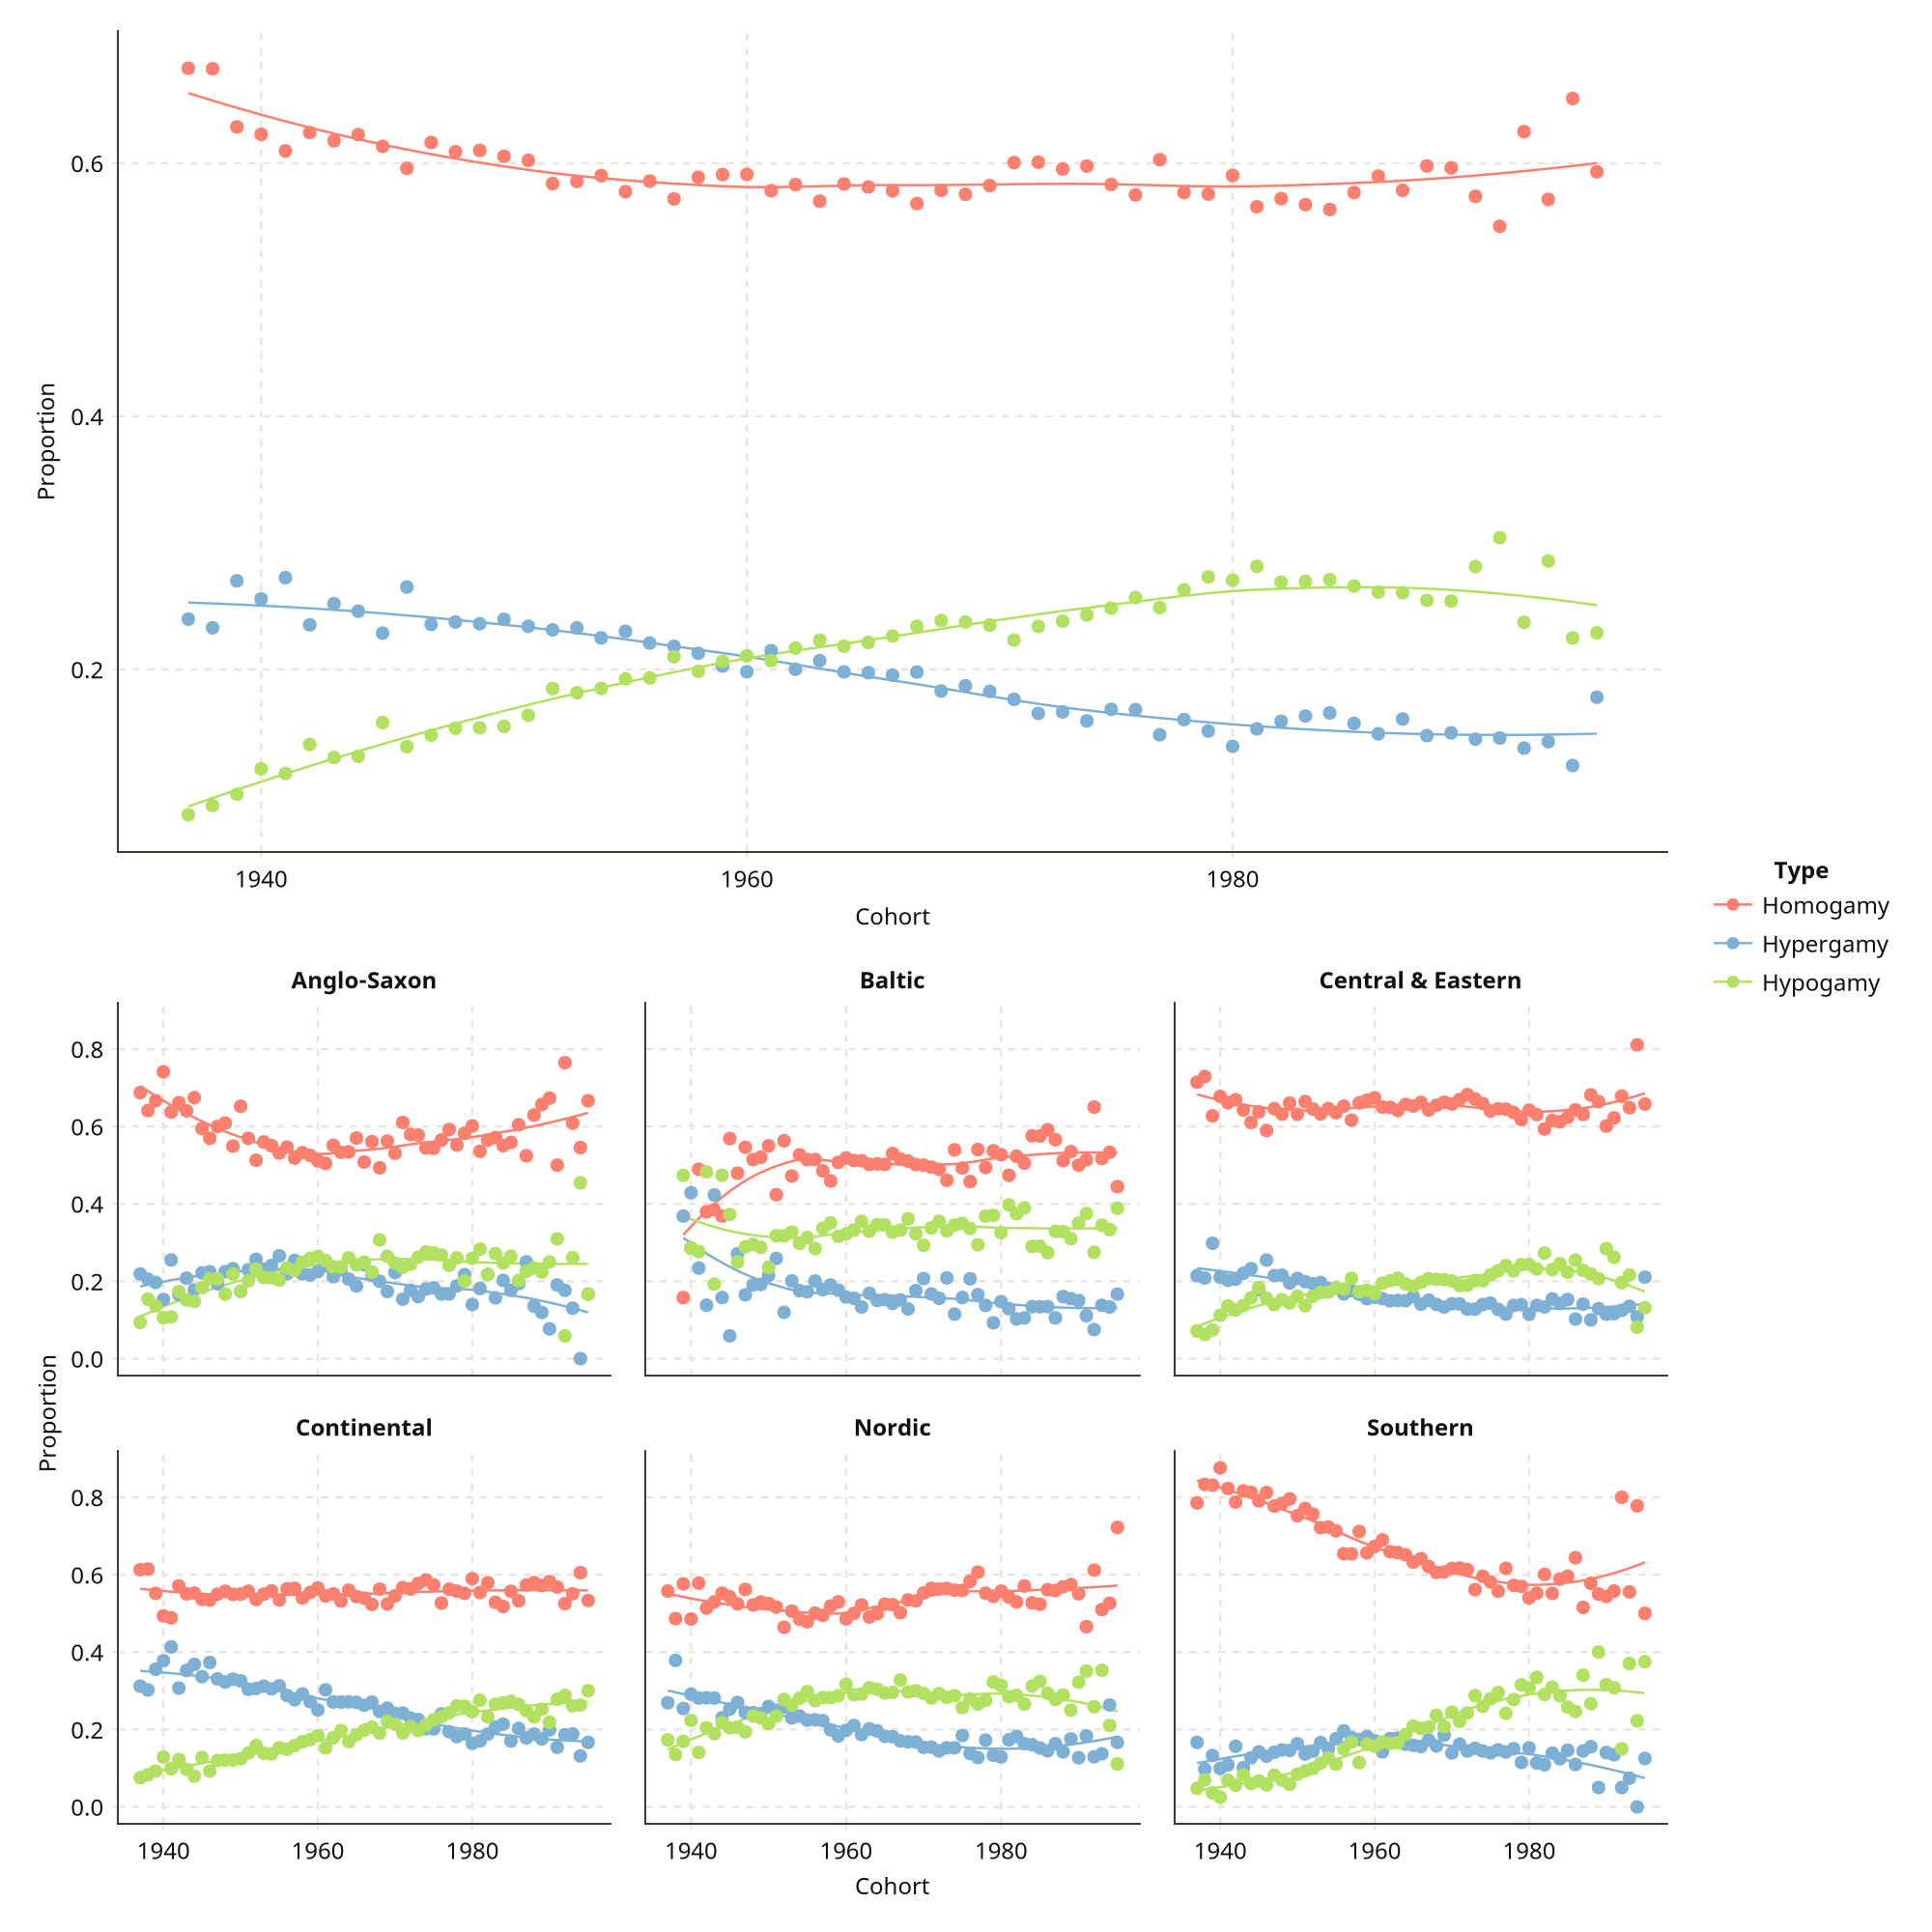
\includegraphics[width=0.9\textwidth]{chapters/chapter3/figures/trends.png}
    \caption{Trends in educational sorting patterns.}
    \label{fig:trends_edu_sorting}
\end{figure}

\begin{figure}[H]
    \centering
    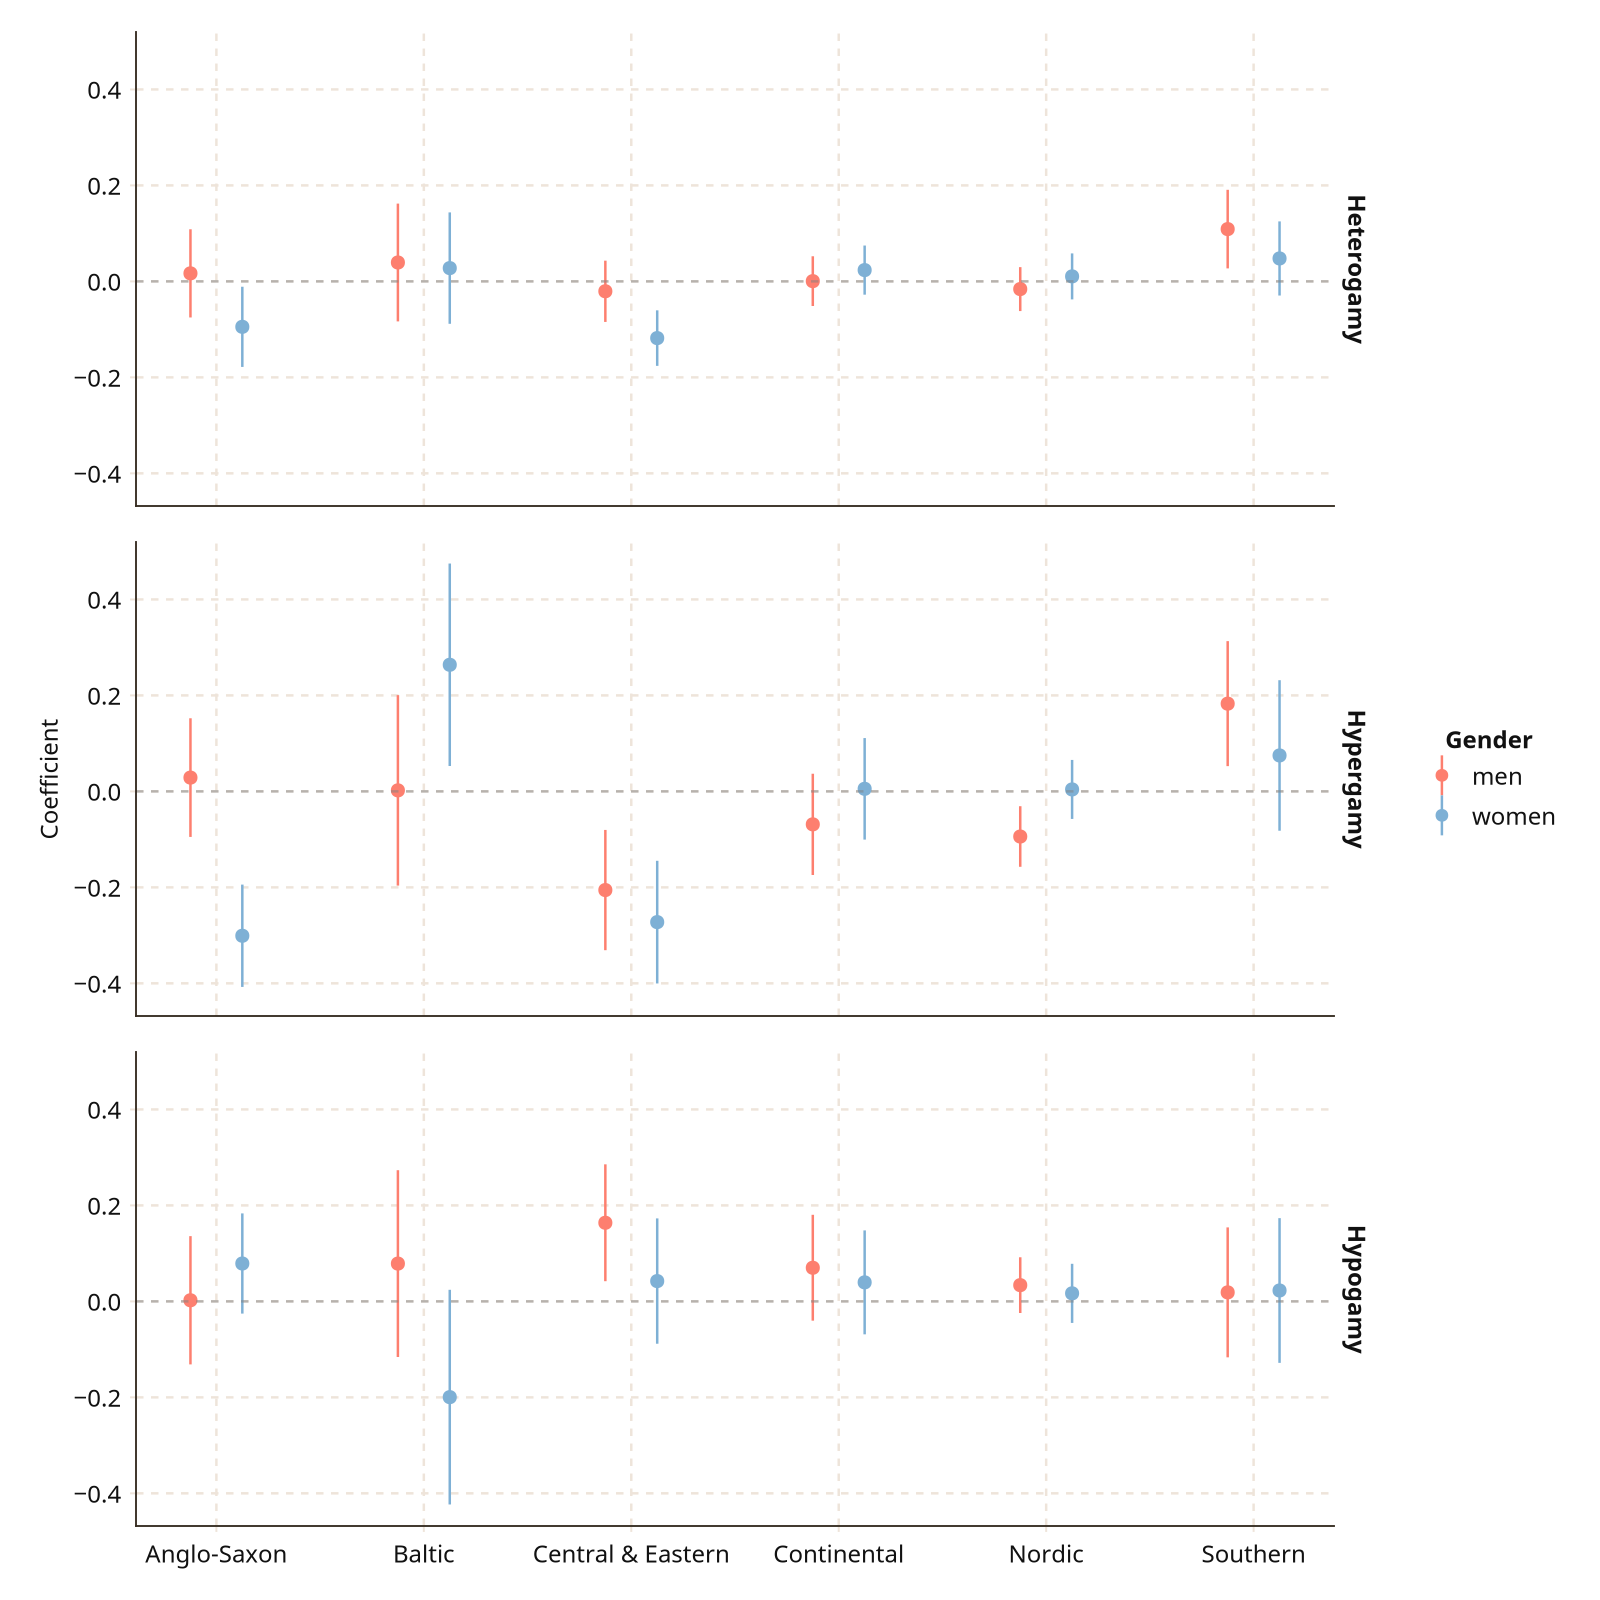
\includegraphics[width=0.9\textwidth]{chapters/chapter3/figures/dmm_region.png}
    \caption{Educational sorting and life satisfaction across country clusters.}
    \label{fig:dmm_region}
\end{figure}

\chapter{Understanding Trends in Educational Sorting in Marriage}
\label{chap:explain-edu-sorting}

% Input individual section files
\section{Introduction}
\label{sec:ch4-introduction}

Trust, "one of the most important synthetic forces within society," is vital for establishing and maintaining meaningful relationships \parencite[p.~326]{simmelSociologyGeorgSimmel1964}. Trust enables us to develop secure attachments with those close to us and to exchange information and cooperate with those more distant \parencite{rusbultCommitmentTrustClose1999,schilkeTrustSocialRelations2021,simpsonFoundationsInterpersonalTrust2007}. Within the larger society, trust, a core component of social capital, fosters inclusiveness, civic engagement, and collective actions, all of which are foundational for economic, democratic, and cultural prosperity \parencite{fukuyamaTrustSocialVirtues1996,fukuyamaSocialCapitalCivil2001,putnamBowlingAloneCollapse2001}.

Since \citeauthor{easterlinDoesEconomicGrowth1974}'s (\citeyear{easterlinDoesEconomicGrowth1974}) pioneering work, individuals' subjective well-being, the subjective experience and evaluation of various domains of life, has garnered considerable research attention. Trust plays a prominent role in this context, at times even surpassing the importance of income \parencite{bjornskovHappyFewCross2003,helliwellHowsLifeCombining2003}. Numerous studies in both developed and developing societies have demonstrated that individuals with a higher level of trust are happier \parencite{luLongitudinalEvidenceSocial2019,rodriguez-poseSocialCapitalIndividual2013}, more satisfied with life \parencite{zhangSocialTrustSatisfaction2020}, and exhibit fewer depressive symptoms \parencite{fahmiDoesYourNeighborhood2019,fujiwaraProspectiveStudyIndividuallevel2008}. The benefits of trust extend to collectives as well; those residing in communities or nations with higher aggregated levels of trust have better overall well-being, controlling for their own level of trust \parencite{helliwellHowsLifeCombining2003,tovWellBeingNationsLinking2009}.

Nevertheless, there has been a lack of consensus on what trust, an inherently multidimensional and multifaceted construct, designates across contexts \parencite{nannestadWhatHaveWe2008}. Previous studies on social capital have often used generalized trust to represent a moralized belief in human goodness \parencite{adedejiExaminingPathwaysGeneral2023,helliwellHowsLifeCombining2003,helliwellSocialContextWell2004}. However, given strong familism and limited civic participation in China, scholars have questioned whether generalized trust is as significant for subjective well-being in China as it is in Western societies, and whether it can be accurately measured by the standard survey item: “Generally speaking, would you say that most people can be trusted or that you need to be very careful in dealing with people” \parencite{delheyHowGeneralTrust2011,liParticularizedTrustGeneralized2002}. In societies where the trust radius—the maximum distance between the subject and objects of trust—is narrow, respondents, when asked about "most people," may draw on relationships within their immediate circles of contacts rather than the general population \parencite{liParticularizedTrustGeneralized2002}. Consequently, responses may misidentify particularized trust in known, familiar individuals as the intended generalized trust, obscuring scholars from estimating how various types of trust affect subjective well-being.

Therefore, the first contribution of this study is to contextualize trust in the Chinese context by distinguishing between generalized and particularized trust and investigating their well-being implications separately. For more precise measures, I employ survey items that clearly specify the objects of trust within and beyond the trust radius for measuring particularized and generalized trust, respectively.

Trust is not only a multidimensional construct but also a relational one \parencite{lewisTrustSocialReality1985}. However, previous literature, primarily focusing on individuals or collectives as units of analysis, have offered limited evidence on how one person's trust may extend its benefits to others, especially their close ones, via relational pathways. Viewing trust as a relational construct within family systems \parencite{bowenUseFamilyTheory1966}, this study explores the dyadic spillover effects of trust in marital relationships, where husbands and wives are interdependent and mutually influential, and trust, especially particularized trust, may extend its benefits beyond the individual to influence their spouse's subjective well-being. The focus on married couples is twofold: not only does the prevalence and centrality of marriage in China make this study relevant to a large demographic \parencite{jiangMarriageSqueezeNeverMarried2014,yanChineseFamiliesUpside2021}, but marital relationships also serve as a primary locus for observing the gendered power dynamics embedded in husband-wife interactions \parencite{barberLogicLimitsTrust1983,jiUnequalCareUnequal2017}. Given the persistent male-husband-father supremacy, I anticipate that husbands' trust will have a greater impact on couple' subjective well-being than wives' trust.

This study further contributes to the literature by examining the relational pathways through which trust influences individuals' and their spouse's well-being. Previous research on intimate relationships has found that trust improves relational satisfaction and broadens interpersonal relationships, which are integral to subjective well-being \parencite{adilRoleTrustMarital2013,fitzpatrickAttachmentTrustSatisfaction2017,luLongitudinalEvidenceSocial2019,shekMaritalQualityPsychological1995,wongExaminationRelationshipTrust2002}. Building on this line of literature, I explore the relational pathways—marital satisfaction and interpersonal relationships—as mediating mechanisms that could explain the well-being implications of trust on both the individual and dyadic levels.

To this end, this study utilizes a lagged Actor-Partner Interdependence Model with Mediation (APIMeM) to assess how generalized and particularized trust influences married couples' subjective well-being across multiple domains, including life satisfaction, happiness, and depression, with attention to gender variations and the relational pathways mediating these associations. The lagged APIMeM is a dyadic and longitudinal approach that isolates and estimates the within- and between-individual influence of trust, while controlling for intra-couple covariances in trust and subjective well-being. It also reduces biases caused by omitted variables by holding constant the baseline well-being outcomes. I selected a nationally representative sample of 6,694 pairs of heterosexual married couples from the China Family Panel Studies in 2014 and 2018.

The article is organized as follows. I start with the conceptualization and measures of trust in the Chinese context, followed by a brief review of empirical evidence on the well-being implications of trust. Next, I contextualize trust within marital relationships, with a focus on gender dynamics and relational mechanisms. Subsequently, I present the data, methods, and findings. I conclude by summarizing findings and discussing limitations and future implications.

\section{Theoretical Framework}
\label{sec:ch4-theoretical-framework}

\subsection{Trust in the Chinese Context}

\subsubsection{Conceptualizing Trust: Generalized and Particularized Trust}

Trust is a multidimensional construct with varying meanings across contexts. As \textcite{barberLogicLimitsTrust1983}noted, the meanings of trust are socially learned and cannot be isolated from the social environment and culture within a specific context. Therefore, it is crucial to clarify the types of trust considered in this study before examining their well-being implications.

In Chinese society characterized by strong familism, trust is viewed as being intrinsically linked to and strictly confined within familial relationships and kinship networks \parencite{weberReligionChinaConfucianism1968,yanIntergenerationalIntimacyDescending2016,yanChineseFamiliesUpside2021}. Therefore, this type of trust cannot be generalized to those outside blood-tied communities. Some scholars, like \textcite{fukuyamaTrustSocialVirtues1996}, have argued that familial societies, such as China and Italy, lack the soil for fostering trust towards strangers and the general population.

However, this narrow view of strictly kinship-based trust has been challenged. \textcite{feiSoilFoundationsChinese1992}, in his seminal work From the Soil, introduced the "patterns of difference (\textit{chaxugeju})," likening interpersonal relationships (\textit{guanxi}) in China to ripples forming and spreading across the surface of a lake. As the ripple moves further outward, it diminishes and eventually becomes insignificant to the individual at the center. This analogy vividly illustrates that trust may extend beyond kinship networks through interpersonal relationships, though it wanes and eventually dissolves as it approaches the "trust radius"—the maximum distance between the subject and objects of trust \parencite{liParticularizedTrustGeneralized2002}.

Over recent decades, China's marketization and modernization have somewhat diminished familism and fostered socioeconomic conditions supportive of trust towards the general population \parencite{xuChangesMainlandChinese2014,yanChineseFamiliesUpside2021}. Dramatic social changes, including rapid urbanization, educational expansion, and the emerging civil sector, have broadened individuals' interactions between their immediate social circles \parencite{bianOccupationClassSocial2005,steinhardtSocioEconomicModernizationCrisis2020}. These social changes have catalyzed a modern society, where the development of a moralized, unconditional trust in others becomes possible.

Against this backdrop, this study distinguishes two types of trust in China. On one end of the spectrum is particularized trust on known, familiar individuals within one's immediate social circles \parencite{delheyHowGeneralTrust2011,kramerIngroupOutgroupTrust2017,steinhardtSocioEconomicModernizationCrisis2020}. This form of trust is confined within the limits of interpersonal relationships and rarely extends beyond the trust radius. At the other end lies generalized trust, also known as thick, diffuse, or moralized trust, which reflects an overarching belief in the "the benevolence of human nature \parencite[p.~139]{yamagishiTrustCommitmentUnited1994}." Unlike particularized trust, generalized trust is not reliant on personal interactions and encompasses strangers and the general population.

\subsubsection{Measuring Generalized and Particularized Trust}

Generalized trust is often measured by the standard survey question: "Generally speaking, would you say that most people can be trusted or that you need to be very careful in dealing with people?" \parencite{rosenbergMisanthropyPoliticalIdeology1956}. Adopted from the American General Social Surveys to many cross-national surveys like the World Value Survey (WVS) and the European Social Survey (ESS), this survey item has gained popularity for it has a very low non-response rate and remains remarkably consistent over time within the same country \parencite{nannestadWhatHaveWe2008}. However, its validity and accuracy in non-Western contexts, especially in East Asia, have been increasingly challenged \parencite{delheyPredictingCrossNationalLevels2005,glaeserMeasuringTrust2000,torpeIdentifyingSocialTrust2011}. Given the ambiguity of "most people," respondents must rely on their own interpretations and give responses to whether they trust individuals within their "trust radius." Consequently, when the trust radius is narrow, the survey question may incorrectly identify particularized trust as generalized trust, making this measure difficult to compare across contexts \parencite{delheyHowGeneralTrust2011,delheyPredictingCrossNationalLevels2005,torpeIdentifyingSocialTrust2011}.

The trust radius in China remains relatively narrow. An earlier study found that the subjects of "most people" rarely extended beyond the immediate circles of contacts, such as family members, neighbors, and intimate friends \parencite{liParticularizedTrustGeneralized2002}. More recent cross-national studies calculated the trust radius as the correlations between trust toward specified in-group and out-group members, ranking China 47th out of 51 countries surveyed \parencite{delheyHowGeneralTrust2011}. These findings suggest that the standard survey item, with unspecified targets of trust, may not effectively capture the nuances of trust dynamics within the Chinese context.

Considering these concerns, it is important to use alternative survey items sensitive to the trust radius when measuring generalized and particularized trust. This study employs survey items that clearly define the targets of trust to ensure more accurate measures: individuals within close relationships (e.g., family members, neighbors) for particularized trust and those beyond the trust radius (e.g., strangers) for generalized trust.

\subsection{Trust and Couples' Subjective Well-Being}

\subsubsection{Trust as a Strong Determinant of Individual's Well-Being}

Generalized trust, when measured towards the unspecific "most people," is often regarded as one of the strongest determinant of individuals' subjective well-being \parencite{adedejiExaminingPathwaysGeneral2023,helliwellHowsLifeCombining2003}. However, when measured towards strangers or out-group members, findings appear to be more contentious. Several studies reported that individuals with higher levels of trust in strangers were happier, more satisfied with life, and exhibit fewer depressive symptoms \parencite{churchillTrustSocialNetworks2017,baiSocialTrustPattern2019}, whereas other research found no significant associations between trust towards out-group members and self-rated health in China, Japan, and Korea \parencite{sungTrustHealthCrossnational2019,sungIngroupTrustSelfrated2020}. One study in South Africa suggested that trust in strangers did not yield benefits, but instead led to worsened depressive symptoms \parencite{adjaye-gbewonyoHighSocialTrust2018}.

Empirical evidence on the well-being implications of particularized trust is more consistent across contexts. Utilizing data from the WVS, \textcite{sungTrustHealthCrossnational2019} found almost universal positive associations between trust towards in-group members and self-rated health worldwide. In East Asia, \textcite{sungIngroupTrustSelfrated2020} observed benefits of trust towards in-group members in all four regions surveyed (China, Korea, Japan, and Taiwan), whereas the positive influence of out-group trust on health was significant only in Taiwan. However, exceptions do exist. For instance, \textcite{baiSocialTrustPattern2019} found that in China, individuals' happiness was positively associated with generalized trust toward strangers but unaffected by trust in family members.
Considering these findings, I propose the following hypotheses at the individual level.

\begin{quote}
    \textbf{H1a.} Generalized trust is positively associated with individuals' life satisfaction and happiness, and negatively associated with depression.

    \textbf{H1b.} Particularized trust is positively associated with individuals' life satisfaction and happiness, and negatively associated with depression.
\end{quote}

\subsubsection{Contextualizing Trust in Marriage: The Spillover Effects of Trust}

Despite abundant evidence on the individual- and contextual-level outcomes of trust, there has been limited research on how trust functions within relationships, specifically, how one person's trust may extend its benefits to others via relational pathways. The current study shifts the perspective from viewing trust as merely an individualistic attribute to emphasizing its relational nature and contextualizing it within dyadic interactions. Specifically, I focus on marital relationships, in which individuals' trust may not only influence their own subjective well-being but also spill over to impact their spouse's.

I focus on husband-wife dyads for several reasons. First, marriage remains one of the most prevalent and salient relationships in China \parencite{jiangMarriageSqueezeNeverMarried2014,yanChineseFamiliesUpside2021}. Despite declining marriage rates, China is still characterized by universal marriage and traditional familial values \parencite{jiHeterogeneityContemporaryChinese2014}. Fewer than 5\% of women and 10\% of men remained single by the age of 30 to 34, and the percentage of the lifelong single population has consistently stayed below 5\% \parencite{jiangMarriageSqueezeNeverMarried2014}. Therefore, focusing on husband-wife dyads allows the findings of the present study to be generalizable to a large demographic.

Second, marriage provides a unique context where trust has both individual- and dyadic-level ramifications for couples' subjective well-being. Drawing from \citeauthor{bowenUseFamilyTheory1966}'s \citeyear{bowenUseFamilyTheory1966} family system theory, we view family as a social system and emotional unit, where family members are interdependent and mutually influential. This theory underpins the relational nature of trust within dyadic relationships, where not only is there an intra-couple correlation in trust and well-being, but the trust of one partner may also spill over to influence the other's well-being. Similar dyadic interactions with regard to other spousal characteristics have been observed, such as the negative effects of husband's role strain on their own and their spouse's marital satisfaction \parencite{brockLongitudinalInvestigationStress2008} and the associations between individuals' reemployment and couples' well-being \parencite{scheuringDoesFixedTermEmployment2021}. This study extends this line of literature to examine the individual- and dyadic-level implications of trust for couples' subjective well-being.

Third and lastly, marriage serves as the primary locus exhibiting gendered power dynamics embedded in husband-wife interactions. "A basic fact about family trust," stated by \textcite[p~27]{barberLogicLimitsTrust1983}, "is male-husband-father supremacy, which extends over the wife and the children." This is especially pronounced in the Chinese context, where scholars have observed a resurgence of patriarchal values in recent decades \parencite{jiUnequalCareUnequal2017}. It is, therefore, likely that characteristics of the husband, including levels of trust, predominantly influence couples' subjective well-being, outweighing those of the wife.

Due to the strong relevance of particularized trust to intimate relationships within the trust radius, I anticipate that particularized trust will exert a dyadic-level influence on subjective well-being, whereas generalized trust, directed towards strangers or out-group members, is unlikely to extend its benefits beyond individuals themselves. Based on these considerations, I propose the following hypotheses:

\begin{quote}
    \textbf{H2a.} Particularized trust is positively associated with the spouse's life satisfaction and happiness and negatively associated with the spouse's depression, with husbands exerting a greater influence than wives.

    \textbf{H2b.} Generalized trust is not associated with the spouse's life satisfaction and happiness, and not associated with the spouse's depression.
\end{quote}

\subsubsection{The Relational Pathways as Mediating Mechanisms}

Viewing trust as a relational construct, this study further explores the relational pathways through which trust, especially particularized trust, influences individuals' and their spouse's subjective well-being. Previous studies have provided valuable insights on the individual level. \textcite{luLongitudinalEvidenceSocial2019}, featuring a comprehensive mediation analysis, found that social ties accounted for around 10\% of the total effects of generalized trust on individuals' happiness. Other studies indicated that particularized trust towards family members enhances relational satisfaction and strengthens interpersonal relationships, both of which are crucial for subjective well-being \parencite{adilRoleTrustMarital2013,fitzpatrickAttachmentTrustSatisfaction2017,shekMaritalQualityPsychological1995,wongExaminationRelationshipTrust2002}.

This study is concerned with the relational mechanisms mediating the associations between trust and subjective well-being at both the individual and dyadic levels. Specifically, I identify marital satisfaction and interpersonal relationships as two key mediators that could explain these associations. This leads to the third hypothesis:

\begin{quote}
    \textbf{H3.} Marital satisfaction and interpersonal relationships mediate the associations between trust and couples' subjective well-being.
\end{quote}

\section{Data and Methods}
\label{sec:ch4-data-methods}

% Your data and methods content will go here 
\section{Results}
\label{sec:ch4-results}

% Your results content will go here 
\section{Discussion}
\label{sec:ch4-discussion}

Using data from China's Census, our study examined trends in marital sorting outcomes by education across consecutive cohorts born between 1946 and 1985. We first described how the prevalence of homogamy, hypergamy, and hypogamy varied across cohorts and urban/rural regions, and how the three driving forces (i.e., educational expansion, gender- and education-specific marriage rates, assortative mating preferences) shifted correspondingly. We then employed a decomposition approach to disentangle the respective contributions of these three factors to the observed educational sorting outcomes in marriage.

Our descriptive findings align with previous studies in China \parencite{dongTrendsEducationalAssortative2023,hanTrendsEducationalAssortative2010,shiSevenDecadesEducational2019}. Specifically, we observed a U-shaped curve for homogamy, an inverted U-shaped curve for hypergamy, and an initial rise in hypogamy followed by stagnation. Throughout the course of educational expansion, the educational composition within both the married population and the general population has become more heterogeneous within each gender but more homogeneous between genders \parencite{yeungHigherEducationExpansion2013}. Changes in educational structure could have led to a substantial increase in hypogamy, as seen in other contexts, if not for the rapidly declining marriage rates among highly educated women and the intensified assortative mating preferences against heterogamy, especially hypogamy \parencite{hanTrendsEducationalAssortative2010,huGenderEducationExpansion2023}. These unique dynamics highlight the intricate interplay between tradition and modernity in China, reflected in the co-existence of both rejection and adherence to traditional marriage norms: the higher a woman's educational attainment, the less likely she is to marry; but if she does, the less willing she is to marry downwards.

Applying the decomposition approach proposed by \textcite{leeschDecomposingTrendsEducational2023}, we quantitatively explained why these trends occurred in China, a transitional country with rapid but uneven development over the past century. Our decomposition results show that the initial decline in homogamy and the corresponding increase in heterogamy across cohorts born before 1965 were driven entirely by educational expansion, while the gender-education-specific marriage rates and assortative mating preferences played negligible roles. For later birth cohorts, sustained educational expansion—characterized by a further convergence of gender education gaps—promoted homogamy and hypogamy while discouraging hypergamy, outweighing the opposing force of a steeper decline in marriage rates among highly educated women. These cohorts also exhibited intensified preferences for homogamy and against heterogamy. These three factors jointly explained the patterns of increasing homogamy, declining hypergamy, and stagnant hypogamy among later birth cohorts.

These results differ from those found by \textcite{leeschDecomposingTrendsEducational2023} in Ireland, where, in addition to educational expansion, the increasing marriage rates among highly educated women contributed to rising homogamy and declining hypergamy, whereas the impact of assortative mating preferences were minimal. These differences suggest that the unique demographic transitions and the unparalleled importance of education in shaping China's sociodemographic changes contributed to the complex dynamics among structural conditions, marriage rates, and assortative mating preferences.

Unexpectedly, the urban-rural differences in marital sorting outcomes by education have been narrowing across cohorts born between 1966 and 1985. Furthermore, upon decomposing the differences across urban and rural regions, we found that a steeper decline in marriage rates among highly educated women in rural regions was a significant force narrowing the urban-rural gap in homogamy. Regarding heterogamy, diminishing differences in the impact of educational expansion were the main contributor to this convergence. Among younger cohorts born between 1981 and 1985, the rates of hypergamy converged across urban and rural areas, and the remaining differences in hypogamy were largely due to educational structures and stronger assortative mating preferences against hypogamy in rural areas. Those findings suggest that, despite the persistent socioeconomic disparities, marriage was one of the primary sites where the integration of urban and rural China took place.

This study, however, is not without limitations. First, the decomposition approach, in its strict form, assumes that educational expansion, education-specific marriage rates, and assortative mating preferences are independent forces \parencite{leeschDecomposingTrendsEducational2023}. This assumption may not hold in reality, as the expansion of higher education could marginalize certain groups, particularly less-educated men, further squeezing them out of the marriage market and, in turn, affecting the educational gradients in marriage rates \parencite{jiangMarriageSqueezeNeverMarried2014}. Similarly, assortative mating preferences may shift due to the increasing prominence of education during periods of educational expansion. Nevertheless, this limitation is common in other analyses using the decomposition or log-linear approach and does not weaken the strength of our study in distinguishing the respective contributions of the three aforementioned factors.

Second, our study is limited by the exclusion of marriages between spouses with different \textit{hukou} statuses. We excluded this group for analytical reasons. However, this is a very selective group, representing less than 5\% of all marriages across cohorts in our sample \parencite{duTrendsEducationalAssortative2023}. Moreover, as mentioned earlier, \textit{hukou} conversion often requires stringent conditions. Therefore, we do not think this decision will affect the results significantly. Still, we want to note that our findings on the diminishing urban-rural gaps in marital sorting by education are limited to spouses who share the same \textit{hukou} status.

Third, the four-level education may obscure stratification mechanisms within each level \parencite{fengRevisitingHorizontalStratification2022}. At the lower end of the spectrum, illiteracy and primary school education were grouped together, meaning marriages between individuals with these two statuses were classified as homogamous. Likewise, vocational colleges, which have become more prevalent among younger cohorts, are often considered inferior to four-year colleges due to their less stringent entry requirements and lower socioeconomic returns. To ensure a sizable population within each level across cohorts, we were unable to utilize finer educational gradients. Furthermore, as aforementioned, this categorization is still effective in capturing varied socioeconomic returns in contemporary China.

Lastly, the census data did not include information on cohabitation, which limited our ability to account for educational sorting outcomes in this relationship. However, this is unlikely to significantly affect our results, as cohabitation remains uncommon and is largely viewed as a predecessor to marriage in China \parencite{muChangingPatternsDeterminants2022}.

These limitations do not diminish the strength of our study. To the best of our knowledge, this is the first study to systematically account for both preferences and structural conditions in understanding variations in educational sorting outcomes in marriage across cohorts and between urban and rural areas in China. Additionally, we captured structural influences within both the married and the general population, providing novel evidence on how marriage plays a role in the nuanced implications of modernization. Despite various changes, the dominance of homogamy may further intensify social stratification. While some highly educated women depart from traditional gendered marital norms by opting out of marriage, those who do marry tend to adhere more strongly to hypergamy than their less educated counterparts. Surprisingly, despite the widened urban-rural socioeconomic disparities, patterns of marital sorting in urban and rural China are converging, highlighting the pervasiveness of changing family ideals and forms. We encourage further research to extend this line of inquiry to other contexts and through a cross-national perspective.


% Input tables and figures
% Descriptive statistics of the sample
\begin{table}[H]
    \caption{Descriptive Statistics}
    \label{tab:trust-descriptive-stats}
    \setlength{\tabcolsep}{1.0em}
    \renewcommand{\arraystretch}{1.1}
    \begin{tabularx}{\textwidth}{@{} l|*{3}{>{\centering\arraybackslash}X} @{}}
        \hline
                                    & Men           & Women         & T-Test    \\
        \hline
        Life satisfaction           & 4.09 (0.92)   & 4.11 (0.94)   & -1.41     \\
        Happiness                   & 7.63 (2.05)   & 7.59 (2.14)   & 0.90      \\
        Depression                  & 31.67 (7.41)  & 33.83 (7.99)  & -16.57*** \\
        Generalized trust           & 2.08 (2.09)   & 1.74 (2.06)   & 9.82***   \\
        Particularized trust        & 8.13 (140)    & 7.97 (1.48)   & 6.51***   \\
        Marital satisfaction        & 4.68 (0.66)   & 4.43 (0.88)   & 19.18***  \\
        Interpersonal relationship  & 7.13 (1.92)   & 7.21 (2.00)   & -2.42*    \\
        Age                         & 49.24 (12.87) & 47.38 (12.63) & 8.60***   \\
        Number of children          & 1.38 (0.89)   & 1.38 (0.89)   & --        \\
        Household income per capita & 13035 (18925) & 13035 (18925) & --        \\
        Education (years)           & 8.03 (4.05)   & 6.35 (4.68)   & 22.66***  \\
        Marriage duration (years)   & 25.30 (13.04) & 25.30 (13.04) & --        \\
        \hline
    \end{tabularx}
    \begin{flushleft}
        \small
        \textit{Note:} Standard deviations are presented in parentheses. Between-gender differences are assessed by T-tests. Data includes 6,964 pairs of married couples selected from the China Family Panel Studies in 2014 and 2018.
    \end{flushleft}
\end{table}

% APIMs on Couples' Subjective Well-Being
\begin{table}[H]
    \caption{APIMs on Couples' Subjective Well-Being}
    \label{tab:apim-results}
    \setlength{\tabcolsep}{1.0em}
    \renewcommand{\arraystretch}{1.2}
    \begin{tabularx}{\textwidth}{@{} l|*{3}{>{\centering\arraybackslash}X} @{}}
        \hline
                                        & Life satisfaction & Happiness & Depression \\
        \hline
        \multicolumn{4}{l}{\textit{Particularized trust}}                            \\
        Actor (men$\rightarrow$men)     & 0.06***           & 0.06***   & -0.11***   \\
        Actor (women$\rightarrow$women) & 0.05**            & 0.02      & -0.07***   \\
        Partner (women$\rightarrow$men) & 0.02              & 0.03      & -0.03*     \\
        Partner (men$\rightarrow$women) & 0.03*             & 0.04**    & -0.04**    \\
        \multicolumn{4}{l}{\textit{Generalized trust}}                               \\
        Actor (men$\rightarrow$men)     & -0.00             & -0.00     & -0.04**    \\
        Actor (women$\rightarrow$women) & -0.00             & -0.02     & -0.00      \\
        Partner (women$\rightarrow$men) & 0.01              & -0.00     & 0.00       \\
        Partner (men$\rightarrow$women) & -0.00             & 0.01      & -0.01      \\
        \hline
    \end{tabularx}
    \begin{flushleft}
        \small
        \textit{Note:} Data includes 6,964 pairs of married couples selected from the China Family Panel Studies in 2014 and 2018.
    \end{flushleft}
\end{table}

% APIMeMs on Couples' Subjective Well-Being Mediated by Marital Satisfaction
\begin{table}[H]
    \caption{APIMeMs on Couples' Subjective Well-Being Mediated by Marital Satisfaction}
    \label{tab:apimem-ms-results}
    \setlength{\tabcolsep}{1.0em}
    \renewcommand{\arraystretch}{1.2}
    \begin{tabularx}{\textwidth}{@{} l|*{3}{>{\centering\arraybackslash}X} @{}}
        \hline
                                           & Life Satisfaction & Happiness & Depression \\
        \hline
        \multicolumn{4}{l}{\textit{Particularized trust}}                               \\
        Actor effect                       & 0.05***           & 0.04***   & -0.10***   \\
        \hspace{0.5cm}Indirect effect (IE) & 0.02***           & 0.01***   & -0.02***   \\
        \hspace{1cm}Actor-actor IE         & 0.01***           & 0.01**    & -0.02***   \\
        \hspace{1cm}Partner-partner IE     & 0.00*             & 0.00*     & -0.04***   \\
        \hspace{0.5cm}Direct effect        & 0.04***           & 0.03**    & -0.07***   \\
        Partner effect                     & 0.02*             & 0.03***   & -0.04***   \\
        \hspace{0.5cm}Indirect effect (IE) & 0.01***           & 0.01**    & -0.02***   \\
        \hspace{1cm}Actor-partner IE       & 0.00***           & 0.00**    & -0.01***   \\
        \hspace{1cm}Partner-actor IE       & 0.01**            & 0.01*     & -0.01***   \\
        \hspace{0.5cm}Direct effect        & 0.01              & 0.03**    & -0.02*     \\
        \multicolumn{4}{l}{\textit{Generalized trust}}                                  \\
        Actor effect                       & -0.00             & -0.02     & -0.01      \\
        \hspace{0.5cm}Indirect effect (IE) & 0.01              & -0.01**   & 0.00       \\
        \hspace{1cm}Actor-actor IE         & -0.01             & -0.01**   & 0.00*      \\
        \hspace{1cm}Partner-partner IE     & 0.00              & 0.00      & -0.00      \\
        \hspace{0.5cm}Direct effect        & 0.00              & -0.01     & -0.02      \\
        Partner effect                     & 0.00              & -0.00     & 0.00       \\
        \hspace{0.5cm}Indirect effect (IE) & 0.00              & -0.00     & 0.00       \\
        \hspace{1cm}Actor-partner IE       & -0.00             & -0.00**   & 0.00*      \\
        \hspace{1cm}Partner-actor IE       & 0.00              & 0.00      & -0.00      \\
        \hspace{0.5cm}Direct effect        & 0.00              & -0.00     & -0.00      \\
        \hline
    \end{tabularx}
    \begin{flushleft}
        \small
        \textit{Note:} Data includes 6,964 pairs of married couples selected from the China Family Panel Studies in 2014 and 2018.
    \end{flushleft}
\end{table}

% APIMeMs on Couples' Subjective Well-Being Mediated by Interpersonal Relationships
\begin{table}[H]
    \caption{APIMeMs on Couples' Subjective Well-Being Mediated by Interpersonal Relationships}
    \label{tab:apimem-ir-results}
    \setlength{\tabcolsep}{1.0em}
    \renewcommand{\arraystretch}{1.2}
    \begin{tabularx}{\textwidth}{@{} l|*{3}{>{\centering\arraybackslash}X} @{}}
        \hline
                                           & Life Satisfaction & Happiness & Depression \\
        \hline
        \multicolumn{4}{l}{\textit{Particularized trust}}                               \\
        Actor effect                       & 0.05***           & 0.04***   & -0.10***   \\
        \hspace{0.5cm}Indirect effect (IE) & 0.02***           & 0.04***   & -0.02***   \\
        \hspace{1cm}Actor-actor IE         & 0.02***           & 0.03***   & -0.01***   \\
        \hspace{1cm}Partner-partner IE     & 0.00**            & 0.00**    & -0.00**    \\
        \hspace{0.5cm}Direct effect        & 0.04***           & 0.00      & -0.07***   \\
        Partner effect                     & 0.02*             & 0.04***   & -0.04***   \\
        \hspace{0.5cm}Indirect effect (IE) & 0.01***           & 0.02***   & -0.01***   \\
        \hspace{1cm}Actor-partner IE       & 0.00***           & 0.00**    & -0.05***   \\
        \hspace{1cm}Partner-actor IE       & 0.01**            & 0.02***   & -0.01***   \\
        \hspace{0.5cm}Direct effect        & 0.01              & 0.02      & -0.03**    \\
        \multicolumn{4}{l}{\textit{Generalized trust}}                                  \\
        Actor effect                       & -0.00             & -0.02     & -0.01      \\
        \hspace{0.5cm}Indirect effect (IE) & 0.01**            & 0.01*     & -0.00**    \\
        \hspace{1cm}Actor-actor IE         & 0.00**            & 0.01*     & -0.00**    \\
        \hspace{1cm}Partner-partner IE     & 0.00              & 0.00      & -0.00      \\
        \hspace{0.5cm}Direct effect        & -0.01             & -0.03**   & -0.01      \\
        Partner effect                     & 0.00              & -0.00     & 0.00       \\
        \hspace{0.5cm}Indirect effect (IE) & 0.00              & 0.00      & -0.00      \\
        \hspace{1cm}Actor-partner IE       & 0.00*             & 0.00      & -0.00*     \\
        \hspace{1cm}Partner-actor IE       & 0.00              & 0.00      & -0.00      \\
        \hspace{0.5cm}Direct effect        & 0.00              & -0.01     & 0.00       \\
        \hline
    \end{tabularx}
    \begin{flushleft}
        \small
        \textit{Note:} Data includes 6,964 pairs of married couples selected from the China Family Panel Studies in 2014 and 2018.
    \end{flushleft}
\end{table}

% Figures for Chapter 1
% Add your figures here using the figure environment
% Example:
%
% \begin{figure}[htbp]
%     \centering
%     \includegraphics[width=0.8\textwidth]{chapters/chapter1/figures/your-figure}
%     \caption{Your figure caption}
%     \label{fig:ch1-example}
% \end{figure} 
\chapter{Conclusion}
\label{chap:conclusion}

One of the foremost concerns today is the growing inequality in nearly all aspects of life. This is alarming not only in developed countries, but also in developing countries like China, where various forms of inequality, whether by gender, education, ethnicity, health, or well-being, that were once byproducts of the bygone burgeoning economy, have now become its haunting aftermath \parencite{sicularUrbanRuralIncomeGap2007,xieIncomeInequalityTodays2014,yeungHigherEducationExpansion2013}. Boundaries across social groups are becoming increasingly difficult to cross, and gender relations have backslidden due to the resurgence of patriarchal values \parencite{jiUnequalCareUnequal2017}. Perhaps no other institution has experienced these repercussions more profoundly than families, and none other than families, through evolving patterns of union formation, reproduction, and relationship dynamics, holds greater potential as sources of social change.

The above chapters have illustrated this point through addressing how individuals and their family members' well-being is impacted by three important family-related and relationship-oriented factors: intergenerational mobility, educational sorting in unions, and trust. Specifically, Chapter~\ref{chap:edu-mobility-swb} has shown that individuals and their parents were not necessarily better off when moving upwards, but both generations' well-being was impaired by downward mobility—a phenomenon observed exclusively among only-child families. I highlight, therefore, the plight of mobility—penalties for falling downwards with no returns to moving upwards—that traps both generations in only-child Chinese families.

Chapter~\ref{chap:edu-sorting-swb} has demonstrated that educational sorting in unions has repercussions on individuals' well-being, with variations between genders and across contexts. Hypergamy (women partnering with more educated men) was the least optimal arrangement for both genders, and men were more satisfied with life when partnering upwards. Notably, hypergamy will become even more unfavorable for women's well-being over time, as its well-being disadvantage is exacerbated in contexts where such partnerships are less normative.

In Chapter~\ref{chap:trust-swb}, I focused on the role of trust in shaping individuals' and their spouse's subjective well-being through relational pathways. I differentiated between generalized and particularized trust, and found that particularized trust, through improving marital satisfaction and interpersonal relationships, significantly enhanced individuals' well-being in all dimensions and extended its benefits from husbands to wives, but not vice versa. Generalized trust, on the other hand, had limited effects and did not spill over. These findings suggest that husband-wife dyadic interactions remain gendered and asymmetric, and that particularized trust is the more effective trust type for improving couples' well-being.

Theoretically, these chapters contribute to the literature by underscoring the importance of embracing the perspective of linked lives, that individuals' well-being is not solely determined by his or her own characteristics, but contingent upon their related ones, and therefore, must be studied \textit{in relation to} others and sensitive of the social context.

Methodologically, this dissertation demonstrates the use of the Diagonal Mobility Models to disentangle the effects of various factors within the stratification-generating mechanisms, as well as the use of the Actor-Partner Interdependence Models to distinguish various relational pathways through which trust enhances well-being. These methods are particularly useful in operationalizing the linked lives' perspective.

Future research may address the limitations of these studies, including but not limited to examining the varying outcomes of educational mobility and sorting across the educational spectrum, addressing the contextual characteristics apart from the normative climate, and incorporating the emerging non-conventional families.


% Bibliography
\begin{sloppypar}
    \printbibliography[heading=bibintoc,title=References]
\end{sloppypar}

% Appendices
\appendix
% Main appendix file that includes all other appendices
\appendix
\chapter{Additional Material}
\label{app:appendices}

% Include individual appendix files
\section{Additional Material for Chapter 2}
\label{app:chapter2}

% Table A1: Steps of sample restriction
\begin{table}[H]
    \caption{Steps of sample restriction.}
    \label{app:tab:sample_restriction_ch2}
    \begin{tabularx}{\textwidth}{@{} l|>{\raggedright\arraybackslash}X|>{\centering\arraybackslash}p{2cm}|>{\centering\arraybackslash}p{2.5cm} @{}}
        \hline
        Step & Sample restriction                       & Parents & Primary Movers \\
        \hline
        0    & Original sample of the CFPS in 2010      & 33,598  & 33,598         \\
        1    & Parents with only one child              & 10,261  &                \\
        2    & Not in school and between ages 20 and 50 & 3836    & 18,172         \\
        3    & Drop those with missing values           & 3808    & 16,385         \\
        \hline
    \end{tabularx}
    \begin{flushleft}
        \small
        \textit{Notes:} Among 16,385 primary movers, 1475 respondents were identified as only children.
    \end{flushleft}
\end{table}

\begin{table}[H]
    \caption{Descriptive statistics of only-children and parents by gender.}
    \label{app:tab:descriptive_by_gender}
    \setlength{\tabcolsep}{0.8em}
    \renewcommand{\arraystretch}{1.2}
    \begin{tabularx}{\textwidth}{@{} l|*{4}{>{\raggedright\arraybackslash}X} @{}}
        \hline
                             & Son          & Daughter     & Father       & Mother       \\
        \hline
        Life satisfaction    & 3.28 (1.07)  & 3.49 (0.92)  & 3.42 (1.08)  & 3.44 (1.03)  \\
        Age                  & 30.16 (7.55) & 30.86 (8.19) & 54.92 (7.86) & 53.34 (7.82) \\
        Minority             & 0.05 (0.21)  & 0.06 (0.24)  & 0.04 (0.20)  & 0.04 (0.20)  \\
        Married              & 0.61 (0.49)  & 0.69 (0.46)  & 0.92 (0.27)  & 0.89 (0.31)  \\
        Party member         & 0.07 (0.26)  & 0.05 (0.23)  & 0.18 (0.39)  & 0.05 (0.23)  \\
        Urban                & 0.69 (0.46)  & 0.73 (0.44)  & 0.67 (0.47)  & 0.69 (0.46)  \\
        Economically related & 0.70 (0.46)  & 0.49 (0.50)  & 0.73 (0.45)  & 0.75 (0.43)  \\
        \textit{Education}   &              &              &              &              \\
        Primary or lower     & 16.88\%      & 20.74\%      & 37.27\%      & 44.42\%      \\
        Middle school        & 31.01\%      & 21.40\%      & 35.47\%      & 32.71\%      \\
        High school          & 22.35\%      & 21.24\%      & 18.88\%      & 18.58\%      \\
        College or above     & 29.76\%      & 36.62\%      & 8.32\%       & 4.29\%       \\
        Total                & 877          & 598          & 1827         & 1981         \\
        \hline
    \end{tabularx}
    \begin{flushleft}
        \small
        \textit{Notes:} Standard deviations are presented in parentheses.
    \end{flushleft}
\end{table}


\section{Additional Material for Chapter 3}
\label{app:chapter3}

% Stepwise sample restrictions
\begin{table}[H]
    \caption{Stepwise sample restrictions}
    \label{app:tab:sample_restriction_ch3}
    \begin{tabularx}{\textwidth}{@{} l|>{\raggedright\arraybackslash}X|>{\centering\arraybackslash}p{2cm} @{}}
        \hline
        Step & Sample restriction                                                                                                & N       \\
        \hline
        0    & Original sample of Rounds 1--10 of the European Social Survey                                                     & 480,625 \\
        1    & Select respondents in marriage or cohabitation with an opposite-sex partner living together in the same household & 271,522 \\
        2    & Select respondents between ages 25 and 65                                                                         & 213,303 \\
        3    & Drop respondents with missing values                                                                              & 195,523 \\
        4    & Drop respondents from countries with less than three rounds of data, and those from Israel                        & 180,733 \\
        \hline
    \end{tabularx}
\end{table}

% Cluster and country information
\begin{table}[H]
    \caption{Cluster, sample size, and survey rounds of each country}
    \label{app:tab:country_clusters}
    \begin{tabularx}{\textwidth}{@{} l|l|>{\centering\arraybackslash}p{2cm}|>{\raggedright\arraybackslash}X @{}}
        \hline
        Cluster            & Country        & N     & Survey rounds                 \\
        \hline
        Anglo-Saxon        & Ireland        & 8710  & 10, 9, 8, 7, 6, 5, 4, 3, 2, 1 \\
                           & United Kingdom & 7525  & 10, 9, 8, 7, 6, 5, 4, 3, 2, 1 \\
        \hline
        Baltic             & Estonia        & 6189  & 10, 9, 8, 7, 6, 5, 4, 3, 2    \\
                           & Lithuania      & 4413  & 10, 9, 8, 7, 6, 5             \\
        \hline
        Central \& Eastern & Bulgaria       & 5525  & 10, 9, 6, 5, 4, 3             \\
                           & Croatia        & 2616  & 10, 9, 5, 4                   \\
                           & Czechia        & 8059  & 10, 9, 8, 7, 6, 5, 4, 2, 1    \\
                           & Hungary        & 6349  & 10, 9, 8, 6, 5, 4, 3, 2, 1    \\
                           & Poland         & 7463  & 9, 8, 7, 6, 5, 3, 2, 1        \\
                           & Russia         & 4600  & 8, 6, 5, 4, 3                 \\
                           & Slovakia       & 4617  & 10, 9, 6, 5, 4, 3, 2          \\
                           & Slovenia       & 5950  & 10, 9, 8, 7, 6, 5, 4, 3, 2, 1 \\
                           & Ukraine        & 3657  & 6, 5, 4, 3, 2                 \\
        \hline
        Continental        & Austria        & 6927  & 9, 8, 7, 5, 4, 3, 2, 1        \\
                           & Belgium        & 7986  & 10, 9, 8, 7, 6, 5, 4, 3, 2, 1 \\
                           & France         & 6419  & 10, 9, 8, 7, 6, 5, 4, 3       \\
                           & Germany        & 11829 & 9, 8, 7, 6, 5, 4, 3, 2, 1     \\
                           & Netherlands    & 8537  & 10, 9, 8, 7, 6, 5, 4, 3, 2, 1 \\
                           & Switzerland    & 7474  & 10, 9, 8, 7, 6, 5, 4, 3, 2, 1 \\
        \hline
        Nordic             & Denmark        & 6168  & 9, 7, 6, 5, 4, 3, 2, 1        \\
                           & Finland        & 8956  & 10, 9, 8, 7, 6, 5, 4, 3, 2, 1 \\
                           & Iceland        & 1862  & 10, 9, 8, 6, 2                \\
                           & Norway         & 8060  & 10, 9, 8, 7, 6, 5, 4, 3, 2, 1 \\
                           & Sweden         & 5312  & 9, 8, 7, 6, 5, 4, 3           \\
        \hline
        Southern           & Cyprus         & 2440  & 9, 6, 5, 4, 3                 \\
                           & Greece         & 4157  & 5, 4, 2, 1                    \\
                           & Italy          & 4206  & 10, 9, 8, 6, 2, 1             \\
                           & Portugal       & 6994  & 10, 9, 8, 7, 6, 5, 4, 3, 2, 1 \\
                           & Spain          & 7715  & 9, 8, 7, 6, 5, 4, 3, 2, 1     \\
        \hline
    \end{tabularx}
\end{table}

% Diagonal mobility models on married respondents
\begin{table}[H]
    \caption{DMM on life satisfaction of married respondents, weighted}
    \label{app:tab:dmm_married}
    \begin{tabularx}{\textwidth}{l >{\raggedright\arraybackslash}X >{\raggedright\arraybackslash}X | >{\raggedright\arraybackslash}X >{\raggedright\arraybackslash}X}
        \hline
                            & \multicolumn{2}{c}{Model 1} & \multicolumn{2}{c}{Model 2}                      \\
        \cline{2-5}
                            & Men                         & Women                       & Men     & Women    \\
        \hline
        \multicolumn{5}{l}{\textit{Part \RNum{1}: Weight parameters}}                                        \\
        R's edu             & 0.85***                     & 0.12                        & 0.80*** & 0.12     \\
                            & (0.08)                      & (0.10)                      & (0.08)  & (0.10)   \\
        S's edu             & 0.15                        & 0.88***                     & 0.20**  & 0.88***  \\
                            & (0.08)                      & (0.10)                      & (0.08)  & (0.10)   \\[1ex]
        \multicolumn{5}{l}{\textit{Part \RNum{2}: Educational sorting indicators}}                           \\
        Hypergamy           & -0.09**                     & -0.09**                     & -0.07   & -0.12*** \\
                            & (0.03)                      & (0.03)                      & (0.03)  & (0.03)   \\
        $\times$ Homo\_H    &                             &                             & -0.05   & 0.05     \\
                            &                             &                             & (0.07)  & (0.06)   \\
        $\times$ Hyper\_H   &                             &                             & 0.02    & 0.09*    \\
                            &                             &                             & (0.04)  & (0.03)   \\
        Hypogamy            & 0.05                        & -0.00                       & 0.06    & 0.01     \\
                            & (0.03)                      & (0.03)                      & (0.04)  & (0.04)   \\
        $\times$ Homo\_H    &                             &                             & -0.11   & -0.01    \\
                            &                             &                             & (0.07)  & (0.06)   \\
        $\times$ Hyper\_H   &                             &                             & -0.07   & 0.06     \\
                            &                             &                             & (0.04)  & (0.04)   \\[1ex]
        \multicolumn{5}{l}{\textit{Part \RNum{3}: Diagonal intercepts (omitted)}}                            \\
        \multicolumn{5}{l}{\textit{Part \RNum{4}: Covariates (omitted)}}                                     \\[1ex]
        N                   & 70,695                      & 80,831                      & 70,695  & 80,831   \\
        R$^2$ (Cragg-Uhler) & 0.23                        & 0.22                        & 0.23    & 0.22     \\
        \hline
    \end{tabularx}
\end{table}

% Diagonal mobility models on never-divorced respondents
\begin{table}[H]
    \caption{DMM on life satisfaction of respondents who had never divorced, weighted}
    \label{app:tab:dmm_never_divorced}
    \begin{tabularx}{\textwidth}{l >{\raggedright\arraybackslash}X >{\raggedright\arraybackslash}X | >{\raggedright\arraybackslash}X >{\raggedright\arraybackslash}X}
        \hline
                            & \multicolumn{2}{c}{Model 1} & \multicolumn{2}{c}{Model 2}                     \\
        \cline{2-5}
                            & Men                         & Women                       & Men     & Women   \\
        \hline
        \multicolumn{5}{l}{\textit{Part \RNum{1}: Weight parameters}}                                       \\
        R's edu             & 0.82***                     & 0.34***                     & 0.78*** & 0.28*** \\
                            & (0.08)                      & (0.10)                      & (0.08)  & (0.09)  \\
        S's edu             & 0.18*                       & 0.66***                     & 0.22**  & 0.72*** \\
                            & (0.08)                      & (0.10)                      & (0.08)  & (0.09)  \\[1ex]
        \multicolumn{5}{l}{\textit{Part \RNum{2}: Educational sorting indicators}}                          \\
        Hypergamy           & -0.09***                    & -0.05                       & -0.07*  & -0.09** \\
                            & (0.03)                      & (0.03)                      & (0.03)  & (0.03)  \\
        $\times$ Homo\_H    &                             &                             & -0.07   & 0.07    \\
                            &                             &                             & (0.07)  & (0.06)  \\
        $\times$ Hyper\_H   &                             &                             & 0.01    & 0.11**  \\
                            &                             &                             & (0.04)  & (0.03)  \\
        Hypogamy            & 0.05                        & -0.06*                      & 0.05    & -0.07*  \\
                            & (0.03)                      & (0.03)                      & (0.03)  & (0.03)  \\
        $\times$ Homo\_H    &                             &                             & -0.04   & 0.05    \\
                            &                             &                             & (0.06)  & (0.06)  \\
        $\times$ Hyper\_H   &                             &                             & 0.01    & 0.01    \\
                            &                             &                             & (0.04)  & (0.04)  \\[1ex]
        \multicolumn{5}{l}{\textit{Part \RNum{3}: Diagonal intercepts (omitted)}}                           \\
        \multicolumn{5}{l}{\textit{Part \RNum{4}: Covariates (omitted)}}                                    \\[1ex]
        N                   & 75,792                      & 85,484                      & 75,792  & 85,484  \\
        R$^2$ (Cragg-Uhler) & 0.22                        & 0.21                        & 0.22    & 0.21    \\
        \hline
    \end{tabularx}
\end{table}

% Diagonal mobility model with 3-level education
\begin{table}[H]
    \caption{DMM on life satisfaction of pooled respondents with 3-level education, weighted}
    \label{app:tab:dmm_3level}
    {\small
        \setlength{\tabcolsep}{4pt}  % Reduce column spacing
        \begin{tabularx}{\textwidth}{l >{\raggedright\arraybackslash}X >{\raggedright\arraybackslash}X | >{\raggedright\arraybackslash}X >{\raggedright\arraybackslash}X | >{\raggedright\arraybackslash}X >{\raggedright\arraybackslash}X}
            \hline
                                & \multicolumn{2}{c}{Model 1} & \multicolumn{2}{c}{Model 2} & \multicolumn{2}{c}{Model 3}                               \\
            \cline{2-7}
                                & Men                         & Women                       & Men                         & Women   & Men     & Women   \\
            \hline
            \multicolumn{7}{l}{\textit{Part \RNum{1}: Weight parameters}}                                                                               \\
            R's education       & 0.60***                     & 0.33***                     & 0.60***                     & 0.33*** & 0.81*** & 0.13    \\
                                & (0.04)                      & (0.04)                      & (0.04)                      & (0.04)  & (0.08)  & (0.10)  \\
            S's education       & 0.40***                     & 0.67***                     & 0.40***                     & 0.67*** & 0.19*   & 0.87*** \\
                                & (0.04)                      & (0.04)                      & (0.04)                      & (0.04)  & (0.08)  & (0.10)  \\[1ex]
            \multicolumn{7}{l}{\textit{Part \RNum{2}: Educational sorting indicators}}                                                                  \\
            Heterogamy          &                             &                             & -0.00                       & -0.04** &         &         \\
                                &                             &                             & (0.01)                      & (0.01)  &         &         \\
            Hypergamy           &                             &                             &                             &         & -0.07** & -0.10** \\
                                &                             &                             &                             &         & (0.03)  & (0.03)  \\
            Hypogamy            &                             &                             &                             &         & 0.07*   & 0.01    \\
                                &                             &                             &                             &         & (0.03)  & (0.04)  \\[1ex]
            \multicolumn{7}{l}{\textit{Part \RNum{3}: Diagonal intercepts}}                                                                             \\
            Level 1             & 7.58***                     & 7.85***                     & 7.58***                     & 7.87*** & 7.59*** & 7.86*** \\
                                & (0.07)                      & (0.07)                      & (0.07)                      & (0.07)  & (0.07)  & (0.07)  \\
            Level 2             & 7.62***                     & 7.99***                     & 7.62***                     & 8.00*** & 7.62*** & 8.01*** \\
                                & (0.07)                      & (0.07)                      & (0.07)                      & (0.07)  & (0.07)  & (0.07)  \\
            Level 3             & 7.96***                     & 8.25***                     & 7.96***                     & 8.26*** & 7.96*** & 8.26*** \\
                                & (0.08)                      & (0.07)                      & (0.08)                      & (0.07)  & (0.08)  & (0.07)  \\[1ex]
            \multicolumn{7}{l}{\textit{Part \RNum{4}: Covariates (omitted)}}                                                                            \\[1ex]
            N                   & 85,200                      & 95,533                      & 85,200                      & 95,533  & 85,200  & 95,533  \\
            R$^2$ (Cragg-Uhler) & 0.22                        & 0.21                        & 0.22                        & 0.21    & 0.22    & 0.21    \\
            AIC                 & 422,283                     & 476,505                     & 422,285                     & 476,497 & 422,277 & 476,497 \\
            LRT                 &                             &                             & ns                          & **      & **      & **      \\
            \hline
        \end{tabularx}
    }
\end{table}

% Diagonal mobility model with 5-level education
\begin{table}[H]
    \caption{DMM on life satisfaction of pooled respondents with 5-level education, weighted}
    \label{app:tab:dmm_5level}
    {\small
        \setlength{\tabcolsep}{4pt}  % Reduce column spacing
        \begin{tabularx}{\textwidth}{l >{\raggedright\arraybackslash}X >{\raggedright\arraybackslash}X | >{\raggedright\arraybackslash}X >{\raggedright\arraybackslash}X | >{\raggedright\arraybackslash}X >{\raggedright\arraybackslash}X}
            \hline
                                & \multicolumn{2}{c}{Model 1} & \multicolumn{2}{c}{Model 2} & \multicolumn{2}{c}{Model 3}                                 \\
            \cline{2-7}
                                & Men                         & Women                       & Men                         & Women   & Men      & Women    \\
            \hline
            \multicolumn{7}{l}{\textit{Part \RNum{1}: Weight parameters}}                                                                                 \\
            R's education       & 0.62***                     & 0.28***                     & 0.62***                     & 0.28*** & 0.88***  & 0.04     \\
                                & (0.04)                      & (0.04)                      & (0.04)                      & (0.04)  & (0.08)   & (0.10)   \\
            S's education       & 0.38***                     & 0.72***                     & 0.38***                     & 0.72*** & 0.12     & 0.96***  \\
                                & (0.04)                      & (0.04)                      & (0.04)                      & (0.04)  & (0.08)   & (0.09)   \\[1ex]
            \multicolumn{7}{l}{\textit{Part \RNum{2}: Educational sorting indicators}}                                                                    \\
            Heterogamy          &                             &                             & -0.01                       & -0.05** &          &          \\
                                &                             &                             & (0.01)                      & (0.01)  &          &          \\
            Hypergamy           &                             &                             &                             &         & -0.08*** & -0.10*** \\
                                &                             &                             &                             &         & (0.02)   & (0.02)   \\
            Hypogamy            &                             &                             &                             &         & 0.08**   & 0.01     \\
                                &                             &                             &                             &         & (0.02)   & (0.03)   \\[1ex]
            \multicolumn{7}{l}{\textit{Part \RNum{3}: Diagonal intercepts}}                                                                               \\
            Level 1             & 7.55***                     & 7.72***                     & 7.56***                     & 7.74*** & 7.56***  & 7.72***  \\
                                & (0.08)                      & (0.08)                      & (0.08)                      & (0.08)  & (0.08)   & (0.07)   \\
            Level 2             & 7.61***                     & 7.91***                     & 7.61***                     & 7.94*** & 7.62***  & 7.93***  \\
                                & (0.08)                      & (0.07)                      & (0.08)                      & (0.07)  & (0.08)   & (0.07)   \\
            Level 3             & 7.62***                     & 7.98***                     & 7.62***                     & 8.00*** & 7.63***  & 8.01***  \\
                                & (0.07)                      & (0.07)                      & (0.07)                      & (0.07)  & (0.07)   & (0.07)   \\
            Level 4             & 7.89***                     & 8.22***                     & 7.90***                     & 8.25*** & 7.87***  & 8.23***  \\
                                & (0.08)                      & (0.07)                      & (0.08)                      & (0.07)  & (0.08)   & (0.07)   \\
            Level 5             & 7.99***                     & 8.25***                     & 7.99***                     & 8.27*** & 8.00***  & 8.26***  \\
                                & (0.07)                      & (0.07)                      & (0.07)                      & (0.07)  & (0.07)   & (0.07)   \\[1ex]
            \multicolumn{7}{l}{\textit{Part \RNum{4}: Covariates (omitted)}}                                                                              \\[1ex]
            N                   & 85,200                      & 95,533                      & 85,200                      & 95,533  & 85,200   & 95,533   \\
            R$^2$ (Cragg-Uhler) & 0.22                        & 0.21                        & 0.22                        & 0.21    & 0.22     & 0.21     \\
            AIC                 & 422,276                     & 476,478                     & 422,278                     & 476,467 & 422,260  & 476,462  \\
            LRT                 &                             &                             & ns                          & ***     & ***      & ***      \\
            \hline
        \end{tabularx}
    }
\end{table}

% Diagonal mobility model with interaction between educational sorting and normative climate, 3-level education
\begin{table}[H]
    \caption{DMM on life satisfaction of pooled respondents with interaction between educational sorting and the normative climate with 3-level education, weighted}
    \label{app:tab:dmm_3level_inter}
    {\tiny
        \setlength{\tabcolsep}{3pt}  % Further reduce column spacing
        \begin{tabularx}{\textwidth}{l >{\raggedright\arraybackslash}X >{\raggedright\arraybackslash}X | >{\raggedright\arraybackslash}X >{\raggedright\arraybackslash}X | >{\raggedright\arraybackslash}X >{\raggedright\arraybackslash}X | >{\raggedright\arraybackslash}X >{\raggedright\arraybackslash}X}
            \hline
                                & \multicolumn{2}{c}{Model 1} & \multicolumn{2}{c}{Model 2} & \multicolumn{2}{c}{Model 3} & \multicolumn{2}{c}{Model 4}                                             \\
            \cline{2-9}
                                & Men                         & Women                       & Men                         & Women                       & Men      & Women    & Men      & Women    \\
            \hline
            \multicolumn{9}{l}{\textit{Part \RNum{1}: Weight parameters}}                                                                                                                           \\
            R's education       & 0.57***                     & 0.33***                     & 0.58***                     & 0.35***                     & 0.75***  & 0.12     & 0.75***  & 0.11     \\
                                & (0.04)                      & (0.04)                      & (0.04)                      & (0.04)                      & (0.09)   & (0.13)   & (0.09)   & (0.13)   \\
            S's education       & 0.43***                     & 0.67***                     & 0.42***                     & 0.65***                     & 0.25**   & 0.88***  & 0.25**   & 0.89***  \\
                                & (0.04)                      & (0.04)                      & (0.04)                      & (0.04)                      & (0.09)   & (0.13)   & (0.09)   & (0.11)   \\[1ex]
            \multicolumn{9}{l}{\textit{Part \RNum{2}: Educational sorting indicators}}                                                                                                              \\
            Heterogamy          & -0.00                       & -0.04**                     & 0.03                        & -0.03                       &          &          &          &          \\
                                & (0.01)                      & (0.01)                      & (0.04)                      & (0.04)                      &          &          &          &          \\
            $\times$ Homo\_H    &                             &                             & -0.06                       & -0.01                       &          &          &          &          \\
                                &                             &                             & (0.07)                      & (0.06)                      &          &          &          &          \\
            $\times$ Hyper\_H   &                             &                             & -0.02                       & 0.07**                      &          &          &          &          \\
                                &                             &                             & (0.03)                      & (0.03)                      &          &          &          &          \\
            Hypergamy           &                             &                             &                             &                             & -0.06*   & -0.11**  & -0.08    & -0.10    \\
                                &                             &                             &                             &                             & (0.03)   & (0.04)   & (0.06)   & (0.06)   \\
            $\times$ Homo\_H    &                             &                             &                             &                             &          &          & 0.04     & -0.02    \\
                                &                             &                             &                             &                             &          &          & (0.09)   & (0.08)   \\
            $\times$ Hyper\_H   &                             &                             &                             &                             &          &          & 0.01     & 0.10**   \\
                                &                             &                             &                             &                             &          &          & (0.04)   & (0.03)   \\
            Hypogamy            &                             &                             &                             &                             & 0.06     & 0.02     & 0.12*    & 0.03     \\
                                &                             &                             &                             &                             & (0.03)   & (0.04)   & (0.06)   & (0.06)   \\
            $\times$ Homo\_H    &                             &                             &                             &                             &          &          & -0.13    & 0.00     \\
                                &                             &                             &                             &                             &          &          & (0.08)   & (0.08)   \\
            $\times$ Hyper\_H   &                             &                             &                             &                             &          &          & -0.04    & 0.05     \\
                                &                             &                             &                             &                             &          &          & (0.04)   & (0.03)   \\[1ex]
            \multicolumn{9}{l}{\textit{Part \RNum{3}: Diagonal intercepts (omitted)}}                                                                                                               \\
            \multicolumn{9}{l}{\textit{Part \RNum{4}: Covariates (others omitted)}}                                                                                                                 \\
            Homo\_H             & -0.03                       & -0.14**                     & -0.01                       & -0.13**                     & -0.03    & -0.14**  & -0.01    & -0.13**  \\
                                & (0.05)                      & (0.05)                      & (0.05)                      & (0.05)                      & (0.05)   & (0.05)   & (0.05)   & (0.05)   \\
            Hyper\_H            & -0.64***                    & -0.55***                    & -0.63***                    & -0.58***                    & -0.63*** & -0.55*** & -0.63*** & -0.58*** \\
                                & (0.03)                      & (0.03)                      & (0.03)                      & (0.03)                      & (0.03)   & (0.03)   & (0.03)   & (0.03)   \\[1ex]
            N                   & 85,200                      & 95,533                      & 85,200                      & 95,533                      & 85,200   & 95,533   & 85,200   & 95,533   \\
            R$^2$ (Cragg-Uhler) & 0.22                        & 0.21                        & 0.22                        & 0.21                        & 0.22     & 0.21     & 0.22     & 0.21     \\
            AIC                 & 422,496                     & 476,800                     & 422,499                     & 476,796                     & 422,493  & 476,799  & 422,497  & 476,797  \\
            LRT                 &                             &                             & ns                          & *                           &          &          & ns       & *        \\
            \hline
        \end{tabularx}
    }
\end{table}

% Diagonal mobility model with interaction between educational sorting and normative climate, 5-level education
\begin{table}[H]
    \caption{DMM on life satisfaction of pooled respondents with interaction between educational sorting and the normative climate with 5-level education, weighted}
    \label{app:tab:dmm_5level_inter}
    {\tiny
        \setlength{\tabcolsep}{3pt}  % Further reduce column spacing
        \begin{tabularx}{\textwidth}{l >{\raggedright\arraybackslash}X >{\raggedright\arraybackslash}X | >{\raggedright\arraybackslash}X >{\raggedright\arraybackslash}X | >{\raggedright\arraybackslash}X >{\raggedright\arraybackslash}X | >{\raggedright\arraybackslash}X >{\raggedright\arraybackslash}X}
            \hline
                                & \multicolumn{2}{c}{Model 1} & \multicolumn{2}{c}{Model 2} & \multicolumn{2}{c}{Model 3} & \multicolumn{2}{c}{Model 4}                                             \\
            \cline{2-9}
                                & Men                         & Women                       & Men                         & Women                       & Men      & Women    & Men      & Women    \\
            \hline
            \multicolumn{9}{l}{\textit{Part \RNum{1}: Weight parameters}}                                                                                                                           \\
            R's education       & 0.59***                     & 0.30***                     & 0.60***                     & 0.32***                     & 0.81***  & 0.11     & 0.81***  & 0.10     \\
                                & (0.04)                      & (0.04)                      & (0.04)                      & (0.04)                      & (0.08)   & (0.08)   & (0.08)   & (0.08)   \\
            S's education       & 0.41***                     & 0.70***                     & 0.40***                     & 0.68***                     & 0.19*    & 0.89***  & 0.19*    & 0.80***  \\
                                & (0.04)                      & (0.04)                      & (0.04)                      & (0.04)                      & (0.08)   & (0.08)   & (0.08)   & (0.08)   \\[1ex]
            \multicolumn{9}{l}{\textit{Part \RNum{2}: Educational sorting indicators}}                                                                                                              \\
            Heterogamy          & -0.01                       & -0.05***                    & 0.02                        & -0.04*                      &          &          &          &          \\
                                & (0.01)                      & (0.01)                      & (0.02)                      & (0.02)                      &          &          &          &          \\
            $\times$ Homo\_H    &                             &                             & -0.18**                     & -0.06                       &          &          &          &          \\
                                &                             &                             & (0.05)                      & (0.05)                      &          &          &          &          \\
            $\times$ Hyper\_H   &                             &                             & -0.05                       & 0.08**                      &          &          &          &          \\
                                &                             &                             & (0.03)                      & (0.03)                      &          &          &          &          \\
            Hypergamy           &                             &                             &                             &                             & -0.07**  & -0.10*** & -0.05*   & -0.11*** \\
                                &                             &                             &                             &                             & (0.02)   & (0.02)   & (0.03)   & (0.03)   \\
            $\times$ Homo\_H    &                             &                             &                             &                             &          &          & -0.11    & -0.00    \\
                                &                             &                             &                             &                             &          &          & (0.07)   & (0.06)   \\
            $\times$ Hyper\_H   &                             &                             &                             &                             &          &          & -0.01    & 0.12***  \\
                                &                             &                             &                             &                             &          &          & (0.03)   & (0.03)   \\
            Hypogamy            &                             &                             &                             &                             & 0.06*    & 0.00     & 0.09**   & 0.03     \\
                                &                             &                             &                             &                             & (0.03)   & (0.03)   & (0.03)   & (0.03)   \\
            $\times$ Homo\_H    &                             &                             &                             &                             &          &          & -0.26*** & -0.12    \\
                                &                             &                             &                             &                             &          &          & (0.07)   & (0.06)   \\
            $\times$ Hyper\_H   &                             &                             &                             &                             &          &          & -0.09*   & 0.05     \\
                                &                             &                             &                             &                             &          &          & (0.04)   & (0.03)   \\[1ex]
            \multicolumn{9}{l}{\textit{Part \RNum{3}: Diagonal intercepts (omitted)}}                                                                                                               \\
            \multicolumn{9}{l}{\textit{Part \RNum{4}: Covariates (others omitted)}}                                                                                                                 \\
            Homo\_H             & -0.28***                    & -0.32***                    & -0.21***                    & -0.30***                    & -0.28*** & -0.32*** & -0.21*** & -0.30*** \\
                                & (0.04)                      & (0.04)                      & (0.05)                      & (0.04)                      & (0.04)   & (0.04)   & (0.05)   & (0.04)   \\
            Hyper\_H            & -0.68***                    & -0.57***                    & -0.67***                    & -0.60***                    & -0.68*** & -0.57*** & -0.67*** & -0.61*** \\
                                & (0.03)                      & (0.03)                      & (0.04)                      & (0.03)                      & (0.03)   & (0.03)   & (0.04)   & (0.04)   \\[1ex]
            N                   & 85,200                      & 95,533                      & 85,200                      & 95,533                      & 85,200   & 95,533   & 85,200   & 95,533   \\
            R$^2$ (Cragg-Uhler) & 0.22                        & 0.21                        & 0.22                        & 0.21                        & 0.22     & 0.21     & 0.22     & 0.21     \\
            AIC                 & 422,313                     & 476,590                     & 422,364                     & 476,618                     & 422,305  & 476,586  & 422,294  & 476,574  \\
            LRT                 &                             &                             & **                          & **                          &          &          & ***      & ***      \\
            \hline
        \end{tabularx}
    }
\end{table}


\section{Additional Material for Chapter 4}
\label{app:chapter4}

% Content for Chapter 4 appendix goes here 

\end{document}